
%%%%%%%%%%%%%%%%%%%%%%%%%%%%%%%%%%%
\begin{exo}[PC][3][oral]{Mouvement d'une roue lestée}
  On fait rouler sur un sol horizontal une roue pleine lestée par une masselotte placée près de son bord. Pour des vitesses de rotation suffisamment élevées, on observe que la roue décolle du sol, comme illustré sur les photographies ci-dessous. Expliquer ce phénomène.
  \begin{fig}[label]
    \centering
    \begin{subfig}[label][0.2]
      
\includegraphics[height=0.82\columnwidth]{roue_leste_1.png}
    \end{subfig}\hfill
    \begin{subfig}[label][0.2]
      
\includegraphics[height=0.82\columnwidth]{roue_leste_2.png}
    \end{subfig}\hfill
    \begin{subfig}[label][0.2]
      
\includegraphics[height=0.82\columnwidth]{roue_leste_3.png}
    \end{subfig}\hfill
    \begin{subfig}[label][0.2]
      
\includegraphics[height=0.82\columnwidth]{roue_leste_4.png}
    \end{subfig}
    %\capt{}
  \end{fig}
  \sol[*]{
   \begin{liste}
    \item[\encircle{$S$}] Nous faisons face à un problème de mécanique du solide en rotation. Les paramètres importants du problème sont a priori le rayon $R$ de la roue, les masses $m$ et $M$ du lest et de la roue respectivement, et les moments d'inertie $J_m$ et $J_M$ du lest et de la roue par rapport au centre $C$ de la roue. La rotation de la roue est paramétrée par l'angle $\theta(t)$. La condition que la roue décolle du sol se traduit mathématiquement par l'annulation de la réaction normale $\vec{N}$ exercée par le sol sur la roue.
    \begin{fig}[label]
      \centering
      
\includegraphics[width=0.9\columnwidth]{roue_leste_schema.png}
      %\capt{}
    \end{fig}
    \item[\encircle{$A$}] Nous allons analyser le problème à différents niveaux de précision. Nous introduisons le référentiel galiléen $\Rcal_T$ lié au sol, et le référentiel $\Rcal$ lié au centre de la roue en mouvement.
    \begin{liste}
      \item \udl{Qualitatif} : en l'absence de lest, nous supposons que la roue roule au sol sans glisser à la vitesse angulaire $\Omega$, qui est constante en l'absence de dissipation. Le lest est entraîné par le mouvement de la roue. Si l'accélération d'entraînement est suffisamment forte, le lest exerce sur la roue une force supérieure à son poids, ce qui provoque son décollage. Remarquons qu'en présence du lest, le mouvement de rotation de la roue n'est plus uniforme, et donc $\Rcal$ est accéléré par rapport à $\Rcal_T$ : le référentiel lié au centre $C$ de la roue n'est pas galiléen. 
      \item \udl{Ordre de grandeur} : la vitesse du lest dans $\Rcal$ est orthoradiale et vaut $R \Omega$, et son accélération centripète $R\Omega^2$. Le lest exerce une force centrifuge sur la roue de norme $mR\Omega^2$. Lorsque cette force est supérieure au poids de la roue $Mg$, la roue décolle. On en déduit le décollage de la roue pour une vitesse critique 
      \eqbox{
        \Omega_c \simeq \sqrt{\frac{mg}{MR}}.
      }
      Suivant cet argument simple, on s'attend à ce que la roue décolle lorsque la force centrifuge est le plus proche de la verticale, donc lorsque le \fbox{lest est au plus haut}. C'est ce qui semple bien s'observer sur les photos.
      \item \udl{Quantitatif} : Nous devons déterminer la réaction normale du support sur la roue $\Vec{N}$ pour déterminer lorsque celle-ci s'annule. Voici une \udl{stratégie de résolution}. 
      
      Nous travaillons sur le système $\{roue + lest\}$ de centre de gravité $G$ dont la position est à déterminer, repéré par l'angle $\theta(t)$. Les inconnues sont la réaction normale $N$, la réaction tangentielle $T$, l'accélération angulaire $\ddot{\theta}$, la vitesse angulaire $\dot{\theta}$, et la trajectoire $X_C(t)$ du centre de la roue ; la position $\theta(t)$ est considérée comme paramètre du problème. Nous avons besoin de $4$ équations pour relier $N$ et $\theta$ : le TMC dans $\Rcal$, la condition de roulement sans glissement, la conservation de l'énergie dans $\Rcal_T$, et le PFD dans $\Rcal$.
    \end{liste}
   \end{liste}

}
\end{exo}
%%%%%%%%%%%%%%%%%%%%%%%%%%%%%%%%%%%

%%%%%%%%%%%%%%%%%%%%%%%%%%%%%%%%%%%
\begin{exo}[PC][2][TD]{Le vase en rotation}

  \begin{minipage}{0.59\textwidth}
  On met en rotation à la vitesse angulaire $\omega$ constante un vase contenant un liquide soumis au champ de pesanteur terrestre $\Vec{g}$. On définit le référentiel $\Rcal'$ lié au vase tournant, et le référentiel $\Rcal$ du laboratoire, supposé galiléen. On étudie la situation d'équilibre où le liquide est immobile par rapport au contenant.

  \begin{quest}
    \item Le référentiel $\Rcal'$ est-il galiléen ? Préciser son mouvement par rapport à $\Rcal$. Quelles autres forces que la pesanteur interviennent dans le référentiel $\Rcal'$ ?
    \sol{
      Soit $\Rcal$ le référentiel du laboratoire, supposé galiléen. Soit $\Rcal'$ le référentiel lié au réservoir tournant, auquel on attache une base cylindrique $(\er,\et,\ez)$. $\Rcal'$ est en \fbox{rotation uniforme} autour de l'axe $(Oz)$ fixe dans $\Rcal$, de vecteur rotation \eqbox{\OR = \omega \ez.} Le référentiel  $\Rcal'$ est non galiléen et donc en plus de la force volumique de pesanteur $\Vec{f_g} = \rho \Vec{g}$, il faut prendre en compte les \fbox{forces d’inertie} : force d’entraînement volumique $\Vec{f_e}$ et force volumique de Coriolis $\Vec{f_C}$.
    }
    \item En raisonnant sur un volume élémentaire de fluide de masse volumique $\rho$, déterminer l'expression de la force d'inertie d'entraînement volumique $\Vec{f_{\rm e}}$. Que vaut la force de Coriolis dans cette situation ? Justifier.
    \sol{
    Voir démonstration du cours. Pour un mouvement de rotation uniforme, la force d’entraînement volumique vaut
    \eqbox{\Vec{f_{\rm e}} = -\rho \Vec{a_e} = \rho \omega^2 r \er.}
    % $$\Grad p = \dr{p}{r} \er + \frac{1}{r}\dr{p}{\theta} \et +  \dr{p}{z} \ez	  = - \rho g \ez + \rho\omega^2 r \er$$
    }
  \end{quest}
 \end{minipage}\hfill
   \begin{minipage}{0.35\textwidth}
     
\includegraphics[scale=0.8]{vase_rotation.pdf}
   \end{minipage}

\vspace{1em}

 On rappelle la loi de la statique des fluides,
\begin{equation}
     \Grad p = \Vec{f},
\end{equation}
 où $\Vec{f}$ désigne la résultante des forces volumiques extérieures.
 On donne en coordonnées cylindriques :
\begin{equation}
\Grad p = \dr{p}{r} \er + \frac{1}{r}\dr{p}{\theta} \et +  \dr{p}{z} \ez .
\end{equation}
  \begin{quest}
  \item Projeter l'équation de la statique des fluides et en déduire les équations vérifiées par le champ de pression $p(r,z)$. Vérifier qu'une fonction de la forme $p(r,z) = A + \frac{1}{2}\rho \omega^2 r^2 - \rho g z$ convient. Déterminer la constante $A$ sachant que $p(r=0,z=h) = p_0$ où $h$ désigne la hauteur du fluide au centre du vase.

  % 'expression du champ de pression $p(r,z)$ sachant que
  \sol{
  L'équation fondamentale de la statique des fluides donne en projetant :
   $$
   \Grad p = \dr{p}{r} \er + \frac{1}{r}\dr{p}{\theta} \et +  \dr{p}{z} \ez	  = - \rho g \ez + \rho\omega^2 r \er \Rar
   \begin{cases}
     \dr{p}{z} & = - \rho g,\\
      \frac{1}{r}\dr{p}{\theta}  & = 0,\\
   \dr{p}{r} & = \rho\omega^2 r,
   \end{cases}
   $$
   et donc $p(r,z)$ est indépendant de l’angle $\theta$, comme attendu d’après la symétrie du problème.
   La projection selon $\ez$ donne l'expression classique de la pression hydrostatique :
   $
   p(z,r) = f(r) - \rho g z,
   $
   où ici $f(r)$ est une fonction de $r$. En injectant cette expression dans la projection selon $\er$, on trouve
   $$
   \dfrac{\partial p}{\partial r}  = f'(r) = \rho\omega^2 r \Rightarrow f(r) = A + \dfrac{1}{2}\rho \omega^2 r^2.
   $$
   La constante $A$ s'obtient à partir de la \udl{condition aux limites} $p(0,h) = A- \rho g h = p_0$, où $h$ est la hauteur de liquide au niveau de l'axe, ce qui donne $A = p_0 + \rho g h$ et donc
\eqbox{p(r,z) = p_0 + \dfrac{1}{2}\rho \omega^2 r^2 + \rho g (h-z).}
   % La surface libre du liquide vérifie $p(r,z) = p_0$, ce qui entraîne
   % \eqbox{z=h + \frac{\omega^2}{2g} r^2.}
   % Il s'agit d'une paraboloïde de révolution d'axe $(Oz)$.
  }
\end{quest}
On considère maintenant un grain de pollen de masse $m$ se déplaçant à une vitesse radiale constante $\Vec{v} = v \er$ \emph{par rapport au liquide}, avec $v>0$. Ce grain de pollen est de même densité que le liquide environnant, de sorte que la poussée d'Archimède compense son poids dans la direction verticale.
\begin{quest}
  \item  Quelles autres forces le grain subit-il dans le référentiel $\Rcal'$ lié au liquide en rotation ? Comment appelle-t-on la force $\Fe$ dans cette situation ? En s'appuyant d'un schéma, prédire sans calcul l'effet de la force $\Fc$ sur le mouvement du grain et le sens de la déviation dans un plan horizontal.
  \sol{
  Le référentiel $\Rcal’$ est non galiléen, et donc le grain subit les \fbox{forces d’inertie} : force d’entraînement $\Fe = m \omega^2 r \er$, qualifiée de force \fbox{axifuge} lorsque $\Rcal’$ est en rotation uniforme par rapport à $\Rcal$, et force de Coriolis $\Fc = 2m \vRp(M) \pv \OR$. Voici un schéma de la situation vue de dessus, en supposant $\omega>0$.
  \begin{fig}[]
    \centering
    
\includegraphics[width=0.4\textwidth]{coriolis_grain}
    % \capt{}
  \end{fig}
  On voit que le grain est dévié vers la droite dans le référentiel du vase en rotation. En pratique, le grain ne déplacera par rapport au liquide environnant et donc subira aussi une force de frottement fluide.
  }
  \item  Calculer ses deux forces dans la base cylindrique et confronter vos résultats avec l'argument qualitatif de la question précédente.
  \sol{
  Pour la force axifuge, le calcul est immédiat :
  \eqbox{\Fe = m \omega^2 r \er.}
  Pour la force de Coriolis, on trouve
  $$
  \Fc = 2m \vRp(M) \pv \OR = 2mv \er \pv \omega \ez,
  $$
  soit
  \eqbox{\Fc = -2mv\omega \et,}
  ce qui est cohérent avec le sens de la force tracée sur le schéma précédent.
  }

\end{quest}


\end{exo}
%%%%%%%%%%%%%%%%%%%%%%%%%%%%%%%%%%%%

%%%%%%%%%%%%%%%%%%%%%%%%%%%%%%%%%%%
\begin{exo}[PC][2][TD]{Le champ de marée}
  \Notions{\item Référentiel en translation \task Force d'entraînement \task Marées}
  \Annale[Physique PC]{CCS}{2004}
  Les marées sont dues aux champs de gravitation au niveau de la Terre des différents astres du système solaire, principalement la Lune et le Soleil. On considérera que les astres ont une distribution de masse à symétrie sphérique.

  \begin{quest}
  \item Donner sans justification l'expression du champ de gravitation $\Vec {{\mathcal{G}_A}} (M)$ créé par l'astre A, de masse $m_A$ et de centre $O$, en un point $M$ en dehors de l'astre. On pourra noter $r=OM$ la distance entre $O$ et $M$ et
  $\Vec {{e_r}} $ un vecteur unitaire dirigé de $O$ vers $M$.

  \sol{
  $\Vec{\mathcal{G}}_A(M) = -\frac{Gm_A}{r^2}\er$.
  }
  %
  %\item On cherche maintenant à établir cette expression.
  %
  %\item Montrer par des considérations de symétrie que $\Vec {{g_A}} (M) = {g_A}(r)\Vec {{e_r}} $.
  %
  %\item Enoncer le théorème de Gauss dans le cadre de l'électromagnétisme, puis le transposer au cas de la gravitation. Utiliser ce résultat pour retrouver l'expression donnée au \underline{B1}. Préciser quelle est la simplification dans l'expression du champ de gravitation en dehors de l'astre apportée par la symétrie sphérique de la distribution de masses.
  \end{quest}
   L'influence d'un astre sur les marées découle d'une petite différence entre la force de gravitation qu'il exerce et la force d'inertie dont il est responsable dans le référentiel géocentrique. On établit ici l'expression du champ de marée en prenant le Soleil comme exemple (dans les trois questions qui suivent, on ne considère que les forces de gravitation dues au soleil), mais le résultat est valable pour n'importe quel astre.
  Dans toute la suite, on considérera le référentiel héliocentrique $\Rcal_h$ comme galiléen.
  \begin{quest}

  \item Décrire le mouvement du référentiel géocentrique $\RG$ par rapport au référentiel héliocentrique $\Rcal_h$ en supposant la masse du Soleil très grande devant celle des planètes. En déduire l'expression de la force d'inertie d'entraînement $\Fe$ sur un point matériel $M$ de masse $m$ dans le référentiel géocentrique.
  % en fonction du champ gravitationnel du Soleil $\Vec{g_S}(T)$.
  On notera $\aRef{\Rcal_h}(T)$ l'accélération du  centre de la Terre $T$ dans le référentiel héliocentrique.
  % et $\aRef{\Rcal_h}(T)$.

  \sol{
  Le référentiel géocentrique $\RG$ est en translation quasi-circulaire par rapport au référentiel héliocentrique $\Rcal_h$. La force d’inertie d’entraînement vaut, d'après le cours,
  \eqbox[*]{\Fe = -m \aRef{\Rcal_h}(T).}
  }

  \item Établir que $\aRef{\Rcal_h}(T) = \Vec {{\mathcal{G}_S}} (T)$, où $\Vec {{\mathcal{G}_S}} (T)$ est le champ de gravitation créé par le Soleil au centre de la terre $T$.  En déduire l’expression de $\Fe$.
  %La Terre sera supposée avoir une distribution de masse à symétrie sphérique, ce qui fait que la force de gravitation exercée par le Soleil sur la Terre est assimilable au produit de la masse de la terre par le champ de gravitation du Soleil en son centre.

  \sol{
  \underline{Référentiel} : héliocentrique $\Rcal_h$.

  \underline{Système} : Terre $T$.

  \underline{PFD} :  $m_T  \aRef{\Rcal_h}(T) = m_T \Vec{\mathcal{G}_S}(T)$, donc  $\aRef{\Rcal_h}(T) = \Vec{\mathcal{G}_S}(T)$ et
  \eqbox[*]{\Fe = -m \Vec{\mathcal{G}_S}(T).}
  }

  \item\label{quest:fmaree}  Montrer que la résultante de la force de gravitation et de la force d'inertie d'entraînement dans le référentiel géocentrique $\RG$  dues au Soleil sur un point matériel $M$ de masse $m$ s'écrit 
  $m\,\Vec {{C_S}} (M)$  avec
  \begin{equation}
    \Vec {{C_S}} (M) = -G{\kern 1pt} {m_S}{\kern 1pt} \left( {\frac{{\Vec {SM} }}{{S{M^3}}} - \frac{{\Vec {ST} }}{{S{T^3}}}} \right),
  \end{equation}
  où $\rm S$ désigne le centre du Soleil et $m_S$ sa masse.
  % et $G$ la constante de gravitation universelle.
   La grandeur $\Vec {{C_S}} (M)$ est appelé \emph{champ de marée} du Soleil au point~$M$.

   \sol{
  \underline{Référentiel} : géocentrique $\RG$.

  \underline{Système} : point $M$.

  \underline{PFD} : $m \aRef{\RG}(M) = \Fe + \Vec{F}_{\rm grav} = -m \Vec{\mathcal{G}_S}(T) + m \Vec{\mathcal{G}_S}(M)  = m \Vec {{C_S}} (M)$ avec
  \eqbox[*]{\Vec {{C_S}} (M) = \Vec{\mathcal{G}_S}(M) - \Vec{\mathcal{G}_S}(T) = -G{\kern 1pt} {m_S}{\kern 1pt} \left( {\frac{{\Vec {SM} }}{{S{M^3}}} - \frac{{\Vec {ST} }}{{S{T^3}}}} \right).}
   }
  \end{quest}

  Les marées sont essentiellement dues à l'influence de la Lune, celle du Soleil se traduisant par une plus ou moins grande amplitude (marées de vives eaux et de mortes eaux). Dans la suite on ne considère que l'influence de la Lune. Le résultat de la question \ref{quest:fmaree} est transposable à n'importe quel astre, l'expression du champ de marée dû à la Lune est donc ($L$ désignant le centre de la Lune) : $$\Vec {{C_L}} (M) =  - G{m_L}\left( {\frac{{\Vec {LM} }}{{L{M^3}}} - \frac{{\Vec {LT} }}{{L{T^3}}}} \right).$$
  Sur le schéma de la figure \ref{fig-ABCD} on indique quelques points particuliers à la surface de la Terre, relativement à la position de la Lune.

  \begin{fig}
  \begin{tikzpicture}[scale=0.8]
  \draw (0,0) circle(2) ;
  \draw [dashed] (-3,0) -- (10,0) ;
  \draw [-> , thick] (6,.5) --++ (3,0) node [above left] {vers la Lune} ;
  \draw (0,0) node {\tiny{$\bullet$}} node [below right] {T};
  \draw (-2,0) node {\tiny{$\bullet$}} node [below left] {A};
  \draw (2,0) node {\tiny{$\bullet$}} node [below right] {B};
  \draw (0,-2) node {\tiny{$\bullet$}} node [below right] {C};
  \draw (0,2) node {\tiny{$\bullet$}} node [above right] {D};
  \end{tikzpicture}
  \capt{Attraction de la Lune sur quelques points de la Terre.}\label{fig-ABCD}
\end{fig}

  \begin{quest}
  \item Reprendre le dessin précédent et représenter en A, B, C et D la force gravitationnelle et la force d'inertie dues à la lune, ainsi que leur résultante (proportionnelle au champ de marée).

  \sol{
  \begin{center}
  
\includegraphics[scale=1]{maree_lune.png}
  \end{center}
  }

  \item Indiquer les points (parmi A, B, C et D) de marée haute et de marée basse. Dans quel plan sont situés tous les points de marée basse ?


  \sol{
  Les points de marée basse sont situés dans le plan perpendiculaire à l’axe $TL$.
  }

  \item En utilisant la troisième loi de Kepler, donner un ordre de grandeur de la période de révolution de la Lune dans le référentiel géocentrique.

  \sol{
  On a $\frac{T_L^2}{TL^3}=\frac{4\pi^2}{Gm_T}$ et donc $T_L = \SI{2.3e6}{s} =\SI{27}{j}$.
  }

  \item Donner un ordre de grandeur de la période de rotation propre de la Terre. Conclure sur la périodicité (approximative) des marées.

  \sol{
  $T \simeq \SI{1}{j}$. Comme $T_L \ll T$, on peut considérer la Lune comme immobile sur la durée du jour en première approximation.
  }

  \end{quest}
\end{exo}
%%%%%%%%%%%%%%%%%%%%%%%%%%%%%%%%%%%


%%%%%%%%%%%%%%%%%%%%%%%%%%%%%%%%%%
\begin{exo}[PC][1][devoir]{Le phénomène de marées}
  \Annale[Physique PC]{CCS}{2004}

  \textsc{Données} :
  \normalsize

  \begin{itemize}
  \item distance Terre-Lune : $d_L=\SI{3.8e8}{m}$
  \item distance Terre-Soleil : $d_S=\SI{1.5e11}{m}$
  \item rayon de la Terre : $R_T=\SI{6.4e6}{m}$
  \item masse du Soleil : $m_S=\SI{2.0e30}{kg}$
  \item masse de la Terre : $m_T=\SI{6.0e24}{kg}$
  \item masse de la Lune : $m_L=\SI{7.3e22}{kg}$
  \item constante de gravitation universelle : $G=\SI{6.7e-11}{kg^{-1}.m^{3}.s^{-2}}$\\
  \end{itemize}

  \textsc{Lexique} :
  \normalsize
  \begin{itemize}
  \item pleine mer : hauteur maximale de la marée;
  \item basse mer : hauteur minimale de la marée;
  \item marnage : différence de hauteurs entre une pleine mer et une basse mer consécutives;
  \item vive-eau : marée pendant laquelle le marnage est maximal;
  \item phase de la pleine mer : heure à laquelle la pleine mer est atteinte.
  \end{itemize}

  \subsection{Notions qualitatives}
  La carte reproduite dans la \Fig{manche} représente l'évolution de la marée réelle dans la Manche. Les nombres indiqués sous certains ports sont la phase de la pleine mer et le marnage par vive-eau.
  On trouve deux types de courbes :
  \begin{itemize}
  \item Les lignes cotidales (avec une indication en heures) représentent les points dans le même \guill{état de marée} (pleine mer) à un instant donné (les valeurs données correspondent à la date de la pleine mer par rapport à une référence arbitraire).
  \item Les lignes iso-marnage (avec une indication en mètres) représentent les points avec un même marnage (le marnage est la différence de hauteur entre la pleine mer et la basse mer).\\
  \end{itemize}

  \begin{fig}[manche]
  
\includegraphics[width=14cm]{manche_crop.pdf}
  \capt{Carte de l’amplitude de marée dans la Manche.}
  \end{fig}

  \begin{quest}
  \item A quels endroits de la carte les marées sont-elles les plus importantes ? Est-ce dû à une particularité géographique ? On attend une réponse brève.
  \sol{
  Les marées sont importantes dans des \fbox{baies ouvertes à l’ouest}.
  }
  \item On peut envisager l'évolution spatiale et temporelle de la hauteur d'eau due aux marées comme résultant de la propagation d'une \emph{onde de marée}. Dans quel sens se déplace cette onde de marée dans la Manche ? Une explication  basée sur la rotation propre de la Terre est-elle satisfaisante ? Justifier.

  \sol{
  L’onde de marée se propage \fbox{d’ouest en est}. Or la Terre tourne d'ouest en est, et donc on s'attendrait dans une théorie statique des marées à ce que le bourrelet océanique se déplace au contraire d'est en ouest par rapport à la surface terrestre. La rotation de la terre ne suffit donc pas à expliquer ce sens de propagation.
  }

  \item Donner un ordre de grandeur de la périodicité des marées océaniques, en expliquant d’où provient cette périodicité.
  Donner un ordre de grandeur de la vitesse de déplacement de l'onde de marée dans la Manche (à titre de point de repère, la distance entre Saint-Malo et Brest est de l'ordre de $\SI{200}{km}$). En déduire un ordre de grandeur de la longueur d'onde associée.

  \sol{
 La période principale des marées océaniques est d'environ $t=\SI{12}{h}$. La vitesse de propagation est de l’ordre de $v = \SI{200}{km}/\SI{2.5}{h} \sim \SI{20}{m.s^{-1}}$ d’où une longueur d’onde,
 \eqbox{
   \lambda = v T \sim \SI{e3}{km}.
 }
  }

  \item Dans la Manche la marée est déviée vers les côtes françaises, ce qui a pour conséquence des marnages plus importants que sur les côtes anglaises. Interpréter cette déviation avec la force de Coriolis (un schéma clair est attendu).

  \sol{
  Dans l’hémisphère nord, les courants sont déviés vers la \fbox{droite} de la trajectoire initiale.
  }

  \item A l'ouest de la ville de Saint-Malo, on distingue sur la carte l'estuaire de la Rance où est implantée une usine marémotrice. Justifier ce choix d'implantation; pourquoi ne pas avoir fait de même sur l'estuaire de la Seine, au niveau du Havre (Normandie, Seine-Maritime)?

  \sol{
  D’après la carte fournie, l’amplitude des marées (le marnage) est de \fbox{$\SI{11}{m}$} à St Malo, au lieu de $\SI{6}{m}$ en baie de Seine.
  }
  \end{quest}

  \subsection{Champ de marée}
  \label{sec:champ}

  Les marées sont dues aux champs de gravitation au niveau de la Terre des différents astres du système solaire, principalement la Lune et le Soleil. On considérera que les astres ont une distribution de masse à symétrie sphérique.

  \begin{quest}
  \item Donner sans justification l'expression du champ de gravitation $\Vec {{\mathcal{G}_A}} (M)$ créé par l'astre A, de masse $m_A$ et de centre O, en un point M en dehors de l'astre. On pourra noter $r=OM$ la distance entre O et M et
  $\Vec {{e_r}} $ un vecteur unitaire dirigé de O vers M.

  \sol{
    La loi de la gravitation universelle donne l'expression de la force de gravitation $\Vec{F}_{A\rightarrow M} = m \,\Vec {{\mathcal{G}_A}}(M)$ qui s'exerce au point M sur un objet de masse $m$, avec
    \eqbox{
    \Vec{\mathcal{G}}_A(M) = -\frac{Gm_A}{r^2}\er.
    }
  }
  %
  %\item On cherche maintenant à établir cette expression.
  %
  %\item Montrer par des considérations de symétrie que $\Vec {{g_A}} (M) = {g_A}(r)\Vec {{e_r}} $.
  %
  %\item Enoncer le théorème de Gauss dans le cadre de l'électromagnétisme, puis le transposer au cas de la gravitation. Utiliser ce résultat pour retrouver l'expression donnée au \underline{B1}. Préciser quelle est la simplification dans l'expression du champ de gravitation en dehors de l'astre apportée par la symétrie sphérique de la distribution de masses.
  \end{quest}
   L'influence d'un astre sur les marées découle d'une petite différence entre la force de gravitation qu'il exerce et la force d'inertie dont il est responsable dans le référentiel géocentrique. On établit ici l'expression du champ de marée en prenant le Soleil comme exemple (dans les trois questions qui suivent, on ne considère que les forces de gravitation dues au soleil), mais le résultat est valable pour n'importe quel astre.
  Dans toute la suite, on considérera le référentiel héliocentrique $\Rcal_h$ comme galiléen.
  \begin{quest}

  \item Décrire le mouvement du référentiel géocentrique $\RG$ par rapport au référentiel héliocentrique $\Rcal_h$ en supposant la masse du Soleil très grande devant celle des planètes. En déduire l'expression de la force d'inertie d'entraînement $\Fe$ sur un point matériel M de masse $m$ dans le référentiel géocentrique.
  % en fonction du champ gravitationnel du Soleil $\Vec{g_S}(T)$.
  On notera $\aRef{\Rcal_h}(T)$ l'accélération du  centre de la Terre T dans le référentiel héliocentrique.
  % et $\aRef{\Rcal_h}(T)$.

  \sol{
  Le référentiel géocentrique $\RG$ est en translation quasi-circulaire par rapport au référentiel héliocentrique $\Rcal_h$. La force d’inertie d’entraînement vaut, d'après le cours,
  \eqbox[*]{\Fe = -m \aRef{\Rcal_h}(T).}
  }

  \item Établir que $\aRef{\Rcal_h}(T) = \Vec {{\mathcal{G}_S}} (T)$, où $\Vec {{\mathcal{G}_S}} (T)$ est le champ de gravitation créé par le Soleil au centre de la terre T.  En déduire l’expression de la force d'inertie d'entraînement $\Fe$.
  %La Terre sera supposée avoir une distribution de masse à symétrie sphérique, ce qui fait que la force de gravitation exercée par le Soleil sur la Terre est assimilable au produit de la masse de la terre par le champ de gravitation du Soleil en son centre.

  \sol{
    On applique le PFD avec la méthode vue en cours.
    \begin{liste}
      \item
      \underline{Référentiel} : référentiel héliocentrique $\Rcal_h$, supposé galiléen.
      \item \underline{Système} : la Terre, assimilée à un point matériel de masse $M$ situé en T.
      \item \udl{Bilan des forces} : force de gravitation $\Vec{\mathcal{G}_S}(T)$ due au Soleil. Pas de forces d'inertie.
      \item 
      \underline{PFD} :  $m_T  \aRef{\Rcal_h}(T) = m_T \Vec{\mathcal{G}_S}(T)$, donc  $\aRef{\Rcal_h}(T) = \Vec{\mathcal{G}_S}(T)$ et
      \eqbox[*]{\Fe = -m \Vec{\mathcal{G}_S}(T).}
    \end{liste}
  }

  \item Montrer que la résultante de la force de gravitation et de la force d'inertie d'entraînement dans le référentiel géocentrique $\RG$  dues au Soleil sur un point matériel M de masse $m$ s'écrit :
  \begin{equation}
    \Vec{F}_{\rm mar\'ees} = m\,\Vec {{C_S}} (M)\quad {\rm{avec}}\quad \Vec {{C_S}} (M) = -G{\kern 1pt} {m_S}{\kern 1pt} \left( {\frac{{\Vec {SM} }}{{S{M^3}}} - \frac{{\Vec {ST} }}{{S{T^3}}}} \right),
  \end{equation}
  où $S$ est le centre du Soleil et $m_S$ sa masse.
  % et $G$ la constante de gravitation universelle.
   $\Vec {{C_S}} (M)$ est appelé \emph{champ de marée} du Soleil au point $M$. \label{quest:fmaree} 

   \sol{
    On applique le PFD avec la méthode vue en cours.
    \begin{liste}
      \item
  \underline{Référentiel} : référentiel géocentrique $\RG$, non galiléen, em translation dans le référentiel héliocentrique $\Rcal_h$.
\item 
  \underline{Système} : point matériel M de masse $m$ à la surface de la Terre.
  \item \udl{Bilan des forces} : force de gravitation $\Vec{\mathcal{G}_S}(M)$ due au Soleil, force d'inertie d'entraînement $\Fe$.
\item 
  \underline{PFD} : $m \aRef{\RG}(M) = \Fe + \Vec{F}_{\rm grav} = -m \Vec{\mathcal{G}_S}(T) + m \Vec{\mathcal{G}_S}(M)  = m \Vec {{C_S}} (M)$ avec
  \eqbox[*]{\Vec {{C_S}} (M) = \Vec{\mathcal{G}_S}(M) - \Vec{\mathcal{G}_S}(T) = -G{\kern 1pt} {m_S}{\kern 1pt} \left( {\frac{{\Vec {SM} }}{{S{M^3}}} - \frac{{\Vec {ST} }}{{S{T^3}}}} \right).}
    \end{liste}
   }
  \end{quest}

  Les marées sont essentiellement dues à l'influence de la Lune, celle du Soleil se traduisant par une plus ou moins grande amplitude (marées de vives eaux et de mortes eaux). Dans la suite on ne considère que l'influence de la Lune. Le résultat de la question \ref{quest:fmaree} est transposable à n'importe quel astre, l'expression du champ de marée dû à la Lune est donc ($L$ désignant le centre de la Lune) : 
  \begin{equation}
\Vec {{C_L}} (M) =  - G{m_L}\left( {\frac{{\Vec {LM} }}{{L{M^3}}} - \frac{{\Vec {LT} }}{{L{T^3}}}} \right).
  \end{equation}
  Sur le schéma de la figure \Fig{fig-ABCD} on indique quelques points particuliers à la surface de la Terre, relativement à la position de la Lune.

  \begin{fig}[fig-ABCD]
  \begin{tikzpicture}[scale=0.8]
  \draw (0,0) circle(2) ;
  \draw [dashed] (-3,0) -- (10,0) ;
  \draw [-> , thick] (6,.5) --++ (3,0) node [above left] {vers la Lune} ;
  \draw (0,0) node {\tiny{$\bullet$}} node [below right] {T};
  \draw (-2,0) node {\tiny{$\bullet$}} node [below left] {A};
  \draw (2,0) node {\tiny{$\bullet$}} node [below right] {B};
  \draw (0,-2) node {\tiny{$\bullet$}} node [below right] {C};
  \draw (0,2) node {\tiny{$\bullet$}} node [above right] {D};
  \end{tikzpicture}
  \capt{Attraction de la Lune sur quelques points de la Terre.}
\end{fig}

  \begin{quest}
  \item Reprendre le dessin précédent et représenter en A, B, C et D la force gravitationnelle et la force d'inertie dues à la lune, ainsi que la force de marée résultante.

  \sol{
  \begin{center}
  
\includegraphics[scale=1]{maree_lune.png}
  \end{center}
  }

  \item Indiquer les points (parmi A, B, C et D) de marée haute et de marée basse. Dans quel plan sont situés tous les points de marée basse ?


  \sol{
  Les points de marée basse sont situés dans le plan perpendiculaire à l’axe Terre-Lune TL. Il s'agit des points \fbox{C et D}.
  }

  \item En utilisant la troisième loi de Kepler, donner un ordre de grandeur de la période de révolution de la Lune dans le référentiel géocentrique.

  \sol{
    Notons $T_L$ la période de révolution de la Lune autour de la Terre. La troisième loi de Kepler donne
    $$
    \frac{T_L^2}{TL^3}=\frac{4\pi^2}{Gm_T},
    $$
  et donc 
  \eqbox{
  T_L = \SI{2.3e6}{s} =\SI{27}{j}.
  }
  }

  \item Donner un ordre de grandeur de la période de rotation propre de la Terre. Conclure sur la périodicité (approximative) des marées.

  \sol{
    La période de rotation propre de la Terre vaut par définition 
    \eqbox{
    T \simeq \SI{1}{j}.
    }
  Comme $T_L \ll T$, on peut considérer la Lune comme immobile sur la durée du jour en première approximation. Il y a donc deux marées hautes et deux marées basses par jour. La période est de $\simeq \SI{12}{h}$.
  }

  \end{quest}

  On cherche à simplifier l'expression du champ de marée, en tenant compte du fait que, pour un point $M$ à la surface de la terre, $TM\ll TL$ et en effectuant un développement limité au premier ordre en $\textstyle\frac{{TM}}{{TL}}$. On posera $TM=r$ et $TL=d_L$, et on repérera la position de $M$, dans le plan contenant $L$, $T$ et $M$, en coordonnées polaires (voir la \Fig{fig-polaires}).

  \begin{fig}[fig-polaires]
  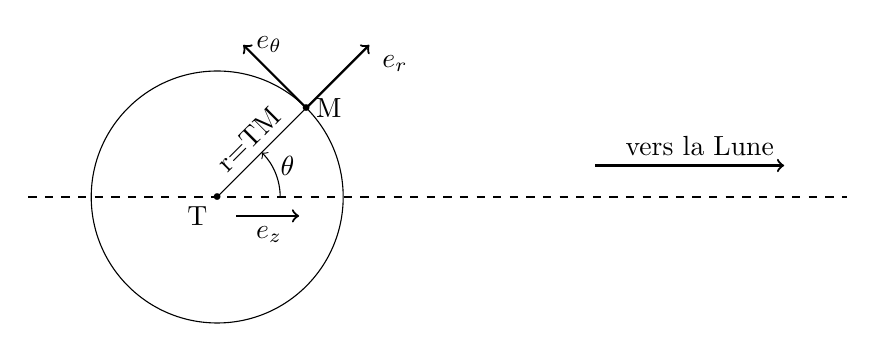
\begin{tikzpicture} [scale=0.8]
  \draw (0,0) circle(2) ;
  \draw [dashed] (-3,0) -- (10,0) ;
  \draw (0,0) -- (1.414,1.414) node [above,midway,sloped] {r=TM} ;
  \draw [-> , thick] (6,.5) --++ (3,0) node [above left] {vers la Lune} ;
  \draw (0,0) node {\tiny{$\bullet$}} node [below left] {T};
  \draw (1.414,1.414) node {\tiny{$\bullet$}} node [right] {M};
  \draw [-> , thick] (1.414,1.414) --++ (1,1) node [below right] {${\kern 1pt} \Vec {{e_r}}$} ;
  \draw [-> , thick] (1.414,1.414) --++ (-1,1) node [right] {${\kern 1pt} \Vec {{e_\theta}}$} ;
  \draw [-> , thick] (0.3,-0.3) --++ (1,0) node [below,midway] {${\kern 1pt} \Vec {{e_z}}$} ;
  \draw [->] (1,0)arc(0:45:1cm) ;
  \draw (0.85,0.5) node [right] {$\theta$} ;
  \end{tikzpicture}
  \capt{Développement limité du champ de marée en $r/d_L$.}
\end{fig}

  \begin{quest}
  \item Montrer que $\Vec {LM}  =  - {d_L}\Vec {{e_z}}  + r{\kern 1pt} \Vec {{e_r}} $.
  En déduire que, au premier ordre en $\frac{r}{{{d_L}}}$, on a
  \begin{equation}
    \frac{1}{{L{M^3}}} = \frac{1}{{d_L^3}}\left( {1 + \frac{{3r\cos (\theta )}}{{{d_L}}}} \right).
  \end{equation}

  \sol{
    On décompose les vecteur dans la base cylindrique d'axe TL. On a  
    $$
    \Vec{LM} = \Vec{LT} +  \Vec{TM} = -d_L \ez + r \er.
    $$
    Donc $LM^2 = d_L^2 + r^2 -2rd_L \ez \cdot \er = d_L^2 + r^2 - 2rd_L \cos(\theta) = d_L^2\left(1-2\frac{r}{d_L} \cos(\theta) + \left(\frac{r}{d_L}\right)^2 \right).$ On a donc
    \eqbox{
      LM^{-3} \simeq d_L^{-3}\left[1-2\frac{r}{d_L} \cos(\theta)  \right]^{-3/2} \simeq d_L^{-3}\left[1+3\frac{r}{d_L} \cos (\theta)\right].
    }
  }

  \item En déduire, toujours au premier ordre en $\frac{r}{{{d_L}}}$, que le champ de marée a pour expression simplifiée
  \begin{equation}
    \Vec {{C_L}} (M) =   \frac{{G{\kern 1pt} {m_L}}}{{{d_L}^3}}{\kern 1pt} r\left( {3\cos (\theta )\Vec {{e_z}}  - \Vec {{e_r}} } \right).
  \end{equation}

  \sol{
    On a $$
    \Vec {{C_L}} (M) = Gm_L\left(-\frac{\Vec{LM}}{LM^3} +\frac{\Vec{LT}}{LT^3} \right) \simeq \frac{Gm_L}{d_L^3}\left[-\left( 1+3\frac{r}{d_L} \cos (\theta)\right)(-d_L \ez + r \er) - d_L \ez \right] ,
    $$
    soit 
    \eqbox{
      \simeq \frac{Gm_L}{d_L^3}\left[ -3\frac{r}{d_L} \cos (\theta) (-d_L \ez) - r \er \right].
      }
  }

  \end{quest}

  En projetant $\Vec {{e_z}}$ sur la base $\left( {\Vec {{e_r}} ,\Vec {{e_\theta }} } \right)$, on obtient finalement
  \begin{equation}
    \Vec {{C_L}} (M) = \frac{{G{\kern 1pt} {m_L}r}}{{{d_L}^3}}{\kern 1pt} \left[ {\left( {3{{\cos }^2}(\theta ) - 1} \right)\Vec {{e_r}}  - 3\sin (\theta )\cos (\theta )\Vec {{e_\theta }} } \right].
  \end{equation}

  \begin{quest}
  \item Montrer que l'influence de la Lune sur les marées est de l'ordre de deux fois plus importante que celle du soleil.

  \sol{
  Le rapport du terme de marée Lunaire sur terme solaire est 
  \eqbox{
    \frac{C_L}{C_S}=\frac{m_L}{m_S}\left(\frac{d_S}{d_L}\right)^3 \simeq \num{2.2}.
    }
  }

  \item Préciser les positions relatives de la Terre, de la Lune et du Soleil pour les marées de vives eaux (amplitude maximale, les effets de la Lune et du Soleil s'ajoutent) et pour les marées de mortes eaux (amplitude minimale, les effets de la Lune et du Soleil se compensent partiellement). Attention à bien indiquer deux configurations distinctes pour chaque cas.
  Indiquer le lien avec les phases de la Lune et donner un ordre de grandeur de la périodicité de l'alternance vives-eaux/mortes-eaux.
  \sol{
  \begin{center}
  
\includegraphics[width=0.4\textwidth]{vive_morte.png}
  \end{center}
  Le cycle de vives-eaux / mortes-eaux vient de la superposition des effets de
  la lune et du soleil
  vives-eaux : nouvelle lune ou pleine lune
  mortes eaux : premier quartier et dernier quartier
  La période entre deux vives-eaux est d’une demi lunaison, soit 13,5 jours dans le modèle naïf où la Lune tourne autour d’une Terre fixe. Si on prend en compte le mouvement de la Terre autour du soleil , on trouve une lunaison de 29,5 jours, donc une période d’environ 15 jours.
  }
  \end{quest}


  % \bonus{
  \subsection{Amplitude des marées océaniques (bonus)}

  On considère dans cette partie un modèle simple : la Terre est entièrement recouverte d'eau. On obtient ainsi des résultats pertinents pour l'amplitude des marées en haute mer, mais qui n'expliquent pas les phénomènes observés près des côtes.
  On se place dans le cadre d'un modèle quasi-statique où la forme des océans à un instant donné obéit à la loi de l'hydrostatique ($p$ désigne la pression et $\Vec {{f_v}}$ la résultante des forces volumiques) :
  \begin{equation}
    \grad{p} = \Vec {{f_v}}.
  \end{equation}
  Dans toute cette partie on ne considère que l'influence de la Lune (et pas celle du Soleil). Le \emph{marnage}, que l'on notera $h$, est la différence de hauteur d'eau entre la marée haute et la marée basse en un endroit donné.

  \begin{quest}
  \item On commence par une approche dimensionnelle : on considère que, outre le facteur $\frac{{{m_L}}}{{{d_L}^3}}$ mis en évidence précédemment, la masse de la Terre $m_T$ et son rayon $R_T$ interviennent sur le marnage  et on pose :
  \begin{equation}
    h = \frac{{{m_L}}}{{{d_L}^3}}{m_T}^\alpha {R_T}^\beta.
  \end{equation}
    Déterminer les coefficients $\alpha$ et $\beta$ pour que $ h$ ait bien les dimensions d'une longueur et calculer numériquement la valeur de $ h$ qui en résulte.

  \sol{
  $[h] = M^{1+\alpha}L^{\beta-3} = L$ et donc $\alpha=-1$ et $\beta
  =4$. On trouve donc
  \eqbox{
    h \sim \frac{m_L R_T^4}{m_Td_L^3}  \simeq \SI{0.4}{m}.
  }
  }

  \item
  Que traduit la loi de l'hydrostatique ? Quelle est la dimension de ses termes ?
  Le terme $\Vec {{f_v}}$ traduit ici l'attraction gravitationnelle due à la Terre, celle due à la Lune ainsi que la force d'inertie d'entraînement dans le référentiel géocentrique $\RG$ due à la Lune. Donner l'expression de $\Vec {{f_v}}$ en utilisant, pour ce qui est des effets dus à la Lune, l'expression de $\Vec{C_L}(M)$ donnée dans la \Sec{champ}. On notera $\mu$ la masse volumique de l'eau.

  \sol{
  La loi de l’hydrostatique traduit l’équilibre du fluide (PFD appliqué à une particule de fluide immobile). La force volumique a pour dimension $[f_v] = M L^{-2} T^{-2}$.
  La force volumique de marée vaut
  \eqbox{
    \Vec{f_v} = \mu \Vec{C_L}(M) + \mu \Vec{\mc{G}_T}(M) = \frac{{\mu G{\kern 1pt} {m_L}r}}{{{d_L}^3}}{\kern 1pt} \left[ {\left( {3{{\cos }^2}(\theta ) - 1} \right)\Vec {{e_r}}  - 3\sin (\theta )\cos (\theta )\Vec {{e_\theta }} } \right] - \frac{\mu G m_T}{R_T^2} \er.
    }
  }
  \end{quest}
   On pose $\Vec {{f_v}}  =- \grad ({V_T} + {V_L})$, où $V_T$ est l'énergie potentielle volumique associée à l'attraction gravitationnelle de la Terre et $V_L$ l'énergie potentielle volumique associée aux effets dus à la Lune.
  On donne l'expression du gradient d'une fonction scalaire $f$ en coordonnées sphériques : 
  \begin{equation}
    \grad{f} = \frac{{\partial f}}{{\partial r}}\Vec {{e_r}}  + \frac{1}{r}\frac{{\partial f}}{{\partial \theta }}\Vec {{e_\theta }}  + \frac{1}{{r\sin (\theta )}}\frac{{\partial f}}{{\partial \varphi }}\Vec {{e_\varphi }}.
  \end{equation}
  \begin{quest}

  \item
  Établir l'expression de $V_T(r)$, en proposant un choix naturel pour la constante d'intégration. Montrer ensuite que la fonction
  \begin{equation}
    V_L(r,\theta) = -\frac{\mu G m_L}{2 d_L^{3}} r^2(3\cos^2(\theta)-1)
  \end{equation}
  conduit bien à l'expression de $\Vec{f_v}$.

  \sol{
  L’énergie potentielle volumique $V_T$ liée à l’attraction terrestre est telle que
  $$
  \mu \Vec{\mc{G}_T}(M) = - \frac{\mu G m_T}{r^2} \er = -\grad V_T = - \dr{V_T}{r} \er.
  $$
  donc $V_T(r) = - \frac{\mu G m_T}{r} + \cte $, soit 
  \eqbox{
    V_T(r)  = - \frac{\mu G m_T}{r} 
  } en prenant $V_T(r=\infty) = 0$. On vérifie ensuite que l'expression de $V_L$ convient.
  \begin{align*}
  -\grad{V_L} & = -\frac{{\partial V_L}}{{\partial r}}\Vec {{e_r}}  - \frac{1}{r}\frac{{\partial V_L}}{{\partial \theta }}\Vec {{e_\theta }} \\
  & = \frac{\mu G m_L}{2 d_L^3}\left[ \dr{r^2}{r}(3\cos^2\theta-1) \er + \frac{r^2}{r} \dr{}{\theta}(3\cos^2\theta-1)\,\et \right] \\
  & = \frac{\mu G m_L}{2 d_L^3}\left[2r(3\cos^2\theta-1) \er + 6\cos \theta\, \sin \theta \,\et \right] \\
  & = \frac{{\mu G{\kern 1pt} {m_L}r}}{{{d_L}^3}}{\kern 1pt} \left( {\left( {3{{\cos }^2}(\theta ) - 1} \right)\Vec {{e_r}}  - 3\sin (\theta )\cos (\theta )\Vec {{e_\theta }} } \right)  \\
  &  = \mu \Vec{C_L}(M).
  \end{align*}
On a bien $-\Grad{V_L + V_T} = \mu \Vec{C_L}(M) + \mu \Vec{\mc{G}_T}(M) = \Vec{f_v}  $.
  }

  \item
  La pression atmosphérique est considérée comme uniforme à la surface de l'eau. Montrer que dans ces conditions la surface de l'eau vérifie $V_T + V_L = \cte$. En déduire que, toujours à la surface de l'eau,
  \begin{equation}
    \frac{{{m_T}}}{r} + \frac{{{m_L}}}{{{d_L}^3}}\frac{{{r^2}}}{2}\left( {3{{\cos }^2}(\theta ) - 1} \right) = A = \text{constante}.
  \end{equation}

  \sol{
  La loi de l’hydrostatique dans le référentiel géocentrique $\RG$ s’écrit
  $$\grad{p} = \Vec{f_v} = - \grad (V_T+V_L), $$
   et donc $\grad (V_T+V_L+p) = \Vec{0}$ et $V_T+V_L+p = \cte$. La surface de l'eau est une isobare  à la pression atmosphérique $p_0$, et donc $p=p_0=\cte$. On a donc également
  \eqbox{V_T+V_L=\cte = -\mu G A.}
  En divisant par $-\mu G$, on trouve bien la relation attendue 
  \eqbox{
    \frac{{{m_T}}}{r} + \frac{{{m_L}}}{{{d_L}^3}}\frac{{{r^2}}}{2}\left( {3{{\cos }^2}(\theta ) - 1} \right) = A .
  }
  }

  \item On détermine (en écrivant que, l'eau étant considérée comme incompressible, le volume des océans est le même avec et sans déformation) que la constante introduite précédemment vaut $A=\frac{{{m_T}}}{{{R_T}}}$.  Le marnage $h$ étant petit par rapport à $R_T$, on pose $r=R_T+h$ avec $\frac{h}{{{R_T}}} \ll 1$. En effectuant les développements limités adéquats au premier ordre en $\frac{h}{{{R_T}}}$ , montrer que : 
  \begin{equation}
    A \simeq 
    % \left[ 
      {\frac{{{m_T}}}{{{R_T}^2}} - \frac{{{m_L}{\kern 1pt} {R_T}}}{{{d_L}^3}}\left( {3{{\cos }^2}(\theta ) - 1} \right)}.
      %  \right]. 
    % \simeq
    %  \frac{{{m_L}{\kern 1pt} {R_T}^2}}{{2{d_L}^3}}\left( {3{{\cos }^2}(\theta ) - 1} \right).
  \end{equation}
  Vérifier numériquement que $\frac{{{m_L}{\kern 1pt} {R_T}}}{{{d_L}^3}} \ll \frac{{{m_T}}}{{{R_T}^2}}$, et en déduire l'expression de $h$ simplifiée  en conséquence. On utilisera cette expression simplifiée dans les deux questions suivantes.


  \sol{
  On a $r^{-1} \simeq R_T^{-1}(1-\frac{h}{R_T})$ et $r^{2} \simeq R_T^{2}(1+2\frac{h}{R_T})$. Puis
  \eqbox{h = \frac{m_L R_T^4}{2 m_T d_L^3}(3\cos^2(\theta)-1).}
  On évalue le rapport 
  \eqbox{
  \frac{m_LR_T^4}{2m_Td_L^3} \sim \SI{0.19}{m}.
  }
  }

  \item Pour simplifier, on considère que la Lune reste dans le plan équatorial de la Terre. Où le marnage $h$ est-il le plus important ? Que peut-on dire du marnage aux pôles ?

  \sol{
  Le marnage est maximal, comme attendu, pour $\theta=0$ et $\theta=\pi$ (à l'équateur). Il est négatif et d'amplitude moitié aux pôles pour $\theta=\frac{\pi}{2}$.
  }

  \item Établir l'expression du marnage $h_E$ à l'équateur et faire l'application numérique. Comparer au marnage à Saint-Malo donné sur la \Fig{manche}. Que peut-on dire de l'effet des côtes.

  \sol{
    À l'équateur on trouve exactement la valeur issue de l'analyse dimensionnelle,
    \eqbox{
    h_E = \frac{m_L R_T^4}{m_T d_L^3} = \SI{0.4}{m}.
    }
    On voit que la valeur de $h$ prédite est bien plus petit que celle mesurée ! Il faut prendre en compte l'effet des côtes.
  }
  % }

  \end{quest}
\end{exo}
%%%%%%%%%%%%%%%%%%%%%%%%%%%%%%%%%%%

%%%%%%%%%%%%%%%%%%%%%%%%%%%%%%%%%%%
\begin{exo}[PC][1][devoir]{Modélisation du mouvement d'une plateforme en mer}
  \Annale[Modélisation PC]{CCINP}{2019}
  On s'intéresse à la résolution d'équations du mouvement dans une approche classique de la mécanique afin d'étudier le mouvement d'une plateforme en mer. Le modèle envisagé est un système à un degré de liberté considéré comme oscillateur harmonique : une masse est reliée à un ressort, avec ou sans amortissement, et peut être soumise à une excitation externe.

  \begin{fig}[]
    \centering
    \begin{subfig}[label][0.45]
      
\includegraphics[width=\textwidth]{2023_08_30_f71d0d57c198e5ec6d06g-02(1)}
    \end{subfig}
    \begin{subfig}[label][0.45]
      
\includegraphics[width=\textwidth]{2023_08_30_f71d0d57c198e5ec6d06g-02}
    \end{subfig}
    \capt{(a) Plateforme en mer soumise aux vagues marines, (b) système masse $(m)$, ressort $(k)$, amortisseur $(\gamma)$ et excitation externe $(\F_{\text{exc}})$}
  \end{fig}

  % La résolution est tout d'abord abordée de façon analytique puis de façon numérique, avant enfin de comparer les résultats obtenus.

  % Les résolutions analytiques et numériques sont largement indépendantes.
  %
  % Dans la suite de l'énoncé, toutes les grandeurs vectorielles sont indiquées en gras.
  %
  % Un aide-mémoire sur numpy est donné en Annexe.

  On considère le mouvement d'une plateforme en mer soumise à un courant marin. Sa partie supérieure de masse $m=110$ tonnes est considérée comme rigide et le mouvement principal de la plateforme a lieu suivant $x$ (figure 1(a)).

  Afin d'étudier le mouvement de cette plateforme, on la représente par une masse $m$, liée à un ressort de constante de raideur $k$ et à un amortisseur de constante d'amortissement $\gamma$, pouvant subir une excitation externe de force $\F_{\text{exc}}$, et se déplaçant sur un support (figure 1(b)). Le ressort représente la rigidité de l'ensemble du support de la plateforme. L'amortisseur permet de prendre en compte l'effet de l'eau environnante et la force d'excitation externe celui des vagues qui frappent périodiquement la plateforme. La masse est supposée se déplacer selon une seule direction parallèle à l'axe $(Ox)$ en fonction du temps $t$.



  Les projections sur l'axe $(Ox)$ de la position, de la vitesse et de l'accélération de la masse en fonction du temps sont notées respectivement $x(t), \dot{x}(t)$ et $\ddot{x}(t)$. La force totale $\F_{\text {tot }}$ agissant sur la masse correspond à la réaction normale $\Vec{R}_{N}$ de la base horizontale, à la force de frottement $\F_{d}$, à la force de rappel $\F_{k}$ du ressort, au poids $\Vec{P}$ de la masse et à la force $\F_{\text {exc }}$ d'excitation externe. La position d'équilibre de la masse sera choisie à $x=0$. En l'absence d'action de l'amortisseur, la masse se déplace sur la base horizontale sans frottements.

  % \subsection{Résolution analytique et détermination des paramètres pour la modélisation
   % dynamique du point sans changement de référentiels}
   \begin{quest}
  \item En effectuant une projection sur l'axe $(Ox)$, montrer que $\Vec{P}$ et $\Vec{R}_{N}$ n'interviennent pas dans le bilan des forces.

  \sol{
  On applique le PFD dans le référentiel terrestre, galiléen. Le bilan des forces est donné par l'énoncé, on obtient:
  $$
   m\vv{a}=\sum \vv{F}=\vv{R_N}+\vv{F_d}+\vv{F_k}+\vv{P}+\vv{F_{exc}}
  $$
  Le mouvement est suivant $\ex$ uniquement, la projection sur la verticale  $(Oz)$  indique que le poids et $\vv{R_N}$ s'annulent, et suivant l'horizontale on obtient l'équation du mouvement:
  $$
   \boxed{m\ddot{x}=0+F_d+F_k+0+F_{\rm exc}}
  $$
  Le poids et la réaction normale n'interviennent pas dans cette équation du mouvement, mais font cependant bel et bien partie du bilan des forces.
  }
\end{quest}



  \subsection{Ressort sans amortissement et sans excitation}
\begin{quest}
  \item Démontrer que l'équation du mouvement de la masse correspond à l'équation différentielle du second ordre suivante :

  % $$
  \begin{equation}
    m \ddot{x}+k x=0 .
  \end{equation}
  % $$

  \sol{
   $F_d=0=F_{exc}$ traduit les conditions de travail de cette partie, et la force élastique est une force de rappel vers la position d'équilibre. Dans la limite d'élasticité de la structure, $F_k=-k x$ puisque la position d'équilibre est choisie comme origine de l'axe horizontal. On a donc bien finalement $$\boxed{ m\ddot{x} + kx = 0}.$$
  }

  \item La solution de cette équation prend la forme générale suivante

  % $$
  \begin{equation}
    x(t)=A_{0} \sin \left(\omega_{0} t\right)+B_{0} \cos \left(\omega_{0} t\right)
  \end{equation}
  % $$

  avec $A_{0}$ et $B_{0}$ deux coefficients réels. Exprimer $\omega_{0}$ en fonction des grandeurs caractéristiques du système et donner sa signification physique. De plus, en remarquant qu'à $t=0: x(t)=x_{0}$ et $\dot{x}(t)=\dot{x}_{0}$, déterminer les expressions de $A_{0}$ et de $B_{0}$ en fonction de $x_{0}, \dot{x}_{0}$ et de $\omega_{0}$.

  \sol{
  L'équation différentielle obtenue est celle d'un oscillateur harmonique de \underline{pulsation propre} $\boxed{\omega_0=\sqrt{\frac{k}{m}}}$, cette pulsation est celle des \underline{oscillations libres} de ce système.
  La condition initiale sur la position donne $x(t=0)=\boxed{x_0=B_0}$ et celle sur la vitesse $\omega_0 A_0=\dot{x}_0$, soit $\boxed{A_0=\frac{\dot{x}_0}{\omega_0}}$ et donc $$\boxed{x(t)=x_0\cos{\omega_0 t}+\frac{\dot{x}_0}{\omega_0}\sin{\omega_0 t}}.$$
  }

  \item On cherche à reformuler l'équation précédente sous une forme plus compacte du type :

  % $$
  \begin{equation}
    x(t)=R_{0} \cos \left(\omega_{0} t-\phi_{0}\right) .
  \end{equation}
  % $$

  Donner les expressions de $R_{0}$ et de $\phi_{0}$ en fonction de $x_{0}, \dot{x}_{0}$ et de $\omega_{0}$.
  \sol{
  $$
   x(t) = R_0 \cos(\omega_0t - \phi_0)=R_0(\cos(\omega_0t)\cos(\phi_0)+\sin(\omega_0t)\sin(\phi_0)
$$
  Par identification avec $x(t) = A_0 \sin(\omega_0t) + B_0 \cos(\omega_0t)$, il vient:
  $$
   \begin{cases}
    A_0=R_0\sin(\phi_0)\\
    B_0=R_0\cos(\phi_0)
   \end{cases}
  $$
  Ce qui permet d'obtenir $R_0$ et $\phi_0$ en réinjectant les résultats de la question précédente:

  $$
  \begin{cases}
    R_0=\sqrt{A_0^2+B_0^2}=\sqrt{x_0^2+\left(\frac{\dot x_0}{\omega_0}\right)^2}\\
    \tan(\phi_0)=\frac{A_0}{B_0}=\frac{\dot x_0}{\omega_0 x_0}\\
   \end{cases}
   $$
  }

  \item Représenter qualitativement $x(t)$ en fonction de $t$ et indiquer sur le tracé $R_{0}, x_{0}$ et $2 \pi / \omega_{0}$.
  \sol{
  $R_0$ est l'amplitude de la sinusoïde, $x_0$ sa valeur à $t=0$ et $2\pi/\omega_0$ la période:
\begin{center}
  
  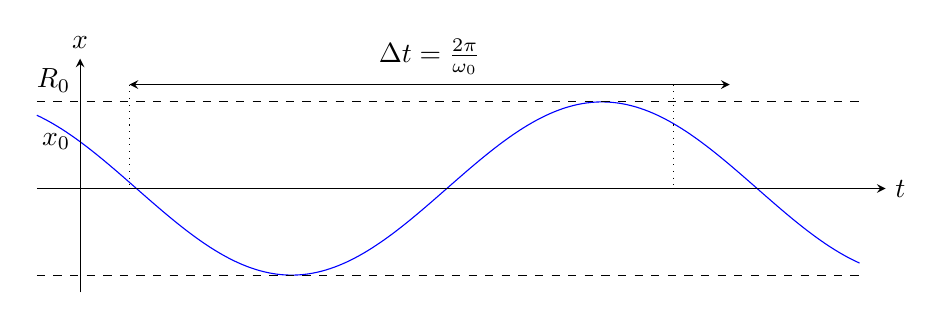
\begin{tikzpicture}[>=stealth,scale=1.1]
    \draw [blue] plot[samples=100,domain=-0.5:9, samples=200] (\x,{cos(16*3.14*\x + 1 r)});
    \draw [->] (-0.5,0) -- (9.3,0) node[right] {$t$};
    \draw [thin, dashed] (-0.5,1) -- (9,1);
    \draw [thin, dashed] (-0.5,-1) -- (9,-1);
    \draw [->] (0,-1.2) -- (0,1.5) node[above] {$x$};
    \draw (0,0.54) node [left] {$x_0$} (0,1) node[above left]{$R_0$};
    \draw[<->] (0.57,1.2) -- (7.5,1.2) node[pos=0.5,above] {$\Delta t=\frac{2\pi}{\omega_0}$};
    \draw[thin, dotted] (0.57,1.2) -- (0.57,0) (6.85,1.2) --(6.85,0) ;
  \end{tikzpicture}
\end{center}

  }

  \item En utilisant les expressions des énergies cinétique $K(t)$ et potentielle $U(t)$ du système, montrer que l'énergie totale $E(t)$ du système est alors :

  % $$
  \begin{equation}
    E(t)=\frac{k R_{0}^{2}}{2}
  \end{equation}
  % $$

  Justifier le résultat obtenu.
  \sol{

  \begin{liste}
    \item   Par définition de l'énergie cinétique, $K(t)=\frac{1}{2}mv^2= \frac{1}{2}m\left(-R_0\omega_0\sin(\omega_0t-\phi_0)\right)^2=\frac{1}{2}mR^2_0\omega_0^2\sin^2(\omega_0t-\phi_0)$.
    \item   Pour un système élastique de constante de raideur $k$, l'énergie potentielle élastique s'exprime sous la forme $U=\frac{1}{2}kx^2$, soit $U(t)=\frac{1}{2}k^2R^2_0 \cos^2(\omega_0t - \phi_0)$.
  \end{liste}

Avec $\omega_0^2=k/m$, on en déduit $E(t)=K(t)+U(t)=\frac{1}{2}kR^2_0\sin^2(\omega_0t-\phi_0)+\frac{1}{2}k^2R^2_0 \cos^2(\omega_0t - \phi_0)$, soit $$\boxed{\frac{1}{2}kR^2_0.}$$

  $E$ est une constante car il n'y a que des forces conservatives. Lorsque l'énergie cinétique est nulle, le déplacement esst maximal, vaut $\pm R_0$ et toute l'énergie est sous forme potentielle élastique, d'où cette expression de cette constante.
  }

  \item Représenter qualitativement $E(t), K(t)$ et $U(t)$ en fonction de $t$.
  \sol{
\begin{center}
  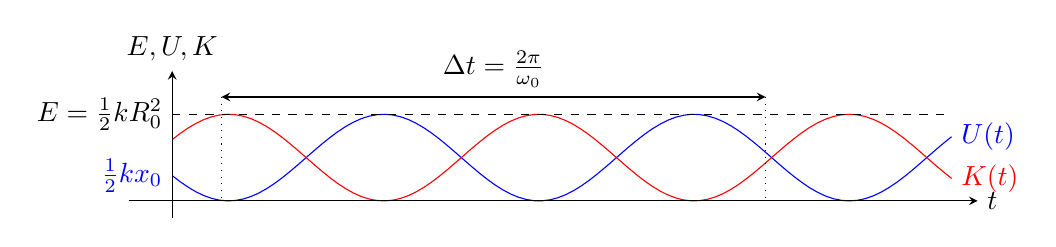
\begin{tikzpicture}[>=stealth,scale=1.1]
    \draw [blue] plot[samples=100,domain=-0.0:9] (\x,{cos(16*3.14*\x + 1 r)^2}) node[right] {$U(t)$} (0,0.29) node [left] {$\frac{1}{2}k x_0$};
    \draw [red] plot[samples=100,domain=-0.0:9] (\x,{sin(16*3.14*\x + 1 r)^2}) node[right] {$K(t)$};
    \draw [->] (-0.5,0) -- (9.3,0) node[right] {$t$};
    \draw [->] (0,-.2) -- (0,1.5) node[above] {$E,U,K$};
    \draw [thin, dashed] (-0.,1) -- (9,1);
    \draw  (0.,1) node[left]{$E=\frac{1}{2}kR^2_0$};
    \draw[<->] (0.57,1.2) -- (6.85,1.2) node[pos=0.5,above] {$\Delta t=\frac{2\pi}{\omega_0}$};
    \draw[thin, dotted] (0.57,1.2) -- (0.57,0) (6.85,1.2) --(6.85,0) ;
  \end{tikzpicture}
\end{center}

  }
\end{quest}


  \subsection{Ressort avec amortissement et sans excitation}
  \begin{quest}
  \item La force de frottement que l'amortisseur exerce sur la masse est considérée comme linéaire, c'est-à-dire proportionnelle au vecteur vitesse $\Vec{v}$ de celle-ci : $\F_{d}=-\gamma \Vec{v}$, avec $\gamma$ constante d'amortissement $(>0)$. En considérant une projection sur l'axe $(Ox)$, démontrer que la position de la masse en fonction du temps suit l'équation du mouvement ci-après

  % $$
  % \begin{equation}
  \begin{equation}
    \ddot{x}+2 \zeta \omega_{0} \dot{x}+\omega_{0}^{2} x= 0
  \end{equation}
  % \end{equation}
  % $$

  avec $\omega_{0}$ défini en question 3 et $\zeta$ à exprimer en fonction de $\gamma, k$ et $m$.

  \sol{
   On repart de la question~\ref{ques:2019-CCPINP-Q1-ques} avec $F_d=-\gamma \dot{x}$ et toujours $F_{exc}=0$, on obtient $\boxed{\ddot{x}+\frac{\gamma}{m}+\frac{k}{m}x=0}$. Par identification avec la forme de l'équation~\ref{eq:2019-CCPINP-EQ5}, on obtient bien $\omega_0^2=k/m$ comme précédemment, et $2\xi\omega_0=\frac{\gamma}{m}$, ce qui donne $\boxed{\xi=\frac{\gamma}{2\sqrt{mk}}}$
  }

  \item Dans le cas où $\zeta<1$, la fonction $x(t)$ prend la forme suivante :

  % $$
  \begin{equation}
    x(t)=e^{-\zeta \omega_{0} t}\left(A_{\mathrm{d}} \cos \left(\omega_{\mathrm{d}} t\right)+B_{\mathrm{d}} \sin \left(\omega_{\mathrm{d}} t\right)\right) .
  \end{equation}
  % $$

  Déterminer les deux coefficients réels $A_{\mathrm{d}}$ et $B_{\mathrm{d}}$ en fonction de $x_{0}, \dot{x}_{0}, \zeta, \omega_{0}$ et $\omega_{\mathrm{d}}=\omega_{0}  \sqrt{1-\zeta^{2}}$. On utilisera pour cela les mêmes conditions initiales que celles utilisées en question 3.

  \sol{
  À $t=0$, $x(t=0)=x_0=A_d e^0$, donc $\boxed{A_d=x_0}$. On calcule ensuite $\dot x$ pour pouvoir utiliser la seconde condition initiale:
  $$
   \dot x(t)=e^{-\xi \omega_0 t}\left((-\xi \omega_0x_0 +B_d \omega_d)\cos( \omega_d t)+(-\xi \omega_0 B_d-x_0 \omega_d)\sin( \omega_d t)\right)
  $$
 d'où $\dot x(t=0)=-\xi \omega_0x_0 +B_d \omega_d=\dot x_0$ et donc $\boxed{B_d=\frac{\dot x_0+\xi \omega_0x_0}{ \omega_d}}$
  }



  \item Montrer alors que l'on peut obtenir une forme du type

  % $$
  \begin{equation}
    x(t)=R_{\mathrm{d}} e^{-\zeta \omega_{0} t} \cos \left(\omega_{\mathrm{d}} t-\phi_{\mathrm{d}}\right)
  \end{equation}
  % $$

  avec $R_{\mathrm{d}}$ et $\phi_{\mathrm{d}}$ à préciser.

  \sol{

  On développe $\cos(\omega_dt - \phi_d)=\cos(\omega_dt)\cos(\phi_d)+\sin(\omega_dt)\sin(\phi_d)$, ce qui permet d'identifier les termes entre les deux formes
  $\begin{cases}
    A_d=R_d\cos(\phi_d)\\
    B_d=R_d\sin(\phi_d)
   \end{cases}$ ce qui donne
   \eqbox{
     \begin{cases}
      R_d=\sqrt{A_d^2+B_d^2}\\
      \tan(\phi_d)=B_d/A_d
    \end{cases}
    }
  On pourrait réinjecter les valeurs de $A_d$ et $B_d$ en fonction des conditions initiales, mais ce n'est pas explicitement demandé et sans intérêt majeur.
  }

  \item Représenter qualitativement $x(t)$ en fonction de $t$ et indiquer sur le tracé $R_{\mathrm{d}} e^{-\zeta \omega_{0} t}, x_{0}$ et $2 \pi / \omega_{\mathrm{d}}$.

  \sol{
    \begin{center}
      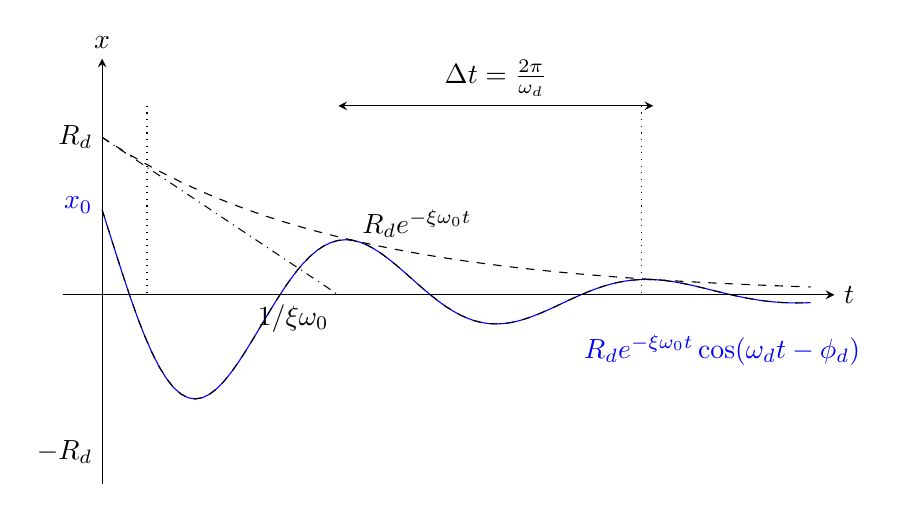
\begin{tikzpicture}[>=stealth,yscale=2]
        \draw [blue] plot[samples=100,domain=-0.0:9] (\x,{exp(-\x/3)*cos(30*3.14*\x + 1 r)}) ++(-3,-0.3) node[right]  {$R_de^{-\xi\omega_0 t}\cos(\omega_dt - \phi_d)$} (0,0.57) node [left] {$x_0$};
  \draw [dashed] plot[samples=100,domain=-0.0:9] (\x,{exp(-\x/3)*cos(30*3.14*\x + 1 r)}) ++(-5,0.5) node {$R_de^{-\xi\omega_0 t}$} (0,1) node [left] {$R_d$};
  \draw [->] (-0.5,0) -- (9.3,0) node[right] {$t$};
  \draw [->] (0,-1.2) -- (0,1.5) node[above] {$x$};
  \draw [dashed] plot[samples=100,domain=-0.0:9] (\x,{exp(-\x/3)}) (0,-1) node [left] {$-R_d$};
  \draw[<->] (3,1.2) -- (7,1.2) node[pos=0.5,above] {$\Delta t=\frac{2\pi}{\omega_d}$};
  \draw[thin, dotted] (0.57,1.2) -- (0.57,0) (6.85,1.2) --(6.85,0) ;
  \draw[thin,dashdotted] (0,1) -- (3,0) node [below left] {$1/\xi\omega_0$};
\end{tikzpicture}
\end{center}
  }

  \item Donner l'expression de $E(t)$ et commenter les cas où $\zeta=0$ et $\zeta=1$.
  \sol{
  Pour $\xi = 0$, l'énergie $E$ est constante: c'est le cas étudié précédemment.
  Pour $\xi = 1$, $\omega_d=0$ les expressions obtenues précédemment ne sont plus valables car cela correspond au régime critique et donc plus au régime pseudo-périodique sur lequel les expressions fournies par l'énoncé sont valables. On a alors un retour à l'équilibre particulièrement rapide.
  Pour $1> \xi > 0$, on peut essayer de se laisser guider par le calcul précédent:
  $$
   \begin{array}{rl}
    E(t)&=K(t)+U(t)=\frac{1}{2}m\dot x^2+\frac{1}{2}k x^2=\frac{1}{2}k\frac {\dot x^2}{\omega_0^2}+\frac{1}{2}k x^2\\
    &=\frac{1}{2}k R_d^2\left(\frac{\mathrm d\,\left( 
      e^{-\xi\omega_0 t} \cos(\omega_dt - \phi_d)\right)}{\omega_0\mathrm d\,t}\right)^2+\frac{1}{2}k^2 R_d^2 e^{-2\xi\omega_0 t} \cos^2(\omega_dt - \phi_d)\\
    &=\frac{1}{2}k R_d^2\left[
      e^{-2\xi\omega_0 t}\left(-\xi\cos(\omega_dt - \phi_d)-\frac{\omega_d}{\omega_0}\sin(\omega_dt - \phi_d)\right)^2+e^{-2\xi\omega_0 t} \cos^2(\omega_dt - \phi_d)\right]\\
    &=\frac{1}{2}k R_d^2 e^{-2\xi\omega_0 t} \left(\xi^2\cos^2(\omega_dt - \phi_d)+(1-\xi^2)\sin^2(\omega_dt - \phi_d)+\ldots
    \right.\\
    &\quad\quad\quad\ldots\left.+2\xi\sqrt{1-\xi^2}\cos(\omega_dt - \phi_d)\sin(\omega_dt - \phi_d)+\cos^2(\omega_dt - \phi_d)
    \right)\\
    &=\frac{1}{2}k R_d^2 e^{-2\xi\omega_0 t} \left(1+\xi^2\left(\cos^2(\omega_dt - \phi_d)-\sin^2(\omega_dt - \phi_d)\right)+2\xi\sqrt{1-\xi^2}\cos(\omega_dt - \phi_d)\sin(\omega_dt - \phi_d)\right)\\
   \end{array}
  $$
  donc
  \eqbox{
  \frac{1}{2}k R_d^2 e^{-2\xi\omega_0 t} \left(1+\xi^2\cos(2\omega_dt - 2\phi_d)+\xi\sqrt{1-\xi^2}\sin(2\omega_dt - 2\phi_d)\right).
  }
  On retrouve bien la valeur constante pour $\xi = 0$. Pour $\xi \rightarrow 1$ dans cette expression, le régime devient critique puisque $\omega_d=0$. On a alors une décroissance exponentielle de l'énergie selon $E(t)=E_0e^{-2\omega_0 t}$.
  }

  \item Montrer de façon simple que $E$ est une fonction décroissante de $t$. À quoi cela est-il dû?

  \sol{
  Le théorème de l'énergie mécanique écrit sur les puissances nous indique que la dérivée temporelle de $E$ est égale à la puissance des forces non conservatives, c'est-à-dire ici la puissance de la force de frottement:
  \eqbox{
   \frac{\mathrm d\,E}{\mathrm d\,t}=-\gamma\vv{v}\cdot\vv{v}=-\gamma\dot{x}^2
  }
  $\gamma$ étant une constante positive, cette expression est nécessairement toujours négative et l'énergie totale $E$ est bien une fonction décroissante du temps.
  C'est dû à la caractéristique principale de toute force de frottement, qui s'oppose toujours a déplacement (ce qui ce traduit dans les équations en imposant $\gamma>0$).
  }

  \item On envisage deux temps successifs $t_{1}$ et $t_{2}$ pour lesquels les déplacements sont $x_{1}$ et $x_{2}$, tels que $t_{2}>t_{1}$ et $t_{2}-t_{1}=\tau_{\mathrm{d}}$, avec $\tau_{\mathrm{d}}$ : période des oscillations amorties. En utilisant l'équation (7) et en considérant que $\zeta \ll 1$, montrer que :

  % $$
  \begin{equation}
    \ln \left(x_{1} / x_{2}\right) \approx  2 \pi \zeta .
  \end{equation}
  % $$

  \sol{
  Les deux instants étant séparés d'une période de la fonction sinusoïdale, les cosinus ont la même valeur et se simplifient en faisant le rapport, tout comme l'amplitude $R_d$. Dès lors il ne reste dans ce rapport que les termes exponentiels:
  $$
   \ln(x_1/x_2)=\ln\left(\frac{e^{-\xi\omega_0 t_1}}{e^{-\xi\omega_0 t_2}}\right)=\xi\omega_0(t_2-t_1)=\xi\omega_0\frac{2\pi}{\omega_d}=\frac{2\pi\xi}{\sqrt{1-\xi^2}}
  $$
  Dans la limite $\xi \ll 1$, $\sqrt{1-\xi^2}\approx 1$ et on obtient bien $\boxed{\ln(x_1/x_2) \approx 2\pi \xi}$
  }

  \item Le relevé du déplacement horizontal de la plateforme en fonction du temps est représenté en figure 2.

  En utilisant les deux points qui sont indiqués sur la figure, déterminer $k, \zeta$ et $\gamma$. Comment ce tracé serait modifié en fonction de la valeur de $\zeta$ ?
\end{quest}

\begin{fig}[]
  \centering
  
\includegraphics[width=0.45\textwidth]{2023_08_30_f71d0d57c198e5ec6d06g-04}
  \capt{ Relevé du déplacement horizontal $x$ (en $\mathrm{m}$) de la plateforme de masse $m=110$ tonnes en fonction du temps $t$ (en s). Les deux temps $t_{1}$ et $t_{2}$ mentionnés en question  sont indiqués.}
\end{fig}

\sol{
La figure nous indique 2 points séparés d'une période de la pseudo-oscillation, on utilise pour ces points le résultat précédent. Avec $x_1=\SI{1.4602}{cm}$ et $x_2=\SI{1.0661}{cm}$, $\xi=\frac{1}{2\pi}\ln(x_1/x_2)=\boxed{\num{5.01e-2}=\xi}$. La condition $\xi \ll 1$ est raisonnablement vérifiée.
En conservant la même approximation, on a $\omega_d\approx \omega_0$, qui peut être évalué via les valeurs de $t_1$ et $t_2$: $\omega_0\approx\frac{2\pi}{t_2-t_1}$. Comme $k=m\omega^2_0$, $\boxed{k=m\left(\frac{2\pi}{t_2-t_1}\right)^2=\SI{2.71e5}{kg.s^{-2}}}$.
Enfin, $\boxed{\gamma=2\xi\sqrt{mk}=\SI{1.73e4}{kg.s^{-1}}}$.

Lorsque le coefficient d'amortissement $\xi$ augmente, la décroissance est plus rapide, et lorsqu'on quitte la condition $\xi \ll 1$, la période des pseudo-oscillation augmente ($\omega_d$ décroit avec la croissance  de $\xi$)
}

  \subsection{Ressort avec amortissement et avec excitation}
  On envisage enfin le cas où le système est soumis à la fois aux effets d'amortissement et d'excitation. On se limite ici à la réponse à une excitation harmonique sinusoïdale de fréquence $\omega$ produite par une force extérieure au système

  % $$
  \begin{equation}
    \F_{\text{exc}}(t)=F_{0} \cos (\omega t) \ex
  \end{equation}
  % $$

  avec $\Vec{e}_{\Vec{x}}$ vecteur unitaire sur l'axe $(Ox)$ et on se place dans le cas traité précédemment pour l'étude de l'amortisseur, c'est-à-dire $\zeta<1$ (I.2).

  On admet de plus dans ce qui suit que la réponse du système dans le cas où amortisseur et excitation sont pris en compte peut s'écrire comme somme de la solution donnée par l'équation (6) et de la contribution due à l'excitation :

  % $$
  \begin{equation}
    x_{\mathrm{exc}}(t)=X \cos (\omega t-\phi)
  \end{equation}
  % $$

  \begin{quest}

  \item Montrer que l'équation différentielle caractérisant le système devient alors :

  % $$
  \begin{equation}
    \ddot{x}+2 \zeta \omega_{0} \dot{x}+\omega_{0}^{2} x=\frac{F_{0}}{m} \cos (\omega t).
  \end{equation}
  % $$

  \sol{
  On reprend le PFD établit à la question~\ref{ques:2019-CCPINP-Q1-ques}, et on obtient pour la projection de ce PFD sur l'axe $Ox$ $m\ddot x=-\gamma\dot{x}-kx+F_0 \cos(\omega t)$, ce qui se réécrit:
  $$
   \boxed{\ddot x+\frac{\gamma}{m}\dot{x}+\frac{k}{m}x=\frac{F_0}{m} \cos(\omega t)}
  $$
  On a bien l'expression voulue en gardant comme précédemment $\omega^2_0=\frac{k}{m}$ et $2\xi\omega_0=\frac{\gamma}{m}$

  }

  \item En utilisant l'équation (10) et en privilégiant une représentation complexe, vérifier que :

  $$
  \left\{\begin{array}{l}
  X=\frac{F_{0}}{m} \cdot \frac{1}{\sqrt{\left(\omega_{0}^{2}-\omega^{2}\right)^{2}+\left(2 \zeta \omega_{0} \omega\right)^{2}}} \\
  \tan \phi=\frac{2 \zeta \omega_{0} \omega}{\omega_{0}^{2}-\omega^{2}}
  \end{array} .\right.
  $$

  \sol{
  L'équation différentielle étant linéaire, traiter la solution particulière et la solution de l'équation homogène séparément pour ensuite les additionner et obtenir l'ensemble des solutions ne surprend guère.

  On introduit les représentations complexes des grandeurs évoluant sinusoïdalement, la grandeur complexe est soulignée:
  $$
  X(t)=X_0 \cos(\omega t+\phi)\leftrightarrow \underline{X}(t)=X_0 e^{j\omega t+\phi}=\underline{X_0}e^{j\omega t}
  $$

  Pour les représentations complexes des grandeurs, l'équation~\ref{eq:2019-CCPINP-EQ11} devient, les exponentielles se factorisant puis pouvant être simplifiées (une dérivée temporelle devient une multiplication par $j\omega$):

  $$
  \underline{X}\left(-\omega^2+2\xi\omega_0j\omega+\omega^2_0\right)=\frac{F_0}{m}
  $$

  D'où:

  $$
  \underline{X}=\frac{\frac{F_0}{m}}{-\omega^2+2\xi\omega_0j\omega+\omega^2_0}
  $$

  $X$ et $\phi$ sont respectivement le module et l'argument de $\underline{X}$, on en déduit bien les résultats annoncés:

  $$
  \begin{cases}
   X=\boxed{|\underline{X}|=\frac{\frac{F_0}{m}}{\sqrt{\left(\omega_0^2-\omega^2\right)^2+\left(2\xi\omega_0\omega\right)^2}}}\\
   \tan \phi=-\frac{Im(\omega^2_0-\omega^2+j\cdot 2\xi\omega_0\omega)}{Re(\omega^2_0-\omega^2+j\cdot 2\xi\omega_0\omega)}=\boxed{\frac{2\xi\omega_0\omega}{\omega_0^2-\omega^2}}\\
  \end{cases}
  $$

  }

  \item Exprimer la grandeur $M=\frac{X}{F_{0} / k}$ en fonction de $r=\omega / \omega_{0}$ et expliciter le sens physique de $M$.

  \sol{
  $M=\frac{\frac{k}{m}}{\sqrt{\left(\omega_0^2-\omega^2\right)^2+\left(2\xi\omega_0\omega\right)^2}}=\frac{1}{\sqrt{\frac{\left(\omega_0^2-\omega^2\right)^2}{\omega_0^4}+\frac{\left(2\xi\omega_0\omega\right)^2}{\omega_0^4}}}$, donc
  \eqbox{
  M=\frac{1}{\sqrt{\left(1-r^2\right)^2+4\xi^2r^2}}.
  }

  $M$ est un facteur sans dimension qui caractérise la réponse fréquentielle du système, ce qui ramène au cas classique d'une fonction de transfert lorsque l'excitation et la réponse sont mesurées sur la même grandeur physique.
  }

  \item Trouver la condition sur $r$ puis sur $\omega$ pour laquelle $M$ est maximale.
  \sol{
  $M(r)$ atteindra son maximum lorsque $\left(1-r^2\right)^2+4\xi^2r^2=r^4+(4\xi^2-2)r^2+1$ sera minimal. Cette expression est un polynôme du second degré en $R=r^2$, le minimum est atteint en \flqq~$-b/2a$~\frqq, soit pour $R=1-2\xi^2$, soit $r=\sqrt{1-2\xi^2}$ si $\xi<\frac{1}{\sqrt{2}}$. Dans la limite $\xi\ll 1$ du problème, cette condition est bien vérifiée.
  On en déduit la pulsation de résonance pour laquelle $M(\omega)$ est maximale,
\eqbox{
\omega_r=\omega_0\cdot r=\omega_0\sqrt{1-2\xi^2}.
}
  }

  \item Si l'on considère une période moyenne des vagues en mer de $8 \mathrm{~s}$, que peut-on conclure sur le mouvement de la plateforme?
  \sol{
  La période moyenne des vagues en mer est de~\SI{8}{s}, la valeur du coefficient d'amortissement et de la période propre obtenus en exploitant la figure~\ref{fig:2019-CCPINP-FIG2} nous permettent de dire que la fréquence de résonance sera proche de la fréquence propre, puisque $\omega_r=\omega_0\sqrt{1-2\xi^2}\approx \omega_0$ pour $\xi\ll 1$.
  La plateforme peut entrer en résonance pour une excitation de période proche de~\SI{4}{s}, pour une excitation avec une période de~\SI{8}{s} on est \fbox{suffisamment loin de la résonance} pour ne pas avoir le développement de mouvements de grande amplitude.
  }
\end{quest}
\end{exo}
%%%%%%%%%%%%%%%%%%%%%%%%%%%%%%%%%%%

% %%%%%%%%%%%%%%%%%%%%%%%%%%%%%%%%%%%
% \begin{exo}[PC][1][devoir]{De la Terre à la Lune : Programme Apollo, 15 ans d'aventure spatiale}
% \Annale[Physique TSI]{CCS}{2012}

% Ce problème aborde quelques aspects du Programme Apollo, qui permit à l'Homme de faire son premier pas sur la Lune le 21 juillet 1969. La première partie étudie le départ de la Terre, la seconde l'arrivée sur la Lune. La troisième étudie l'écoulement des gaz dans la tuyère d'un des cinq moteurs-fusées du premier étage de la fusée.

% \section{De la Terre ...}
% La fusée lancée de Cap Canaveral en Floride, se met tout d'abord en orbite circulaire basse autour de la Terre. Elle est ensuite placée sur une orbite elliptique de transfert pour rejoindre finalement une orbite circulaire autour de la Lune. La durée d'une mission est typiquement d'une semaine.

% \subsection{Décollage}
% \subsubsection{Choix du référentiel}
% \begin{quest}
%   \item	
%   Définir les référentiels terrestre et géocentrique, notés respectivement $\mathcal{R}_{T}$ et $\mathcal{R}_{G}$.\\
%   \item Définir un référentiel galiléen.
  
%   Dans toute la suite, $\mathcal{R}_{G}$ sera le référentiel d'étude, considéré comme galiléen.\\
%   \item Justifier ce choix.
  
%   \section*{I.A.2) Influence de la base de lancement}
%   La Terre, associée à une sphère de rayon $R_{T}=6,38 \times 10^{3} \mathrm{~km}$, est animée d'un mouvement de rotation uniforme (figure 1) autour de l'axe Sud-Nord $T z$, à la vitesse angulaire $\Omega=7,29 \times 10^{-5} \mathrm{rad} \cdot \mathrm{s}^{-1}$.
% \end{quest}
  
% % \begin{figure}[h]
% % \begin{center}
% %   \includegraphics[width=\textwidth]{2025_09_20_55ef68d1f71a078ed9d1g-1}
% % \captionsetup{labelformat=empty}
% % \caption{Figure 1 Latitude}
% % \end{center}
% % \end{figure}
% \begin{quest}
%   \item	
%    Donner la nature de la trajectoire d'un point $B$ à la surface de la Terre, situé à la latitude $\lambda$.


%   \item Établir l'expression du module $v_{B}$ de sa vitesse.
  
%   \item Application numérique : Calculer $v_{B 1}$ pour la base de lancement de Cap Canaveral aux États-unis ( $\lambda_{1}= 28,5^{\circ}$ ) et $v_{B 2}$ pour la base de Kourou en Guyane ( $\lambda_{2}=5,2^{\circ}$ ).
  
%   Une fusée de masse $m_{F}$ décolle du point $B$, sans vitesse initiale par rapport à la Terre, pour atteindre une orbite circulaire autour de la Terre avec la vitesse finale $v_{0}$ par rapport à $\mathcal{R}_{G}$.


%   \item Déterminer l'expression de la variation d'énergie cinétique $\Delta E_{c}$ de la fusée, en fonction de $v_{B}, v_{0}$ et $m_{F}$.
  
%   \item Calculer numériquement l'économie relative réalisée, définie par $\frac{\Delta E_{c 1}-\Delta E_{c 2}}{\Delta E_{c 1}}$, en choisissant la base de Kourou plutôt que celle de Cap Canaveral, avec $v_{0}=8 \mathrm{~km} \cdot \mathrm{~s}^{-1}$. Commenter.
  
%   \item Quel(s) autre(s) avantage(s) présente la base de Kourou?
% \end{quest}
  
% \subsection{Orbite circulaire}
% \subsubsection{Généralités}
% \begin{quest}
%   \item	
%    Rappeler l'expression de la force gravitationnelle $\vec{F}_{G}$ exercée par une masse ponctuelle $m_{1}$ située en $O$ sur une masse ponctuelle $m_{2}$ située en $M$ en fonction de $m_{1}, m_{2}, \vec{r}=\overrightarrow{O M}, r=\|\vec{r}\|$ et la constante de gravitation $\mathcal{G}$.\\
%   \item Rappeler de même l'expression de la force électrique $\vec{F}_{E}$ exercée par une charge $q_{1}$ située en $O$ sur une charge $q_{2}$ située en $M$.\\
%   \item Rappeler le théorème de Gauss de l'électrostatique.\\
%   \item Par analogie, donner le théorème de Gauss gravitationnel, donnant l'expression du champ gravitationnel $\vec{G}(M)$ créé par une distribution de masse $\mu(M)$.
% \end{quest}
  
% \section*{I.B.2) Champ gravitationnel terrestre}
% La Terre est approximativement une boule à symétrie sphérique de centre $T$, de masse totale $m_{T}$.\\
% a) Quelle est la direction de $\vec{G}(M)$ ?\\
% b) De quelle(s) variable(s) dépend-t-il ?\\
% c) Déterminer $\vec{G}(M)$ en tout point $M$ à l'extérieur de la Terre.\\
% d) Calculer son module $g_{T}$ à la surface de la Terre, avec $\mathcal{G} \times m_{T}=4,0 \times 10^{14} \mathrm{~m}^{3} \cdot \mathrm{~s}^{-2}$.\\
% e) Justifier enfin que la force exercée par la Terre sur un satellite de masse $m_{F}$ situé au point $M$ soit donnée par

% $$
% \vec{F}=-\mathcal{G} \frac{m_{F} m_{T}}{r^{3}} \overrightarrow{T M}
% $$

% où $r$ est la distance $T M$.

% \section*{I.B.3) Mouvement d'un satellite}
% Un satellite de masse $m_{F}$ est en orbite autour de la Terre à la distance $r$ de son centre.\\
% a) Donner l'expression de l'énergie potentielle $E_{p 0}$ associée, en la choisissant nulle pour $r \rightarrow \infty$.\\
% b) Montrer que la trajectoire est plane. Quelle est sa nature ?

% La trajectoire est maintenant considérée circulaire.\\
% c) Exprimer la vitesse $v_{0}$ de la fusée, ainsi que son énergie cinétique $E_{c 0}$, en fonction de $\mathcal{G}, m_{F}, m_{T}$ et $r$.\\
% d) Exprimer le rapport $\frac{T_{0}^{2}}{r^{3}}$, où $T$ représente la période de révolution du satellite, en fonction de $\mathcal{G}$ et $m_{T}$.

% Quel est le nom de cette loi? Dans la suite, on admettra que ce résultat se généralise aux orbites elliptiques en remplaçant $r$ par $a$, demi-grand axe de l'ellipse.\\
% e) Application numérique : calculer $v_{0}$ et $T_{0}$ pour une orbite circulaire basse ( $r \simeq R_{T}$ ).\\
% f) Donner enfin l'expression de l'énergie mécanique de la fusée sous la forme $E_{m 0}=-\frac{K}{2 r}$, en précisant la valeur de $K$. Dans la suite, on admettra que ce résultat se généralise aux orbites elliptiques en remplaçant $r$ par $a$, demi-grand axe de l'ellipse.

% \section*{II ... à la Lune.}
% \section*{II.A - Objectif Lune}
% \section*{II.A.1) Orbite de transfert}
% La fusée Saturn V est d'abord placée en orbite circulaire autour de la Terre, dans un plan contenant l'axe Terre-Lune. Les moteurs du troisième étage sont alors allumés pendant une durée très courte : la vitesse de la fusée passe quasi instantanément de la vitesse $v_{0}$ à la vitesse $v_{1}$, de telle sorte que la nouvelle trajectoire soit elliptique de grand axe $2 a \simeq d_{T L}$, où $d_{T L}$ représente la distance Terre-Lune (Figure 2).

% % \begin{figure}[h]
% % \begin{center}
% %   \includegraphics[width=\textwidth]{2025_09_20_55ef68d1f71a078ed9d1g-2}
% % \captionsetup{labelformat=empty}
% % \caption{Figure 2 Orbite de transfert}
% % \end{center}
% % \end{figure}

% a) Exprimer l'énergie mécanique $E_{m 1}$ de la fusée lorsqu'elle suit cette nouvelle trajectoire.\\
% b) En déduire l'expression de la vitesse $v_{1}$. Application numérique.\\
% c) Où est placée la Terre par rapport à cette ellipse? À quel instant doit-on allumer les moteurs?\\
% d) Évaluer numériquement la durée $t_{1}$ du transfert Terre-Lune (parcours de la moitié de l'ellipse). On donne $d_{T L}=3,8 \times 10^{8} \mathrm{~m}$.

% \section*{II.A.2) Orbite lunaire}
% Au voisinage de la Lune, de rayon $R_{L}$ et de masse $m_{L}$, l'attraction de la Lune devient prépondérante et l'attraction de la Terre devient négligeable .\\
% L'étude se fait désormais dans le référentiel lunocentrique, supposé galiléen.\\
% Les paramètres du vol sont calculés pour qu'en cas de panne des moteurs, la fusée contourne la Lune pour revenir sur la Terre. (Ce fut le cas lors de la mission Apollo XIII). À l'approche de la Lune, les moteurs de la fusée sont rallumés, de façon à placer la fusée sur une orbite circulaire basse ( $r \simeq R_{L}$ ) autour de la Lune.\\
% a) Faut-il freiner ou accélérer? Justifier qualitativement.\\
% b) Déterminer numériquement $v_{2}$, vitesse associée à une orbite circulaire basse autour de la Lune, avec $\mathcal{G} \times m_{L}= 4,9 \times 10^{12} \mathrm{~m}^{3} \cdot \mathrm{~s}^{-2}$ et $R_{L}=1,74 \times 10^{3} \mathrm{~km}$.

% \section*{II.B - Déplacements sur la Lune}
% \section*{II.B.1) Caractéristiques du sol lunaire}
% a) Exprimer le module du champ gravitationnel lunaire $g_{L}$ à la surface de la Lune, en fonction de $g_{T}, m_{T}, R_{T}$, $m_{L}$ et $R_{L}$.\\
% b) Un bon athlète possède sur Terre une détente verticale de 1 m . Quelle serait cette détente sur la Lune?

% Le sol lunaire est accidenté et modélisé par une surface ondulée de période spatiale $\lambda$, d'équation $z(x)=A \cos (2 \pi x / \lambda)$.\\
% Un véhicule assimilé à un point matériel $M$ se déplace sur cette surface suivant la loi $x_{M}(t)=v \times t$, où $v$ est une constante.\\
% c) Montrer que $z_{M}(t)$ est une fonction sinusoïdale du temps de pulsation $\omega$. Relier $\omega, \lambda$ et $v$.\\
% d) Déterminer la valeur maximale de $A$ qui assure le maintien du véhicule au sol.\\
% e) Application numérique : Calculer $A_{\max }$ pour $v=14 \mathrm{~km} \cdot \mathrm{~h}^{-1}$ et $\lambda=1 \mathrm{~m}$. Conclure.

% \section*{II.B.2) Rover lunaire}
% Les astronautes des missions Apollo XV et suivantes ont utilisé pour leurs déplacements un véhicule spécialement adapté : le rover lunaire. Ce véhicule est sommairement modélisé par un parallélépipède de masse $m_{R}$, de centre de gravité $G$, reposant sur une roue de centre $O$ de masse négligeable. Le vecteur $\overrightarrow{O G}$ reste toujours vertical (figure 3).

% % \begin{figure}[h]
% % \begin{center}
% %   \includegraphics[width=\textwidth]{2025_09_20_55ef68d1f71a078ed9d1g-3}
% % \captionsetup{labelformat=empty}
% % \caption{Figure 3 Rover lunaire.}
% % \end{center}
% % \end{figure}

% Les positions du centre de gravité et du centre de la roue par rapport à la position de repos sont notées respectivement $z(t)=z_{G}(t)$ et $z_{O}(t)$. Le véhicule est relié à la roue par une suspension modélisée par un ressort de raideur $k$ et de longueur à vide $l_{0}$ et un amortisseur fluide de constante d'amortissement $\beta$. La force exercée sur la masse $m_{R}$ est donnée par

% $$
% \vec{F}_{f}=-\beta\left(\frac{\mathrm{d} z}{\mathrm{~d} t}-\frac{\mathrm{d} z_{O}}{\mathrm{~d} t}\right) \vec{u}_{z}
% $$

% a) Préciser l'allongement $\Delta l$ du ressort au repos.

% La roue restant en contact avec le sol, $z_{O}(t)=A \cos (\omega t)$.\\
% b) En appliquant le principe fondamental de la dynamique à la masse $m_{R}$, Montrer que $z(t)$ vérifie l'équation différentielle

% $$
% \ddot{z}+\omega_{1} \dot{z}+\omega_{0}^{2} z=f(t)
% $$

% en précisant les valeurs de $\omega_{0}, \omega_{1}$ et de la fonction $f(t)$ en fonction des données.\\
% c) Montrer que l'amplitude complexe du mouvement du point $G$ est donnée en régime sinusoïdal forcé par :

% $$
% \underline{H}=\frac{\underline{z}}{\underline{z}_{O}}=\frac{1+j \frac{\omega \omega_{1}}{\omega_{0}^{2}}}{1+j \frac{\omega \omega_{1}}{\omega_{0}^{2}}-\frac{\omega^{2}}{\omega_{0}^{2}}}
% $$

% d) Montrer que pour $k$ suffisamment faible, $\underline{H}$ se réduit à la fonction de transfert d'un filtre passe bas du premier ordre, dont on exprimera la pulsation de coupure $\omega_{c}$ en fonction de $\beta$ et $m_{R}$.\\
% L'amplitude du mouvement vertical de $G$ doit être limitée à environ le dixième de celle de $O$, pour $v= 14 \mathrm{~km} \cdot \mathrm{~h}^{-1}, \lambda=1 \mathrm{~m}$ et $m_{R}=700 \mathrm{~kg}$.\\
% e) Proposer une valeur pour $\beta$.\\
% f) Proposer une valeur pour $k$. À quoi sert le ressort ?\\
% g) Quel serait le comportement de ce véhicule sur un terrain de même nature, à la surface de la Terre ?
% \end{exo}
% %%%%%%%%%%%%%%%%%%%%%%%%%%%%%%%%%%%

%%%%%%%%%%%%%%%%%%%%%%%%%%%%%%%%%%%
\begin{exo}[PC][1][devoir]{L'expérience d'Eötvös}
  \Annale[Physique II MP]{Mines-Ponts}{2015}
Un aspect fondamental de la gravitation est le principe d'équivalence. Introduit par Galilée au début du XVII ${ }^{e}$ siècle alors qu'il étudiait la chute des corps, il fut le point de départ du développement de la théorie de la gravitation. Un peu moins d'un siècle plus tard, Newton fut le premier à décrire l'interaction gravitationnelle par une formule. Il en déduisit la version la plus élémentaire du \guill{principe d'équivalence faible} : la trajectoire d'un corps tombant en chute libre ne dépend ni de sa structure, ni de sa composition.


Si l'on sait aujourd'hui que la gravitation régit la dynamique des composantes de l'Univers (planètes, étoiles, galaxies, ...), l'observation récente de l'expansion de l'Univers a conduit à se poser des questions fondamentales sur les théories de la gravitation classique. L'introduction dans la théorie cosmologique de l'énergie noire, qui serait la contribution énergétique majoritaire de l'Univers, permet d'expliquer certaines observations mais sa nature et ses propriétés restent principalement théoriques. Certaines extensions de la théorie de la gravitation suggèrent même l'existence d'une répulsion gravitationnelle entre matière et antimatière, nommée antigravité.

Nous proposons une description de l'expérience d'Eötvös ayant permis, dès la fin du xIX $^{e}$ siècle, de valider une version réduite du principe d'équivalence avec une grande précision pour l'époque.
%  La seconde partie remet en cause le principe d'équivalence et propose une retouche des lois de Newton sur la gravitation universelle. La dernière partie s'intéresse au projet Gbar proposant de peser l'antimatière.\\
% Les parties I, II et III sont indépendantes entre elles. On notera $i$ le nombre complexe tel que $i^{2}=-1$. Les données numériques et un formulaire sont rassemblés en fin d'épreuve. Les vecteurs sont repérés par une flèche ( $\vec{v}$ ) ou par un chapeau s'ils sont unitaires ( $\left\|\widehat{u}_{x}\right\|=1$ ).

\begin{quest}
\item Qu'appelle-t-on \guill{principe d'inertie} en mécanique? Énoncer le principe fondamental de la mécanique dans un référentiel galiléen. La grandeur caractéristique du mobile étudié dans cette expression porte, ici et dans la suite, le nom de masse inerte $m_{i}$.

  \item  Expliciter la force de gravitation entre deux points matériels. On introduira le paramétrage nécessaire sur un schéma. La grandeur caractéristique du mobile intervenant dans cette expression porte le nom de masse grave ou masse pesante.
\end{quest}

Quantifier les déviations possibles au principe d'équivalence faible suppose que l'on puisse considérer les masses inertielle $m_{i}$ et grave (ou pesante) $m$ comme pouvant être différentes. Les premières mesures précises des écarts relatifs entre masses inertielle et grave, ont été obtenues par comparaison des périodes de deux pendules simples de masse et de composition différentes; cette méthode, d'abord décrite par Galilée, a été menée par Newton (1686) ou encore Bessel (1826) et a conduit à des valeurs d'écarts relatifs compris entre $10^{-3}$ et $10^{-5}$. L'invention du pendule de torsion par EÖTVÖS autour de 1888, permit d'augmenter fortement la sensibilité.

\subsection{Mesure du coefficient de torsion du pendule}
L'expérience d'Eötvös utilise un pendule de torsion. Dans le dispositif simplifié, représenté sur la \Fig{eotvos_exp}, deux sphères appelées $S_{1}$ et $S_{2}$, homogènes de nature différente et de même masse pesante $m$ ont leurs centres d'inertie placés aux extrémités d'une barre rigide, de masse $M$ et de longueur $2 L$, suspendue en son centre à un fil de quartz très fin, de constante de torsion $C$. On note $m_{i_{1}}$ et $m_{i_{2}}$ les masses inertielles respectives de $S_{1}$ et de $S_{2}$. La barre est libre de tourner autour de l'axe $O z$ en tordant plus ou moins le ruban de suspension. On suppose que la barre reste tout le temps de l'expérience dans le plan orthogonal à l'axe $O z$.

% \begin{figure}[h]
% \begin{center}
\begin{fig}[eotvos_exp]
  \centering
  
\includegraphics[width=0.5\textwidth]{2025_09_20_487f2eee746893f90debg-2}
  \capt{Dispositif d'Eötvös.}
\end{fig}
% \captionsetup{labelformat=empty}
% \caption{Fig. 1 - Dispositif d'Eötvös}
% \end{center}
% \end{figure}

Le dispositif est placé de sorte qu'à l'équilibre, la barre soit normale au plan méridien à la latitude $\lambda$. Sa position est alors repérée par réflexion d'un faisceau lumineux sur un miroir plan, fixé au milieu de la barre, à l'aide d'une lunette.\\
On note $\mathscr{R}$ le référentiel du laboratoire centré sur $O$ et supposé galiléen dans cette sous-partie où l'objectif est la détermination de la constante de torsion $C$ du pendule.\\
On note $J_{0}$ le moment d'inertie de la barre par rapport à l'axe vertical ( $O z$ ) et $J$ le moment d'inertie du système $S=\{$barre + sphères$\}$ par rapport à $(O z)$. On repère la position de la barre à l'instant $t$ par l'angle de torsion $\theta(t)$. On fait tourner le système d'un angle $\theta_{m}$ puis on le lâche sans vitesse initiale. Le fil exerce alors sur la barre un couple de rappel dont le moment en $O$ a pour intensité $\mathcal{M}_{0}=-C\left(\theta(t)-\theta_{0}\right)$, l'angle $\theta_{0}$ repère la position de la barre en l'absence de torsion.

\begin{quest}
  \item  Montrer que ce couple dérive d'une énergie potentielle que l'on déterminera. En déduire l'énergie potentielle $E_{p, S}$ de $S$ en fonction de $C$ et $\theta-\theta_{0}$, on choisira $E_{p}\left(\theta_{0}\right)=0$. Déterminer l'énergie cinétique $E_{c, S}$ du solide $S$. En déduire l'expression de l'énergie mécanique de $S$ en fonction de $C, J$, $\theta, \theta_{0}$ et $\dot{\theta}=\frac{d \theta}{d t}$.
  \item  On fait l'hypothèse que la puissance totale des forces de frottement peut se mettre sous la forme $P_{\text {frot }}=-\alpha \dot{\theta}^{2}$ où $\alpha$ est une constante positive. Etablir l'équation différentielle vérifiée par $\theta(t)$.
  \item  On observe des oscillations très faiblement amorties. Quelle est la condition satisfaite par les constantes $J, C$ et $\alpha$ ? Préciser la forme de la solution sans déterminer l'expression exacte des deux constantes d'intégration. Quelle est la valeur $\theta_{\infty}$ de $\theta(t)$ lorsque $t \rightarrow \infty$. Exprimer la pseudo-période $T$ du mouvement en fonction de la période propre $T_{0}$ et de la constante $\varepsilon=\frac{\alpha}{2 \sqrt{J C}} \ll 1$. A quelle condition sur $\varepsilon$, l'erreur relative introduite par l'approximation $T \simeq T_{0}$ est-elle inférieure à $1 \%$ ? Cette condition sera supposée vérifiée par la suite.
\end{quest}

On note $J_{1}$ les moments d'inertie, considérés égaux, de chacune des deux sphères par rapport à l'axe vertical passant par leurs centres respectifs. On admettra que si le principe d'équivalence faible s'applique alors $J=J_{0}+2 J_{1}+2 m L^{2}$. On mesure la période $T$ des oscillations pour différentes valeurs de la longueur $L$ avec des sphères de masse pesante $m=0,2 \mathrm{~kg}$. Les résultats sont consignés dans le tableau ci-dessous :

\begin{center}
\begin{tabular}{|c|c|c|c|}
\hline
$L~(\mathrm{~m})$ & $6,0 \cdot 10^{-2}$ & $7,0 \cdot 10^{-2}$ & $8,0 \cdot 10^{-2}$ \\
\hline
$T~(\mathrm{~s})$ & 436 & 509 & 581 \\
\hline
\end{tabular}
\end{center}

\begin{quest}
  \item En utilisant les résultats précédents, écrire la relation entre $T^{2}, L^{2}, J_{0}, J_{1}, m$ et $C$. À partir des résultats de mesure donner une estimation de la valeur de la constante de torsion $C$. Compte-tenu des ordres de grandeurs des différents termes intervenant dans l'expression de $T$ montrer que l'on peut écrire
  \begin{equation}
    m \approx \frac{C}{8 \pi^{2}} \frac{T^{2}}{L^{2}}.
  \end{equation}
\end{quest}

% $$
% $$

\subsection{Résultats et précision de l'expérience}
Dans cette sous-partie le référentiel $\mathscr{R}$ du laboratoire centré sur $O$ n'est plus supposé galiléen et l'on prend en compte les éventuels effets de la rotation de la terre sur les masses inertes $m_{i_{1}}$ et $m_{i_{2}}$ a priori différentes des deux sphères. On se place donc dans le référentiel $\mathscr{R}_{t}$ attaché au centre de gravité $G$ de la terre supposé galiléen.

% \begin{figure}[h]
% \begin{center}
\begin{fig}[label]
  \centering
  
\includegraphics[width=0.3\textwidth]{2025_09_20_487f2eee746893f90debg-3}
  \capt{Vue en coupe de la Terre.}
\end{fig}
% \captionsetup{labelformat=empty}
% \caption{Fig. 2 - Vue en coupe}
% \end{center}
% \end{figu$r$e}

La terre est supposée en rotation uniforme à la vitesse $\vec{\omega}_{t}$ (de norme $\omega_{t}$ ) autour de l'axe terrestre et le point $O$ se trouve à la latitude $\lambda$. Une vue en coupe de la situation est représentée sur la figure 2.

L'ensemble constitué du pendule et du système optique est solidaire d'une plateforme. Lors d'une première mesure dans la configuration de la figure 1 , on relève une valeur $\theta_{\infty_{1}}$ pour l'équilibre du pendule. On fait alors tourner la plateforme d'un angle $\pi$ afin d'inverser les positions des deux sphères, et l'on répète la mesure. On relève une valeur $\theta_{\infty_{2}}$ pour l'équilibre du pendule dans cette nouvelle configuration.

\begin{quest}
  \item Déterminer les composantes des forces d'inertie d'entraînement subies par $m_{i_{1}}$ et $m_{i_{2}}$ dans la base ($\widehat{u}_{z}, \widehat{u}_{\rho}, \widehat{u}_{\lambda}$) en fonction de $\lambda, L, \omega_{t}$, $R_{t}, m_{i_{1}}$ ou $m_{i_{2}}$.
  
  \item En exploitant le théorème du moment cinétique à l'équilibre, déterminer l'écart angulaire $\Delta \theta=\theta_{\infty_{1}}-\theta_{\infty_{2}}$ entre les deux expériences en fonction de $\lambda, C, L, \omega_{t}, R_{t}, m_{i_{1}}$ et $m_{i_{2}}$.
  
  \item La lunette utilisée pour la mesure permet de détecter une déviation du faisceau lumineux de l'ordre de $1,0 \mathrm{~mm}$ à $2,0 \mathrm{~m}$ de distance. En utilisant l'expression de $m$ trouvée à la question 6 , déterminer la précision de la méthode en estimant le rapport $\delta_{m}=\frac{\left|m_{i_{1}}-m_{i_{2}}\right|}{m}$. On donne $\lambda=45^{\circ}$ et $L=6,0 \mathrm{~cm}$.
  
\item La déviation observée est nulle. Que déduire de ce résultat?
\end{quest}

\end{exo}
%%%%%%%%%%%%%%%%%%%%%%%%%%%%%%%%%%%
%%%%%%%%%%%%%%%%%%%%%%%%%%%%%%%%%%%
\begin{exo}[PC][1][devoir]{Le sismographe horizontal}
\Annale[Physique TSI]{CCINP}{2011}
Lorsque la Terre tremble, le référentiel lié au sol n'est plus galiléen. On peut alors détecter les vibrations du sol par les effets non galiléens engendrés. Dans cette perspective, on se munit d'une barre homogène de masse $m$ et de longueur $L$, de moment d'inertie $J$ par rapport à une de ses extrémités. Cette barre est liée en $\rm O$ à un bâti solidaire du sol. Le mouvement de la barre autour de l'axe passant par $\rm O$ et parallèle à $\ez$ est repéré par l'angle $\theta$ avec la verticale, $\ez$ étant un vecteur unitaire venant vers le lecteur. La liaison en $\rm O$ est supposée parfaite. Un dispositif non représenté exerce un moment en $\rm O$ d'expression
\begin{equation}
  \Vec{\mc{M}} = - \alpha \dot{\theta} \ez,
\end{equation}
avec $\alpha>0$  une constante. On note $\rm G$ le centre de gravité de la barre, comme illustré sur la \Fig{sismo_pendule}.

\begin{fig}[sismo_pendule]
  \centering
  
\includegraphics[scale=1]{sismo}
  \capt{Tige pesante en rotation fixé en $\rm O$.}
\end{fig}

\subsection{Étude en l'absence de tremblement de terre}
On suppose dans un premier temps que le sol ne vibre pas. On note $\Rcal_{s}$ le référentiel du sol.
\begin{quest}
\QR{ Faire un bilan des actions mécaniques agissant sur la barre dans $\Rcal_{s}$ et calculer le moment en $O$ de chacune de ces actions. Montrer que, lorsque le sol ne vibre pas, l'angle $\theta$ est nul à l'équilibre.
}{
  \udl{Bilan des actions mécaniques} :
\begin{itemize}
\item Poids $\Vec{P} = m\Vec{g}$ appliqué au centre de gravité $G$ de la barre, de moment $\Vec{M}(\Vec{P}) = -mg(L/2)\sin \theta \ez$.
\item La liaison est parfaite, et donc les actions de contact n'exercent aucun moment.
\item Moment résistant $\Vec{M}=-\alpha \dot{\theta} \ez$.
\end{itemize}
Le TMC scalaire par rapport à l'axe $(Oz)$ donne
$$
J \ddot{\theta} = -\frac{mgL}{2} \sin \theta - \alpha \dot{\theta}.
$$
À l'équilibre, $\theta=\cte$, soit $\sin \theta = 0$ et donc soit \fbox{$\theta=0$} (position stable), soit \fbox{$\theta=\pi$} (position instable).
}

\QR{ La barre est lâchée sans vitesse initiale avec un angle $\theta=\theta_0 \ll \SI{1}{rad}$. Déterminer l'équation différentielle vérifiée par $\theta$ lors du mouvement de la barre en utilisant la loi du moment cinétique pour de petits angles, que l'on montra sous la forme
\begin{equation}
  \ddot{\theta} + \frac{\omega_0}{Q} \dot{\theta} + \omega_0^2 \theta = 0,
\end{equation}
où l'on donnera $Q$ et $\omega_0$.
}{
En remplaçant $J$ par son expression, on obtient
$$
J \ddot{\theta} + \alpha \dot{\theta} + \frac{1}{2} m g L\sin \theta = 0.
$$
Pour les petits angles, $\sin \theta \simeq \theta$ et on trouve l'équation d'un oscillateur harmonique amorti
% $$
\eqbox{
  \ddot{\theta} + \frac{\omega_0}{Q} \dot{\theta} + \omega_0^2 \theta = 0,
  }
% $$
avec $\omega_0 = \sqrt{\frac{mgL}{2J}}$ et $Q=\frac{J}{\alpha} \omega_0 $.
}

\QR{ Déterminer les relations liant $\alpha$, $m$, $L$ et $g$ pour que le mouvement soit pseudo-périodique, apériodique critique ou sous-critique. Pour la suite de l'exercice, on se placera en régime apériodique. Quel est l'intérêt de ce régime pour un sismographe ?
}{
\begin{liste}
\item $Q<1/2$ : régime apériodique (sous-critique).
\item $Q=1/2$ : régime (apériodique) critique.
\item $Q>1/2$ : régime pseudo-périodique.
\end{liste}
Le régime critique correspond à
% $$
\eqbox{
  \alpha = \frac{J\omega_0}{2}.
  }
% $$
Le régime critique permet d'arriver le plus rapidement possible vers la valeur d'équilibre, de façon monotone.
}


\end{quest}

\subsection{Étude avec accélération constante}
On suppose maintenant que le sol vibre horizontalement, la vibration étant caractérisé par une accélération horizontale du sol $\Vec{a} = a \, \ex$, avec $a$ constante et $\ex$ le vecteur  unitaire dirigé vers la gauche. On considère un élément infinitésimal de barre de longueur $\d r$, situé à une distance $r$ du point~$\rm O$.
\begin{quest}
\QR{ Exprimer la masse $\d m$ de cet élément de barre en fonction  de $m$, $L$ et $\d r$ (on rappelle que la barre est homogène).
}{
  La masse est répartie uniformément, et donc $\d m$ est proportionnelle à $\d r$. On a donc
  \eqbox{
  \d m =m\,\d r /L.
  }
}

\QR{ Que dire du référentiel $\Rcal_s$ lié au sol en présence d'un tremblement de terre ? Quelles forces interviennent dans ce référentiel ? Montrer que la force d'inertie d'entraînement élémentaire $\Vec{\d f_{\rm e}}$ agissant sur l'élément $\d r$ de la barre s'exprime par

\begin{equation}
  \Vec{\d f_{\rm e}} = - \frac{m}{L} a   \d r  \ex.
\end{equation}
}{
Le référentiel $\Rcal_{\rm s}$ est en \fbox{translation} par rapport au référentiel terrestre supposé galiléen. Un élément de barre de longueur $\d r$ subit une force de Coriolis nulle et une force d'entraînement  
\eqbox{
\Vec{\d f_{\rm e}} = -\d m \,\Vec{a_e}(M) = - \frac{am}{L} \d r \ex.
}
}


\QR{ Exprimer le moment $\d \Vec{M}_{\rm e}$ de cette force d'inertie élémentaire par rapport à l'axe de rotation de la barre en fonction de $m$, $L$, $\d r $, $r$, $a$ et $\theta$.
}{
$\Vec{\d M}_{\rm e} = \Vec{OM} \pv \Vec{\d f_{\rm e}} = (r\er) \pv (-m(\d r/L)a \ex) $ avec $\er \pv \ex = -\cos \theta \ez$. Le moment scalaire (selon $\ez$) vaut
% $$
\eqbox{
  \d M_{\rm e}  =  m r \frac{\d r}{L} a \cos \theta.
  }
% $$
}

\QR{ En intégrant l'expression précédente sur toute la barre, calculer le moment total $\Vec{M}_{\rm e}$ des forces d'inertie par rapport à l'axe de rotation.
}{
  On intègre le moment scalaire par rapport à l'axe de rotation $(Oz)$, soit
$$
M_{\rm e} = \int_0^L \d M_{\rm e} = \frac{1}{2} m L a \cos \theta.
$$
Le moment vectoriel vaut donc
\eqbox{
\Vec{M}_{\rm e} = \frac{1}{2} m L a \cos \theta \ez.
}
}

\QR{ Montrer que tout se passe comme si une force unique, dont on déterminera la valeur, s'appliquait au centre de la barre.
}{
Tout se passe comme si la résultante des forces d'entrainement $\Fe = - m a \ex$ s'appliquait au centre de la barre, i.e. avec un bras de levier $(L/2)\cos \theta$ (logique car barre homogène).
}

\QR{ En tenant compte de toutes les actions mécaniques appliquées sur la barre et en appliquant la loi du moment cinétique pour un solide en rotation, déterminer l'équation différentielle vérifiée par $\theta$ lors du mouvement, que l'on mettra sous la forme
\begin{equation}
  \ddot{\theta} + \frac{\omega_0}{Q} \dot{\theta} + \omega_0^2 \theta = K \cos \theta,
\end{equation}
où l'on donnera $K$.
}{
TMC scalaire donne
$$
J \ddot{\theta} = -\frac{mgL}{2} \sin \theta - \alpha \dot{\theta} + \frac{1}{2} m L a \cos \theta,
$$
soit
\eqbox{
\ddot{\theta} + \frac{\omega_0}{Q} \dot{\theta} + \omega_0^2 \theta = K \cos \theta,
}
% avec $K=\frac{3a}{2L}$.
avec $K = \frac{mLa}{2J}$.
}

\QR{ En déduire, en fonction de $a$ et $g$, l'angle $\theta_e$ lorsque la barre trouve une position d'équilibre par rapport au bâti si l'accélération $a$ est une constante.
}{
À l'équilibre, on a
\eqbox{
\tan(\theta_e) = \frac{K}{\omega_0^2} = \frac{a}{g}.
}
}

\end{quest}

\subsection{Étude en présence de tremblement de terre}
L'hypothèse $a$ constante  n'est pas réaliste dans le cas d'un tremblement de Terre. On envisage donc un cas plus réaliste d'ondes sismiques où $a$ varie selon $a(t) = a_0 \cos(\omega t)$ avec $a_0$ et $\omega$ des constantes.

\begin{quest}
\QR{ Déterminer (toujours dans le cas des petites oscillations) l'amplitude $\theta_0$ des oscillations forcées du sismographe en fonction de $a_0$, $\omega$, $m$, $L$, $\alpha$ et $g$ puis en fonction de $a_0$, $\omega$, $m$, $L$ et $g$ (on rappelle qu'on est en régime critique).
}{
TMC scalaire donne
$$
 \ddot{\theta} + \frac{\omega_0}{Q} \dot{\theta} + \omega_0^2 \theta = K(t) \cos \theta,
$$
avec $K=K_0 \cos(\omega t)$ et $K_0=\frac{mLa}{2J}$. Dans l’hypothèse des petites oscillations, $\cos \theta \simeq 1$ et cette équation est linéaire, on peut donc chercher une solution complexe $\theta = \theta_0 e^{i (\omega t +\varphi)}$, avec
$$
\theta_0 = \frac{3a_0/(2L\omega_0)}{\sqrt{(1-x^2)^2 + (x/Q)^2}},
$$
avec $x=\omega/\omega_0$. On remplace ensuite l'expression de $\alpha$ pour le régime critique, ainsi que l'expression du moment d'inertie $J=\frac{1}{3}mL^2$.
\eqbox{
\theta_0 = \frac{3a_0/(2L)}{\sqrt{(3g/(2L)-\omega^2)^2 + 6\omega^2g/L}}.
}
}


\QR{ La réponse en élongation angulaire $\theta_0$ présente-t-elle une résonance ?
}{
La fonction $\theta_0(x)$ est maximale pour $Q=1/\sqrt{2}$. Il y une résonance pour cella valeur de $Q$. Mais cette valeur ne correspond pas au régime critique, dans lequel on se place ici. On n’observera donc pas de résonance avec ce dispositif.
}

\QR{ On considère des ondes sismiques de fréquence \guill{très faible}. Montrer que $\theta_0$ est alors proportionnel à l'amplitude de l'accélération $a_0$ du sol.
}{
On retrouve
\eqbox{
\theta_0 \simeq \frac{3a_0}{2L\omega_0^2} = \frac{a_0}{g}.
}
}

\QR{ On considère des ondes sismiques de fréquence \guill{très élevée}. Montrer que $\theta_0$ est alors proportionnel à l'amplitude du déplacement du sol.
}{
On trouve
\eqbox{
\theta_0 \simeq \frac{3a_0}{2L\omega^2}.
}
Or $a_0/\omega^2$ représente bien l'amplitude de déplacement du sol.
}
%

\end{quest}
\end{exo}
%%%%%%%%%%%%%%%%%%%%%%%%%%%%%%%%%%%%%%%%%%%%%%%%%%%%%%%%%%%%%%%


%%%%%%%%%%%%%%%%%%%%%%%%%%%%%%%%%%%
\begin{exo}[PC][1][devoir]{Dynamique terrestre}
On se propose d'étudier deux phénomènes physiques intervenant dans la dynamique de la Terre  : les tremblements de terre, et les vents géostrophiques. Pour détecter un tremblement de terre, on peut utiliser un sismographe horizontal, dont le principe est étudié en \Sec{sismo}. Dans la section suivante \Sec{geostro}, nous étudions l'effet de la force de Coriolis sur la direction des vents.


  \subsection{Le sismographe horizontal}
  \label{sec:sismo}
Lorsque la Terre tremble, le référentiel lié au sol n'est plus galiléen. On peut alors détecter les vibrations du sol par les effets non galiléens engendrés, en supposant le référentiel géocentrique $\RG$ galiléen sur la durée de l'expérience. Dans cette perspective, on se munit d'une barre homogène de masse $m$ et de longueur $L$, de moment d'inertie $J=\textstyle\frac{1}{3}mL^2$ par rapport à une de ses extrémités. Cette barre est liée en $O$ par une liaison parfaite à un bâti solidaire du sol. Le mouvement de la barre autour de l'axe passant par $O$ et parallèle à $\ez$ est repéré par l'angle $\theta$ avec la verticale, $\ez$ étant un vecteur unitaire venant vers le lecteur. Un dispositif non représenté exerce un moment en $O$ d'expression
$
\Vec{\mc{M}} = - \alpha \dot{\theta} \ez,
$
avec $\alpha>0$  une constante. On note $G$ le centre de gravité de la barre, \Fig{sismo}.

\begin{fig}[sismo]
  \centering
  
\includegraphics[scale=1]{sismo}
  \capt{Schéma d'un sismographe horizontal. Une barre homogène de longueur $L$ est attachée en un point de fixation $O$ lié au bâti, solidaire du sol.}
\end{fig}

\parag{Étude en l'absence de tremblement de terre}
On suppose dans un premier temps que le sol ne vibre pas. On note $\Rcal_{s}$ le référentiel du sol.
\begin{quest}
\item Que dire du référentiel $\Rcal_{s}$  ? Faire un bilan des actions mécaniques agissant sur la barre dans $\Rcal_{s}$ et calculer le moment en $O$ de chacune de ces actions. Montrer que, lorsque le sol ne vibre pas, l'angle $\theta$ est nul à l'équilibre.

\sol{
\begin{liste}
\item Poids $\Vec{P} = m\Vec{g}$ appliqué au centre de gravité $G$ de la barre, de moment $\Vec{M}(\Vec{P}) = -mg(L/2)\sin \theta \ez$.
\item La liaison est parfaite, et donc les actions de contact n'exercent aucun moment.
\item Moment résistant $\Vec{M}=-\alpha \dot{\theta} \ez$.
\end{liste}
Le TMC scalaire par rapport à l'axe $(Oz)$ donne
$$
J \ddot{\theta} = -\frac{mgL}{2} \sin \theta - \alpha \dot{\theta}.
$$
À l'équilibre, $\theta=\cte$, soit $\sin \theta = 0$ et donc \fbox{$\theta=0$} (stable) ou $\theta=\pi$ (instable).
}

\item La barre est lâchée sans vitesse initiale avec un angle $\theta=\theta_0 \ll \SI{1}{rad}$. Déterminer l'équation différentielle vérifiée par $\theta$ lors du mouvement de la barre en utilisant la loi du moment cinétique pour de petits angles, que l'on montra sous la forme
\begin{equation}
  \ddot{\theta} + \frac{\omega_0}{Q} \dot{\theta} + \omega_0^2 \theta = 0,
\end{equation}
où l'on donnera $Q$ et $\omega_0$.

% \sol{
% En remplaçant $J$ par son expression, on obtient
% $$
% \frac{mL^2}{3} \ddot{\theta} + \alpha \dot{\theta} + \frac{1}{2} m g L\sin \theta = 0.
% $$
% Pour les petits angles, $\sin \theta \simeq \theta$ et on trouve l'équation d'un oscillateur harmonique amorti
% \eqbox{
% \ddot{\theta} + \frac{\omega_0}{Q} \dot{\theta} + \omega_0^2 \theta = 0,
% }
% avec \fbox{$\omega_0 = \sqrt{\frac{3g}{2L}}$} et \fbox{$Q=\frac{m}{\alpha} \sqrt{\frac{gL^3}{6} }$}.
% }

\sol{
On obtient
$$
J \ddot{\theta} + \alpha \dot{\theta} + \frac{1}{2} m g L\sin \theta = 0.
$$
Pour les petits angles, $\sin \theta \simeq \theta$ et on trouve l'équation d'un oscillateur harmonique amorti
\eqbox{
\ddot{\theta} + \frac{\omega_0}{Q} \dot{\theta} + \omega_0^2 \theta = 0,
}
avec \fbox{$\omega_0 = \sqrt{\frac{mgL}{2J}}$} et \fbox{$Q=\frac{J}{\alpha} \omega_0$}.
}


\item Déterminer les relations liant $\alpha$, $m$, $L$ et $g$ pour que le mouvement soit pseudo-périodique, apériodique critique ou sous-critique. Pour la suite de l'exercice, on se placera en régime apériodique. Quel est l'intérêt de ce régime pour un sismographe ?

% \sol{
% \begin{liste}
% \item $Q<1/2$ : régime apériodique (sous-critique).
% \item $Q=1/2$ : régime (apériodique) critique.
% \item $Q>1/2$ : régime pseudo-périodique.
% \end{liste}
% Le régime critique correspond à
% \eqbox{
% \alpha = \sqrt{ \frac{2gm^2L^3}{3}}.
% }
% Le régime critique permet d'atteindre le \udl{plus rapidement possible} la valeur d'équilibre.
% % , et ce de façon monotone (pas d’oscillations)
% }

\sol{
\begin{liste}
\item $Q<1/2$ : régime apériodique (sous-critique).
\item $Q=1/2$ : régime (apériodique) critique.
\item $Q>1/2$ : régime pseudo-périodique.
\end{liste}
Le régime critique correspond à
\eqbox{
\alpha = \sqrt{ 2J\omega_0}.
}
Le régime critique permet d'atteindre le \udl{plus rapidement possible} la valeur d'équilibre.
% , et ce de façon monotone (pas d’oscillations)
}


\end{quest}

\parag{Étude avec accélération constante}
On suppose maintenant que le sol vibre horizontalement, la vibration étant caractérisé par une accélération horizontale du sol $\Vec{a} = a \ex$ avec $\ex$ le vecteur  unitaire dirigé vers la gauche. On considère un élément infinitésimal de barre de longueur $\d r$, situé à une distance $r$ du point~$O$.
\begin{quest}
\item Exprimer la masse $\d m$ de cet élément de barre en fonction  de $m$, $L$ et $\d r$ (on rappelle que la barre est homogène).

\sol{
$\d m =m\,\d r /L$.
}

\item Que dire du référentiel $\Rcal_s$ lié au sol en présence d'un tremblement de terre ? Quelles forces interviennent dans ce référentiel ? Montrer que la force d'inertie d'entraînement élémentaire $\Vec{\d f_{\rm e}}$ agissant sur l'élément $\d r$ de la barre s'exprime par

\begin{equation}
  \Vec{\d f_{\rm e}} = - \frac{m}{L} a   \d r  \ex.
\end{equation}

\sol{
$\Rcal_{\rm s}$ est en \udl{translation} par rapport au référentiel terrestre $\RT$, supposé galiléen. La force de Coriolis est nulle et la force d'inertie d'entraînement s’écrit pour cet élément
$$
\Vec{\d f_{\rm e}} = -\d m \,\Vec{a_e} = - (m \d r / L) \times (a \ex),$$
d’où le résultat.

}


\item Exprimer le moment $\d \Vec{\mc{M}}_{\rm e}$ de cette force d'inertie élémentaire par rapport à l'axe de rotation de la barre en fonction de $m$, $L$, $\d r $, $r$, $a$ et $\theta$.

\sol{
$\Vec{\d \mc{M}}_{\rm e} = \Vec{OM} \pv \Vec{\d f_{\rm e}} = (r\er) \pv (-m(\d r/L)a \ex) $ avec $\er \pv \ex = -\cos \theta \ez$. Le moment scalaire est donc porté par $\ez$ et a pour expression
\eqbox{
\Vec{\d M_{\rm e}}  =  m r \frac{\d r}{L} a \cos \theta \ez.
}
}

\item En intégrant l'expression précédente sur toute la barre, calculer le moment total $\Vec{M}_{\rm e}$ des forces d'inertie par rapport à l'axe de rotation.
\sol{
$$
\Vec{M_{\rm e}} = \int_{\text{barre}} \Vec{\d M_{\rm e}} =  \frac{m}{L} a \cos \theta \int_0^L r \d r \ez,$$
soit
\eqbox{\Vec{M_{\rm e}}  = \frac{1}{2} m L a \cos \theta \ez.}
}

\item Montrer que tout se passe comme si une force unique, dont on déterminera la valeur, s'appliquait au centre de la barre.
\sol{
Tout se passe comme si la force unique
\eqbox{\Fe = - m a \ex,}
qui correspond à la force d’entraînement qui s’exercerait sur un point matériel de même masse $m$ que la barre, s'appliquait au centre $G$ de la barre. En effet le bras de levier $(L/2)\cos \theta$. Ce résultat est logique car la barre est homogène.
}

\item En tenant compte de toutes les actions mécaniques appliquées sur la barre et en appliquant la loi du moment cinétique pour un solide en rotation, déterminer l'équation différentielle vérifiée par $\theta$ lors du mouvement, que l'on mettra sous la forme
\begin{equation}
  \ddot{\theta} + \frac{\omega_0}{Q} \dot{\theta} + \omega_0^2 \theta = K \cos \theta,
\end{equation}
où l'on donnera $K$.

\sol{
TMC scalaire donne
$$
J \ddot{\theta} = -\frac{mgL}{2} \sin \theta - \alpha \dot{\theta} + \frac{1}{2} m L a \cos \theta,
$$
soit
\eqbox{
\ddot{\theta} + \frac{\omega_0}{Q} \dot{\theta} + \omega_0^2 \theta = K \cos \theta,
}
avec $K=\frac{3a}{2L}$.
}

\item En déduire, en fonction de $a$ et $g$, l'angle $\theta_e$ lorsque la barre trouve une position d'équilibre par rapport au bâti si l'accélération $a$ est une constante.

\sol{
À l'équilibre, $\tan(\theta_e) = \frac{K}{\omega_0^2} = \frac{a}{g}$.
}

\end{quest}

\parag{Étude en présence de tremblement de terre}
L'hypothèse $a$ constante  n'est pas réaliste dans le cas d'un tremblement de Terre. On envisage donc un cas plus réaliste d'ondes sismiques où $a$ varie selon $a(t) = a_0 \cos(\omega t)$ avec $a_0$ et $\omega$ des constantes.

\begin{quest}
\item Déterminer (toujours dans le cas des petites oscillations) l'amplitude $\theta_0$ des oscillations forcées du sismographe en fonction de $a_0$, $\omega$, $m$, $L$, $\alpha$ et $g$ puis en fonction de $a_0$, $\omega$, $m$, $L$ et $g$ (on rappelle qu'on est en régime critique).


\sol{
TMC scalaire donne
$$
 \ddot{\theta} + \frac{\omega_0}{Q} \dot{\theta} + \omega_0^2 \theta = K(t) \cos \theta,
$$
avec $K=K_0 \cos(\omega t)$ et $K_0=\frac{3a}{2L}$. Dans l’hypothèse des petites oscillations, $\cos \theta \simeq 1$ et cette équation est linéaire, on peut donc chercher une solution complexe $\theta = \theta_0 e^{i (\omega t +\varphi)}$, avec
$$
\theta_0 = \frac{3a_0/(2L\omega_0)}{\sqrt{(1-x^2)^2 + (x/Q)^2}},
$$
avec $x=\omega/\omega_0$. On remplace ensuite l'expression de $\alpha$ pour le régime critique,
\eqbox{
\theta_0 = \frac{3a_0/(2L)}{\sqrt{(3g/(2L)-\omega^2)^2 + 6\omega^2g/L}}.
}
}


\item La réponse en élongation angulaire $\theta_0$ présente-t-elle une résonance ?

\sol{
La fonction $\theta_0(x)$ est maximale pour $Q=1/\sqrt{2}$, ce qui ne correspond pas au régime critique. Donc pas de résonance.
}

\item On considère des ondes sismiques de fréquence \guill{très faible}. Montrer que $\theta_0$ est alors proportionnel à l'amplitude de l'accélération $a_0$ du sol.

\sol{
On retrouve
\eqbox{\theta_0 \simeq \frac{3a_0}{2L\omega_0^2} = \frac{a_0}{g}.}
}

\item On considère des ondes sismiques de fréquence \guill{très élevée}. Montrer que $\theta_0$ est alors proportionnel à l'amplitude du déplacement du sol.

\sol{
On trouve
\eqbox{\theta_0 \simeq \frac{3a_0}{2L\omega^2}.}
Or $a_0/\omega^2$ représente bien l'amplitude de déplacement du sol.
}
%

\end{quest}


% \subsection{Les vents géostrophiques}
% \label{sec:geostro}
% On étudie la dynamique des mouvements atmosphériques dans le référentiel terrestre $\RT$, supposé non galiléen. Le référentiel géocentrique $\RG$ est supposé galiléen. Les masses d'air évoluent dans le champ de pesanteur terrestre $\Vec{g}$. On souhaite en particulier expliquer le sens de rotation des cyclones, tel que celui observé sur la \Fig{cyclone}.
% \sol{
% Voir cours et étude documentaire.
% }
% \begin{quest}
%   \item Décrire le mouvement de $\RT$ par rapport à $\RG$ en s'appuyant sur un schéma. Définir une base cartésienne du référentiel terrestre.
%   \item Rappeler l'expression générale de la force de Coriolis s'exerçant sur un point matériel de masse $m$. En déduire l'expression de la force volumique de Coriolis $\Vec{f_{\rm c}}$ dans un fluide de masse volumique $\rho$. Pourquoi ne discute-t-on pas de la force d'entraînement ?
%   \item Quel phénomène physique est à l'origine des mouvements verticaux de masse d'air ? Dans la suite, on s'intéressera uniquement aux mouvements horizontaux.
%   \sol{
%   Les déplacements verticaux sont induits par les différences de température. L'air à basse altitude est plus chaud, car le sol est chauffé par le soleil, tandis que l'air est plus froid à haute altitude. Les reliefs influent également sur les mouvements des masses d'air.
%   }
%   \item Une masse d'air, de vitesses notées $v_x$ et $v_y$, se déplace suffisamment lentement aux grandes échelles pour pouvoir appliquer la loi de la statique des fluides. Écrire cette loi sans chercher à la projeter. Sans faire de calcul, justifier que les vents géostrophiques se déplacent le long des isobares.

%   \item En déduire, en s'aidant d'un schéma, que les masses d'air tournent dans le sens direct autour d'une dépression (zone de pression $p$ faible) dans l'hémisphère nord.  Qu'en est-il dans l'hémisphère sud ? Le cyclone observé sur la \Fig{cyclone} a-t-il été observé dans l'hémisphère nord ou sud ?

%   \item Projeter la loi de la statique des fluides et en déduire l'équation des vents géostrophiques, en introduisant le paramètre de Coriolis $f = \frac{4\pi \sin \lambda}{T}$ où $T$ désigne le jour sidéral et $\lambda$ la latitude.
% \end{quest}

% \begin{fig}[cyclone]
%   \centering
%   
\includegraphics[width=0.4\textwidth]{cyclone_ex}
%   \capt{Photographie du cyclone Idai de 2019. [Wikipedia]}
% \end{fig}

\end{exo}
%%%%%%%%%%%%%%%%%%%%%%%%%%%%%%%%%%%%%%%%%%%%%%%%%%%%%%%%%%%%%%%

%%%%%%%%%%%%%%%%%%%%%%%%%%%%%%%%%%%%%%%%%%%%%%%%%%%%%%%%%%%%%%%%
\begin{exo}[PC]{Pendule pesant à extrémité oscillante}
%[Lois de Coulomb, condition de roulement sans glissement, PFD, TMC]\\
On considère un pendule pesant dont l'attache $A$ n'est pas fixe, mais animée d'un mouvement de forçage harmonique le long de l'axe horizontal de sorte que $x_{A}=x_{0}\sin(\omega t)$. On notera $J_{\Delta}$ le moment d'inertie du pendule pesant par rapport à l'axe $\Delta$ passant par $A$ et orthogonal au plan de la feuille, $G$ le centre d'inertie du solide et $l$ la distance $AG$. On cherche à étudier le mouvement que fait l'angle $\theta$ entre la verticale et le vecteur $\vv{AG}$.
%\begin{figure}[h!]
%\centering
\begin{center}

\includegraphics[width=0.4\textwidth]{pendule_pesant.pdf}
\end{center}
%\end{figure}

\begin{quest}
\item À l'aide du TMC, établir l'équation différentielle pour la variable $\theta$.

\sol{
Référentiel: $\mathcal{R}_A$, lié au point A, en translation rectiligne non uniforme par rapport au référentiel du labo, donc non galiléen: on prend en compte les forces d'inertie. Système: pendule pesant.

La réaction au point A a un moment nul si on applique le TMC au point A, il ne reste que le moment du poids et de la force d'inertie d'entraînement. Le moment du poids s'obtient simplement par bras de levier, $-mgl\sin\theta$ et celui de la force d'inertie d'entraînement peut se calculer de la même façon, ou bien directement par $\Vec{AG}\times(-m\ddot{x}_A \Vec{e_x})=(l\sin\theta\Vec{e_x}-l\cos\theta\Vec{e_y})\times m\omega^2 x_{0}\sin(\omega t)\Vec{e_x}=m\omega^2 l\cos\theta\,x_{0}\sin(\omega t)\Vec{e_z}$. Ainsi l'équation différentielle est $J_\Delta\ddot{\theta}=-mgl\sin\theta+m\omega^2 l\cos\theta\,x_{0}\sin(\omega t)$.
}

\item En le justifiant, faire de même avec une méthode énergétique.

\sol{
Attention, le référentiel d'étude $\mathcal{R}_A$ n'étant pas en translation uniforme ($\Vec{a_e}$ dépend du temps !) par rapport au référentiel du labo, la force d'inertie d'entraînement n'est pas conservative donc on ne peut pas écrire d'énergie potentielle dont elle dériverait. Cela étant, on peut repartir de la définition élémentaire du travail $\delta W(\Vec{F}_{\rm{ie}})=-m\Vec{a_e}\cdot\Vec{v}(G)|_\mathcal{R_A}\d t$. Or d'après Varignon, puisque $\Vec{v}(A)|\mathcal{R_A}=0$ il vient $\Vec{v}(G)|_\mathcal{R_A}=l\dot{\theta}\Vec{e_\theta}$.
Puisque $\Vec{e_x}\cdot\Vec{e_\theta}=\cos\theta$, ainsi la puissance associée à $\Vec{F}_{\rm{ie}}$ (travail élémentaire par unité de temps) s'écrit $mlx_0 \omega^2 \dot{\theta}\cos\theta\sin(\omega t)$. L'énergie mécanique s'écrit simplement $\tfrac{1}{2}J_\Delta\dot{\theta}^2 - mgl\cos\theta$ donc en dérivant il vient $J_\Delta\dot{\theta}\ddot{\theta}+mgl\dot{\theta}\sin\theta$.
Finalement en écrivant le théorème de la puissance mécanique et en simplifiant par $\dot{\theta}$ on obtient de nouveau l'équation différentielle de la question 1).
}

\end{quest}
\end{exo}
%%%%%%%%%%%%%%%%%%%%%%%%%%%%%%%%%%%%%%%%%%%%%%%%%%%%%%%%%%%%%%%%%

%%%%%%%%%%%%%%%%%%%%%%%%%%%%%%%%%%%%%%%%%%%%%%%%%%%%%%%%%%%%%%%%%
\begin{exo}[PC]{Pendule simple à extrémité oscillante}
%[Lois de Coulomb, condition de roulement sans glissement, PFD, TMC]\\
On considère un pendule simple dont l'attache $A$ n'est pas fixe, mais animée d'un mouvement de forçage harmonique le long de l'axe horizontal de sorte que $x_{A}=x_{0}\sin(\omega t)$. On notera $m$ la masse du pendule simple, $G$ la position de la masse et $l$ la distance $AG$. On cherche à étudier le mouvement que fait l'angle $\theta$ entre la verticale et le vecteur $\vv{AG}$.
%\begin{figure}[h!]
%\centering
\begin{center}

\includegraphics[width=0.5\columnwidth]{pendule_pesant.pdf}
\end{center}
%\end{figure}

\begin{quest}
\item À l'aide du TMC, établir l'équation différentielle pour la variable $\theta$.

\sol{
Référentiel: $\mathcal{R}_A$, lié au point A, en translation rectiligne non uniforme par rapport au référentiel du labo, donc non galiléen : on prend en compte les forces d'inertie. Système: pendule simple.

La réaction au point A a un moment nul si on applique le TMC au point A, il ne reste que le moment du poids et de la force d'inertie d'entraînement. Le moment du poids s'obtient simplement par bras de levier, $-mgl\sin\theta$ et celui de la force d'inertie d'entraînement peut se calculer de la même façon, ou bien directement par $\Vec{AG}\pv (-m\ddot{x}_A \Vec{e_x})=(l\sin\theta\Vec{e_x}-l\cos\theta\Vec{e_y})\pv m\omega^2 x_{0}\sin(\omega t)\Vec{e_x}=m\omega^2 l\cos\theta\,x_{0}\sin(\omega t)\Vec{e_z}$. Ainsi l'équation différentielle est $m\ell^2\ddot{\theta}=-mgl\sin\theta+m\omega^2 l\cos\theta\,x_{0}\sin(\omega t)$ et donc
$$
\ddot{\theta} + \frac{g}{\ell} \sin \theta = \frac{\omega^2}{\ell} \cos\theta \, x_0 \sin(\omega t).
$$
}

\item En le justifiant, faire de même avec une méthode énergétique.

\sol{
Attention, le référentiel d'étude $\mathcal{R}_A$ n'étant pas en translation uniforme ($\Vec{a_e}$ dépend du temps !) par rapport au référentiel du labo, la force d'inertie d'entraînement n'est pas conservative donc on ne peut pas écrire d'énergie potentielle dont elle dériverait. Cela étant, on peut repartir de la définition élémentaire du travail $\delta W(\Vec{F}_{\rm{ie}})=-m\Vec{a_e}\cdot\Vec{v}(G)|_\mathcal{R_A}\d t$. Or $\Vec{v}(G)|_\mathcal{R_A}=l\dot{\theta}\Vec{e_\theta}$. Puisque $\Vec{e_x}\cdot\Vec{e_\theta}=\cos\theta$,
ainsi la puissance associée à $\Vec{F}_{\rm{ie}}$ (travail élémentaire par unité de temps) s'écrit $P_e = ml\omega^2 \dot{\theta}\cos\theta\, x_0  \sin(\omega t)$. L'énergie mécanique s'écrit  $E_m = \tfrac{1}{2}m\ell^2\dot{\theta}^2 - mgl\cos\theta$ donc en dérivant il vient $\dd{E_m}{t} = m\ell^2\dot{\theta}\ddot{\theta}+mgl\dot{\theta}\sin\theta$.
 Finalement en écrivant le théorème de la puissance mécanique et en simplifiant par $\dot{\theta}$ on obtient de nouveau l'équation différentielle de la question 1).
}

\end{quest}
\end{exo}
%%%%%%%%%%%%%%%%%%%%%%%%%%%%%%%%%%%%%%%%%%%%%%%%%%%%%%%%%%%%%%%%%

%%%%%%%%%%%%%%%%%%%%%%%%%%%%%%%%%%%%%%%%%%%%%%%%%%%%%%%%%%%%%%%%
\begin{exo}[PC][1][colle]{Oscillations d'un pendule dans un camion}
  \Notions{\item Référentiel non galiléen \task Pendule}
%[Référentiels non galiléens en translation, étude des petites oscillations]
Un pendule simple, de masse $m$ et longueur $\ell$, est attaché au plafond d'un camion uniformément accéléré le long d'une route horizontale d'axe $(Ox)$. Soit $\Vec{a}=a\,\ex$ l'accélération constante du camion avec $a>0$.

\begin{quest}
\item Déterminer l'angle d'équilibre $\theta_0$ du pendule par rapport au camion.
%, ainsi que la valeur de la tension du fil à l'équilibre.

\sol{

\begin{fig}[label]
  \centering
  
\includegraphics[width=0.7\columnwidth]{wagon_soluce.pdf}
  %\capt{}
\end{fig}
\udl{Référentiels}: $\Rcal$ lié au sol, galiléen ; $\Rcal'$ lié au camion, non galiléen, uniformément accéléré avec une accélération d'entraînement $\ae = \Vec{a}$.


\udl{Système}: pendule simple de masse $m$.


\udl{Bilan des forces dans $\Rcal'$}:
\begin{liste}
  \item forces réels : tension $\Vec{T}=-T\Vec{e_r}$ et poids $\Vec{P}=-mg\ez = mg\cos\theta\Vec{e_r}-mg\sin\theta\Vec{e_\theta}$  ;
  \item forces fictives : force d'inertie d'entraînement $\Fe=-m\ae=ma\sin\theta\Vec{e_r}+ma\cos\theta\Vec{e_\theta}$.
\end{liste}

\udl{PFD dans $\Rcal'$}: en projection sur $\Vec{e_\theta}$ la tension du fil disparaît et le PFD à l'équilibre donne
$$
-mg\sin\theta_0 +ma\cos\theta_0 = 0, \Rar  \boxed{\tan\theta_0 = \frac{a}{g}.}
$$
% soit


 \udl{Commentaire physique } : lorsque $a\rightarrow 0$, on retrouve $\theta_0=0$ comme il se doit. De plus, $\theta_0>0$ si $a>0$, ce qui est cohérent avec l'expérience courante : dans un véhicule qui accélère, les objets sont poussés vers l'arrière.

% On projette sur $\Vec{e_r}$ pour avoir la tension: $T=mg\cos\theta_{\rm{eq}}+ma\cos\theta_{\rm{eq}}\tan\theta_{\rm{eq}}$. En utilisant $\frac{1}{1+\tan^2\theta_{\rm{eq}}}=\cos^2\theta_{\rm{eq}}$ on obtient que $T=m\sqrt{a^2+g^2}$. En fait, on aurait pu écrire ce résultat directement puisque $\Vec{T}=-m\Vec{g}+m\Vec{a}$ et comme $\Vec{a}\perp\Vec{g}$ le calcul de la norme donne directement par Pythagore $T=m\sqrt{a^2+g^2}$.
}

\item On lance le pendule depuis cette position d'équilibre avec une vitesse $v_{0}$ appartenant au plan vertical $(Oxz)$. Appliquer le PFD et étudier les petits mouvements $\veps = \theta - \theta_0 \ll \theta_0 $ autour de la position d'équilibre du pendule.

\sol{
  \udl{PFD dans $\Rcal'$}: le PFD hors équilibre donne l'équation du mouvement sur $\theta(t)$, soit
$$
m \Vec{a}_{\Rcal'}(M) = \Vec{P} + \Vec{T} + \Fe \Rar  ml\ddot{\theta}=-mg\sin\theta+ma\cos\theta \Rar \boxed{\ddot{\theta} + \frac{g}{l}\sin\theta  = \frac{a}{l}\cos\theta}.
$$
 toujours après projection sur $\et$. Lorsque $a=0$, on retrouve bien l'équation du pendule simple.\\

 \udl{Linéarisation} :
 On souhaite étudier les petites oscillations atour de l'équilibre ; posons alors $\theta=\theta_0+\veps$ avec $\veps\ll 1$. Par un développement de Taylor à l'ordre 1 en $\veps$ autour de $\theta_0$, on trouve
 $$
\begin{cases}
\sin\theta = \sin(\theta_0 +\veps) \simeq \sin\theta_0+\veps\sin'\theta_0 = \sin\theta_0+\veps\cos\theta_0, \\
\cos\theta = \cos(\theta_0 +\veps) \simeq \cos\theta_0+\veps\cos'\theta_0 = \cos\theta_0-\veps\sin\theta_0. \\
\end{cases}
$$
On obtient l'équation différentielle
$$
\ddot{\varepsilon}+\left(\frac{g}{l}\cos\theta_0+\frac{a}{l}\sin\theta_0\right)\varepsilon=-\frac{g}{l}\sin\theta_0+\frac{a}{l}\cos\theta_0 = 0.
$$
L'ordre zéro s'annule comme attendu. On obtient de l'équation d'un oscillateur harmonique,
\eqbox{\ddot{\veps} + \omega^2 \veps = 0,}
de pulsation propre vérifiant
$$
\omega^2 = \frac{g}{l}\cos\theta_0+\frac{a}{l}\sin\theta_0 = \frac{g}{l}\cos\theta_0\left( 1+\tan^2\theta_0\right) = \frac{g}{l}\frac{1}{\cos\theta_0},
$$
soit
\eqbox{\omega = \sqrt{\frac{g}{l}} \frac{1}{\sqrt{\cos\theta_0}}.}
\udl{Remarque} Il est bien sûr possible de retrouver ce résultat en utilisant le TMC.
}


\end{quest}
\end{exo}
%%%%%%%%%%%%%%%%%%%%%%%%%%%%%%%%%%%%%%%%%%%%%%%%%%%%%%%%%%%%%%%%%

%%%%%%%%%%%%%%%%%%%%%%%%%%%%%%%%%%%%%%%%%%%%%%%%%%%%%%%%%%%%%%%%
\begin{exo}[PC][1][colle]{Éjection d'une bille dans un tube en rotation}
  \Notions{\item Référentiel en rotation \task Force d'entraînement \task PFD}
%[Référentiels non galiléens en rotation]
Une bille assimilée à une particule quasi-ponctuelle de masse $m$, se déplace sans frottement dans un tube cylindrique mince de longueur $2\ell$ qui effectue un mouvement de rotation uniforme à la vitesse angulaire $\omega$ autour d'un axe fixe passant par le centre de la tige $O$. Le tube évolue dans le plan $(xOy)$ et tourne autour de l'axe $(Oz)$. On repérera le mouvement de la bille dans le tube par le vecteur $\vv{OB} = r(t) \ex'$.
%\begin{figure}[h!]
%\centering
\begin{center}

\includegraphics[width=0.5\columnwidth]{tube_bille.pdf}
\end{center}
%\end{figure}

\begin{quest}
\item Établir l'équation différentielle vérifiée par $r(t)$.

\sol{
  \udl{Système} : la bille B de masse $m$.

\udl{Référentiel}: $\Rcal'$ lié au tube, de repère $(Ox'y'z')$, en rotation uniforme par rapport à celui du laboratoire, donc non galiléen. Le vecteur rotation vaut $\OR = \omega \ez$.

\udl{Bilan des forces} :
  \begin{liste}
    \item suivant $\ey'$ : réaction $\Vec{R_y'}$ et force de Coriolis $\Fc$ ;
    \item suivant $\ez'$ : réaction $\Vec{R_z'}$ et poids $\vec{P}$ ;
    \item suivant $\ex'$ : force d'inertie d'entraînement (axifuge) $\Fe = m\omega^2r\Vec{e_x'}$.
  \end{liste}

  \udl{PFD} : en projection sur $\Vec{e_x'}$, on obtient
  \eqbox{
    \ddot{r} -\omega^2r =0.
  }

%  selon $\Vec{e_r}$: force d'inertie d'entraînement $\Vec{F}_{\rm{ie}}=-m\Vec{a_{\rm{e}}}=m\omega^2\Vec{OB}=m\omega^2r\Vec{e_r}$. La force d'inertie de Coriolis est selon $\Vec{e_\theta}$, donc elle ne nous intéresse pas. L'équation différentielle obtenue par le PFD selon $\Vec{e_r}$ est donc $m\ddot{r}=mr\omega^2$ qui
}

\item Intégrer l'équation précédente avec les conditions initiales $r(t=0)=r_{0}$ et $v(t=0)=v_{0}$.

\sol{
Cette équation a pour solution $r(t)=A\cosh(\omega t)+B\sinh(\omega t)$ avec $A,B$ deux constantes réelles.
Les conditions initiales donnent
$r(t=0)=r_0=A$ et $\dot{r}(t=0)=v_0=B\omega$, donc
\eqbox{
r(t)=r_0\cosh(\omega t)+\tfrac{v_0}{\omega}\sinh(\omega t).
}
}

\item En déduire l'expression du temps $\tau$ que met la bille pour sortir du tube. Application numérique pour $l=10\,\rm{cm}$, $v_{0}=0$, $r_0 = \SI{1}{cm}$ et $\omega=2\,\rm{rad}\cdot\rm{s}^{-1}$.

\sol{
Avec $v_0=0$ il vient $r(\tau)=\ell=r_0 \cosh(\omega\tau)$ donc 
\eqbox{
\tau=\tfrac{1}{\omega}{\rm{argch}}(\tfrac{\ell}{r_0}).
}
\AN~: $\tau=\SI{1.5}{s}$.
}

\end{quest}
\end{exo}
%%%%%%%%%%%%%%%%%%%%%%%%%%%%%%%%%%%%%%%%%%%%%%%%%%%%%%%%%%%%%%%%%

%%%%%%%%%%%%%%%%%%%%%%%%%%%%%%%%%%%%%%%%%%%%%%%%%%%%%%%%%%%%%%%%%%%%%%%%%%%%%%%
\begin{exo}[PC][1][TD]{Force de Coriolis sur un train}
  \Notions{\item Référentiel terrestre \task Force de Coriolis}
Un TGV assimilé à un point matériel $M$ de masse $m=\SI{8e5}{\kilo\gram}$ circule du sud vers le nord entre Marseille et Lyon à la vitesse constante $v=\SI{300}{km\cdot h^{-1}}$. Au point $M$ où se situe le train, on définit une base orthonormée ($\vv{e_x},\vv{e_y},\vv{e_z}$) avec $\vv{e_x}$ vers l'est, $\vv{e_y}$ vers le nord et $\vv{e_z}$ la verticale ascendante. On suppose le référentiel géocentrique $\RG$ galiléen.

\begin{center}

\includegraphics[scale=1]{train.pdf}
\end{center}

\begin{quest}
\item Faire un schéma en coupe où apparaissent la Terre, la base locale en $M$, le vecteur vitesse du train et le vecteur rotation de la Terre.

\sol{
S'inspirer du schéma du cours pour la déviation vers l'est.
% \begin{fig}[]
%   \centering
%   
\includegraphics[width=0.8\textwidth]{coriolis_2}
%   \capt{}
% \end{fig}
Le train se déplace du sud vers le nord donc $\Vec{v} = v \ey$.
}

\item Déterminer la force de Coriolis qui s'exerce sur le train dans le référentiel terrestre, et comparer sa norme à celle du poids du train lorsque le train se trouve à Valence, de latitude $\lambda=\SI{45}{\degree}$.

\sol{
$\Vec{\Omega}=\Omega\cos\lambda\, \ey +\Omega\sin\lambda \, \ez$ et $\Vec{v}=v\, \ey$ donc $\Fc=2m\Omega v\sin\lambda\, \ex$ (vers l'est, donc vers la droite dans le sens du mouvement). On en déduit
\eqbox{
 \frac{F_c}{P}=\SI{9e-4}{}.
 }
}

\item Faire un schéma local du train, vu de l'arrière, et représenter les différentes forces subies. Lequel des deux rails s'use le plus ? Qu'est-ce qui change si le train va vers le sud ? Si un train circule dans l'hémisphère sud ?

\sol{

\begin{fig}[]
  \centering
  
\includegraphics[width=0.4\textwidth]{train_coriolis}
  \capt{}
\end{fig}
La réaction normale des rails n'est pas verticale, elle a une composante qui compense $F_c$.

% (l'accélération du train est nulle si on considère le mouvement rectiligne uniforme, si on considère l'accélération de la Terre alors le mouvement est circulaire uniforme et l'accélération vaut $v^2/R_T$ ce qui fait $F_c/8$ en norme et ne change rien au résultat). Si le train se déplace vers le sud, $\Fc=-2m\Omega v\sin\lambda\, \ex$ (vers l'ouest, donc vers la droite dans le sens du mouvement).

C'est le rail de droite qui s'use le plus (dans l'hémisphère Nord, quel que soit le sens de la vitesse). Dans l’hémisphère sud, c’est le rail de gauche.
}

\end{quest}
\end{exo}
%%%%%%%%%%%%%%%%%%%%%%%%%%%%%%%%%%%%%%%%%%%%%%%%%%%%%%%%%%%%%%%%%%%%%%%%%%%%%%%

%%%%%%%%%%%%%%%%%%%%%%%%%%%%%%%%%%%%%%%%%%%%%%%%%%%%%%%%%%%%%%%%%%%%%%%%%%%%%%%
\begin{exo}[PC][2][TD]{Système masse-ressort dans un référentiel tournant}
On considère une masse $m$ assimilée à un point matériel $M$ mobile, se déplaçant de façon rectiligne et sans frottement le long d'une tige. Cette tige, dirigée selon $(Ox')$ tourne autour de l'axe vertical $(Oz)$ du référentiel terrestre supposé galiléen avec une vitesse angulaire constante $\omega$. La masse est accrochée à un ressort de raideur $k$ et de longueur à vide $l_0$, l'autre extrémité étant fixée à l'origine du repère $O$. Nous notons $\ell$ la longueur du ressort, qui est aussi la distance entre $M$ et $O$.
%\begin{figure}[h!]
%\centering
\begin{center}

\includegraphics[width=0.5\columnwidth]{masse_ressort_ref.pdf}
\end{center}
%\end{figure}


\begin{quest}
\item À partir du PFD, déterminer l'équation du mouvement de $M$ le long de la tige.

\sol{
Soit $\mathcal{R'}$ le référentiel lié à la tige, non galiléen. Les forces extérieures en présence sont : le poids $\Vec{P}=-mg\ez'$, la réaction de la tige $\Vec{R}=R_{y'}\ey'+R_{z'}\ez'$, la force de rappel du ressort $\Vec{T}=-k(\ell-l_0)\ex'$.

La tige est en rotation uniforme, donc les forces d'inertie en présence sont :
 la force axifuge $\Fe = m\omega^2 \ell \ex'$ et la force de Coriolis $\Fc = -2m\omega \ell \ey'$. On projette selon $\ex'$ pour éliminer la réaction du support. L'équation du mouvement est

\eqbox{
  \ddot{\ell}+\left(\dfrac{k}{m}-\omega^2\right)\ell=\dfrac{k}{m}l_0.
  }
}
\item Résoudre cette équation lorsque que la masse est lâchée sans vitesse initiale à une distance $\ell_0$ du centre. Que vaut la pulsation des oscillations pour $k=\SI{10}{N.m^{-1}}$, $\omega=\SI{100}{tr.min^{-1}}$ et $m=\SI{50}{g}$ ?


\sol{
On pose $\omega_0 = \sqrt{k/m-\omega^2}$ en supposant $\omega < \sqrt{k/m}$. La solution générale de l'ED est
$
\ell(t)=A\cos(\omega_0 t) + B\sin(\omega_0 t)+\frac{kl_0}{m\omega_0^2}
$.
Avec les conditions initiales, on trouve $\dot{\ell}(t=0) = B\omega_0 = 0$ puis
$\ell(t=0)=A+\frac{kl_0}{m\omega_0^2} = \ell_0$,
ce qui donne
\eqbox{
A = -l_0\left(\dfrac{\omega}{\omega_0}\right)^2.
}

}


\item Tracer l’allure de la trajectoire dans le référentiel terrestre.
%, par exemple avec un script \texttt{python}.
 À quelle condition la trajectoire est-elle fermée ? Que se passe-t-il si $\omega > \sqrt{k/m}$ ?

\sol{
Les équations horaires dans le référentiel terrestre vérifient $x(t) = \ell(t) \cos(\omega t)$ et $y(t)= \ell(t) \sin(\omega t)$. Lorsque $\omega < \sqrt{k/m}$, la trajectoire est bornée. La trajectoire est en plus fermée si et seulement si $\omega_0$ et $\omega$ sont dans un rapport rationnel. Lorsque $\omega > \sqrt{k/m}$, la trajectoire n'est pas bornée (divergence exponentielle). Les hypothèses ne sont plus vérifiées parce qu'on explore le régime non linéaire du ressort.

}


\item Exprimer les composantes de la réaction du support, puis en résolvant l'équation du mouvement, les déterminer en fonction des variables du problème.

\sol{
On a $R_{z'}=mg$ et
$
R_{y'}=2m\omega\dot{\ell} =  -2ml_0\frac{\omega^3}{\omega_0}\sin(\omega_0 t).
$
}

\end{quest}
\end{exo}
%%%%%%%%%%%%%%%%%%%%%%%%%%%%%%%%%%%%%%%%%%%%%%%%%%%%%%%%%%%%%%%%%%%%%%%%%%%%%%%

%%%%%%%%%%%%%%%%%%%%%%%%%%%%%%%%%%%%%%%%%%%%%%%%%%%%%%%%%%%%%%%%%%%%%%%%%%%%%%%
\begin{exo}[PC][1][TD]{Pendule dans une voiture}
  \Notions{\item Référentiel en translation \task Force d'entraînement \task Pendule simple}
Dans le référentiel terrestre $\RT$ supposé galiléen, un véhicule auquel on attache un référentiel $\mathcal{R}$ a un mouvement de translation rectiligne horizontale uniformément accéléré, d'accélération $\Vec{a}=a\,\ex$. Un pendule simple constitué d'un fil sans masse et d'un point matériel $M$ de masse $m$ est suspendu en $O$ dans le véhicule. Sa longueur est $\ell=OM$. On note $\theta$ l'angle que fait le fil avec la verticale, et ($\ex,\ey,\ez)$  le repère cartésien, avec $y$ l'axe vertical. L'accélération de la pesanteur est $\Vec{g}=-g\,\ey$.


\begin{quest}

\item Quelles forces s'appliquent sur le pendule dans le référentiel non galiléen $\Rcal$ ? Faire un schéma. Déterminer la position d'équilibre du pendule $\theta_0$.

\sol{
On choisit les axes comme sur le schéma ci-dessous. On définit une base polaire avec $\er = \sin \theta\, \ex  -\cos\theta\, \ey$ et $\et = \cos \theta\, \ex  +\sin\theta\, \ey $.
\begin{center}

\includegraphics[scale=1]{Pendulum.pdf}
\end{center}
}

\sol{
On travaille dans le référentiel $\mathcal{R}$ non galiléen, en translation par rapport au référentiel terrestre (galiléen). Les forces en présence sont:
\begin{liste}
\item Le poids  $\Vec{P} = -mg\,\ey$.
\item La tension du fil $\Vec{T} = -T \er = -T \sin \theta\, \ex + T \cos\theta\, \ey$.
\end{liste}
Les forces d'inertie sont
\begin{liste}
\item La force de Coriolis (nulle).
\item La force d'inertie d'entraînement $\Fe = -ma\, \ex$.
\end{liste}
Le bilan des forces à l'équilibre donne $\Vec{P} + \Vec{T} + \Fe = \Vec{0}$, soit $-mg +T\cos\theta_0=0 \Rightarrow T\cos\theta_0=mg$ (selon $\ey$) et $-ma -T\sin \theta_0=0 \Rightarrow T\sin \theta_0=-ma$ (selon $\ex$), ce qui donne
$$
\tan\theta_0 =  \frac{\sin\theta_0}{\cos\theta_0} =\frac{T\sin\theta_0}{T\cos\theta_0} = \frac{-ma}{mg} = -\frac{a}{g},
$$
soit
\eqbox{
\tan\theta_0 =-\frac{a}{g}.
}
On a $\theta_0<0$ donc le pendule pend vers la gauche sur le schéma.
}

\item En appliquant le TMC, déterminer l'équation différentielle suivie par $\theta$.

\sol{
  \udl{Bilan des moments} : 
  \begin{liste}
    \item moment du poids : $\Vec{M}(\Vec{P}) = \ell \er \pv (-mg\ey) = -mg\ell \sin\theta \ez$ ;
    \item moment de la force d'entrainement : $\Vec{M}(\Fe) = \ell \er \pv (-ma\ex) = -ma\ell \cos\theta \ez$.
  \end{liste}
Le TMC en $O$ projeté sur $\Vec{e_z}$ donne 

$$\dd{L_z}{t} = ml^2\ddot{\theta}=M_z(\Vec{P}) + M_z(\Fe).$$ 
% Or $\Vec{L} = \Vec{OM} \pv m \vR(M) = \ell \er \pv m\ell \dot{\theta} \et = ml^2\dot{\theta} \ez$. De plus, $ \Vec{M}(\Vec{P})= \ell \er \pv (-mg \ey) = -mgl (\sin \theta\, \ex  -\cos\theta\, \ey) \pv \ey = -mgl\sin \theta (\ex \pv \ey) = -mgl\sin\theta \ez$. De même, on trouve $ \Vec{M}(\Vec{\Fe}) = mal\cos\theta \ez$ et donc 
On a donc $ml^2\dot{\theta} = -mgl\sin\theta + mal\cos\theta $ et
\eqbox{
\ddot{\theta}+\frac{g}{l}\sin\theta=-\frac{a}{l}\cos\theta.
}
}


\item Quelle est la pulsation des petites oscillations autour de $\theta_0$ ?

\sol{
On pose $\theta=\theta_0+\varepsilon$ en supposant $\varepsilon \ll \theta_0$ (petites oscillations). On utilise la formule de Taylor au premier ordre pour effectuer un développement limité : $$f(\theta ) = f(\theta_0+\varepsilon) = f(\theta_0) + \varepsilon f'(\theta_0) + o(\veps),$$ pour toute fonction $f$ de classe $C^1$ en $\theta_0$. En l'appliquant à $\sin$ et $\cos$ on trouve 
$$
\left\{ 
\begin{array}{l}
\sin \theta \simeq \sin\theta_0 + \varepsilon\cos\theta_0, \\
\cos \theta \simeq \cos\theta_0 - \varepsilon\sin\theta_0.
\end{array}
\right.
$$
% $\sin \theta \simeq \sin\theta_0 + \varepsilon\cos\theta_0$ et $\cos \theta \simeq \cos\theta_0 - \varepsilon\sin\theta_0$. w
Il vient donc
$0=\ddot{\theta}+\tfrac{g}{l}\sin\theta-\tfrac{a}{l}\cos\theta\simeq\ddot{\varepsilon} + \frac{g}{l}(\sin\theta_0 + \varepsilon\cos\theta_0) + \frac{a}{l}(\cos\theta_0 - \varepsilon\sin\theta_0)$. Le terme d'ordre zéro s'annule car
$$
\frac{g}{l}\sin\theta_0 + \frac{a}{l}\cos\theta_0 = 0,
$$
ce qui donne l'équation d'un oscillateur harmonique
\eqbox{
\ddot{\varepsilon} + \left(\frac{g}{\ell}\cos\theta_0 - \frac{a}{\ell} \sin \theta_0 \right) \varepsilon = 0.
}
La pulsation est donné par
 $\omega^2=\tfrac{g}{l}\cos\theta_0-\tfrac{a}{l}\sin\theta_0 = \frac{g}{l}\cos\theta_0(1-\frac{a}{g}\tan\theta_0)= \frac{g}{l}\cos\theta_0(1+\tan^2\theta_0)$, soit
\eqbox{
\omega^2 = \frac{g}{l\cos\theta_0} \Rar \omega = \frac{\omega_0}{\sqrt{\cos\theta_0}},
}
où $\omega_0$ désigne la pulsation propre du pendule dans un référentiel galiléen. On voit que la période du pendule vaut $T = T_0 \sqrt{\cos\theta_0} \leq T_0$ : le pendule oscille plus vite qu'en l'absence d'accélération.
% }
% La période vaut $T_{0}=2\pi/\omega_0$. On voit que par rapport au pendule on accéléré, la pulsation est augmentée d'un facteur $1/\sqrt{\cos \theta_0}>1$ : le pendule oscille plus vite.
}
\end{quest}
\end{exo}
%%%%%%%%%%%%%%%%%%%%%%%%%%%%%%%%%%%%%%%%%%%%%%%%%%%%%%%%%%%%%%%%%%%%%%%%%%%%%%%

%%%%%%%%%%%%%%%%%%%%%%%%%%%%%%%%%%%%%%%%%%%%%%%%%%%%%%%%%%%%%%%%%%%%%%%%%%%%%%%
\begin{exo}[PC][2][oral]{Gravité artificielle dans Interstellar}
  % \Notions{\item Référentiels non galiléens \task}
  Dans de nombreux films de science-fiction, comme Interstellar, les astronautes vivent dans un vaisseau en forme de tore en rotation, qui permet de recréer une gravité artificielle. Déterminer le rayon et la vitesse angulaire de rotation du tore pour que les astronautes subissent une gravité artificielle de même norme que sur Terre, avec moins de 10\% de différence entre les pieds et la tête. Pourquoi peut-il être très fatiguant de courir dans la station spatiale ? Comparer à la taille du vaisseau dans Interstellar représenté ci-dessous.
  \begin{figure}[H]
    \centering
    
\includegraphics[width=0.5\textwidth]{Interstellar_spaceship.jpg}
    % \caption{}
    \label{fig:}
  \end{figure}
\sol[S'approprier]{
  Le sujet comporte deux questions.
\begin{liste}
  \item \udl{Paramètres du problème}.
  \begin{itemize}
    \item Inconnues : rayon du tore $R$ et vitesse angulaire du tore $\Omega$ ;
    \item Données : différence relative de gravité artificielle $\alpha = \num{0.1}$
    \item Autres paramètres : gravité terrestre $g = \SI{9.8}{m.s^{-2}}$, taille d'un humain $h = \SI{1.8}{m}$.
  \end{itemize} 
   \item \udl{Traduction en langage mathématique}. 
   
   \udl{Question 1} : on cherche $R$ et $\Omega$ tels que pour un astronaute immobile 
   \begin{itemize}
     \item $g_{\rm{eff}}(R,\Omega) = g$ ;
     \item $g_{\rm{eff}}(R+h,\Omega) = g(1+\alpha)$ ;
   \end{itemize}
   \udl{Question 2} : on détermine la dépendance en la vitesse de l'astronaute $v$ de la gravité artificielle $g_{\rm{eff}}(R,\Omega,v)$.
\end{liste}
}

\sol[Analyser]{
  \begin{liste}
    \item \udl{Cadre d'étude}. Mécanique du point, plus précisément mécanique du point en référentiel non galiléen. Le référentiel lié au tore $\Rp$ de repère $(O,\ex',\ey',\ez)$ est en rotation uniforme autour de l'axe $(Oz)$ à la vitesse angulaire $\Vec{\Omega}=\Omega\,\Vec{e_z}$ par rapport à un référentiel spatial $\Rcal$ supposé galiléen. 
    \item \udl{Analyse dimensionnelle}. 
    
    \udl{Question 1}. On cherche à exprimer la gravité artificielle $g_{\rm{eff}}$ en fonction de $R$ et $\Omega$ pour un astronaute immobile. On a 
    $$
    [g_{\rm{eff}}] = L\cdot T^{-2} = [R \Omega^2] \Rightarrow g_{\rm{eff}} \propto R \Omega^2.
    $$
    \udl{Question 2}. On cherche à exprimer la gravité artificielle $g_{\rm{eff}}$ en fonction de $R$, $\Omega$ et $v$ pour un astronaute en mouvement. Les trois variables $R$, $\Omega$ et $v$ contiennent $2$ dimensions fondamentales : $L$ et $T$, ce qui permet de construire $1$ nombre sans dimension, par exemple $\textstyle\frac{v}{R\Omega}$. La gravité artificielle s'écrit donc
    $$
    g_{\rm{eff}}(R,\Omega,v) = R \Omega^2 f\left(\frac{v}{R\Omega}\right),
    $$
    avec $f$ une fonction sans dimension.
    \item \udl{Stratégie de résolution}. 
    
    \udl{Question 1}.
    \begin{enumerate}
      \item Écrire le PFD en un point $\rm M$ dans $\Rp$ à distance $r$ de l'axe de rotation $(Oz)$, en tenant compte de la force d'inertie d'entraînement $\Fe$.
      \item Définir la gravité artificielle $g_{\rm{eff}}$ comme l'accélération radiale  subie par l'astronaute dans $\Rp$ en l'absence de toute réaction du support.
      \item Imposer un système de $2$ équations à $2$ inconnues à partir des valeurs de $g_{\rm{eff}}(R,\Omega)$ et $g_{\rm{eff}}(R+h,\Omega)$  pour trouver $R$ et $\Omega$.
    \end{enumerate}

    \udl{Question 1}.
    \begin{enumerate}
      \item Écrire le PFD en un point $\rm M$ dans $\Rp$ à distance $r$ de l'axe de rotation $(Oz)$ se déplaçant orthoradialement à la vitesse $v$, en tenant compte de la force d'inertie d'entraînement $\Fe$ et de la force de Coriolis $\Fc$. 
      \item Identifier à nouveau la gravité artificielle $g_{\rm{eff}}$ comme l'accélération radiale subie par l'astronaute dans $\Rp$ en l'absence de toute réaction du support.  Donner quelques ordres de grandeur.
    \end{enumerate}
  \end{liste}
}

\sol[Réaliser]{
  \begin{liste}
    \item \udl{Question 1}. 
    \begin{enumerate}
      \item On considère le système $\{$point $\rm M\}$  étudié dans le référentiel $\Rp$ du tore, en rotation uniforme autour de l'axe $(Oz)$ à la vitesse angulaire $\Vec{\Omega}=\Omega\,\Vec{e_z}$ par rapport à un référentiel spatial $\Rcal$ supposé galiléen. Le bilan des forces donne : force d'inertie d'entraînement (axifuge) $\Fe = -m\Vec{a_{\rm{e}}}=m\Omega^2R\ex'$. Le PFD donne 
      $$
      m \Vec{a} = \Fe  = m\Omega^2r\ex'.
      $$
      \item On obtient par projection sur $\ex'$ :
      $$
      m g_{\rm{eff}} = m\Omega^2r,
      $$
      soit
      \eqbox{
        g_{\rm{eff}}(r,\Omega) = r\Omega^2.
        }
      % $$
      \item Le système de deux équations à deux inconnues est
      $$
      \left\{
        \begin{array}{l}
          g_{\rm{eff}}(R,\Omega) = R\Omega^2 = g, \\
          g_{\rm{eff}}(R+h,\Omega) = (R+h)\Omega^2 = (1+\alpha)g.
        \end{array}
      \right.
      \Rightarrow 
      \left\{
        \begin{array}{l}
          R\Omega^2 = g, \\
          h\Omega^2 = \alpha g.
        \end{array}
      \right.
      \Rightarrow 
      \left\{
        \begin{array}{l}
          R = \frac{h}{\alpha}, \\
          \Omega = \sqrt{\frac{\alpha g}{h}}.
        \end{array}
      \right.,
      $$
      soit 
      \eqbox{
        R = \SI{18}{m}, \quad \Omega = \SI{0.74}{rad.s^{-1}}.
      }
    \end{enumerate}
    \item \udl{Question 2}.
    \begin{enumerate}
      \item Le point $\rm M$ est cette fois-ci en mouvement à la vitesse $\Vec{v} = v \et$ Le bilan des forces donne : force d'inertie d'entraînement (axifuge) $\Fe = -m\Vec{a_{\rm{e}}}=m\Omega^2r\er$ et force de Coriolis $\Fc = 2m\Vec{v} \pv \Vec{\Omega} = m\Omega v \er$. Le PFD donne 
      $$
      m \Vec{a} = \Fe + \Fc = m\Omega^2r\er +m\Omega v\er.
      $$
      \item On obtient par projection sur $\er$ :
      $$
      m g_{\rm{eff}} = mr\Omega^2\left( 1 + \frac{v}{r\Omega} \right).
      $$
      On obtient bien
      \eqbox{
        g_{\rm{eff}}(R,\Omega,v) = R\Omega^2f\left( \frac{v}{R\Omega} \right), \quad \text{avec} \quad f(x) = 1+x.
        }
      Pour une vitesse $v = \SI{15}{km.h^{-1}}$ (course dans le sens direct), on trouve $\textstyle\frac{v}{R\Omega} = \SI{0.3}{}$, et donc $f(x) = \num{1.3}$. La gravité artificielle est augmentée de 30\% par rapport à la gravité terrestre. Par contre, pour une vitesse $v = -\SI{15}{km.h^{-1}}$ (course dans le sens indirect), on trouve $\textstyle\frac{v}{R\Omega} = -\SI{0.3}{}$, et donc $f(x) = \num{0.7}$. La gravité artificielle est diminuée de 30\% par rapport à la gravité terrestre. Cet effet existe aussi sur Terre même s'il est beaucoup plus faible, et s'appelle effet Eötvös.
    \end{enumerate}
  \end{liste}
}

  \end{exo}
  %%%%%%%%%%%%%%%%%%%%%%%%%%%%%%%%%%%%%%%%%%%%%%%%%%%%%%%%%%%%%%%%%%%%%%%%%%%%%%%

%%%%%%%%%%%%%%%%%%%%%%%%%%%%%%%%%%%%%%%%%%%%%%%%%%%%%%%%%%%%%%%%%%%%%%%%%%%%%%%
\begin{exo}[PC][2][colle]{Gravité artificielle dans un vaisseau spatial}
Dans de nombreux films de science-fiction, les astronautes vivent dans un vaisseau en forme de tore en rotation, qui permet de recréer une gravité artificielle. On supposera que le tore de rayon $R$ centré sur $\rm O$ tourne autour de l'axe $(Oz)$ à la vitesse angulaire $\Vec{\Omega}=\Omega\,\Vec{e_z}$.

\begin{quest}
\item Loin de toute planète, les astronautes vivent dans le tore comme sur Terre. Évaluer les valeurs numériques de $R$ et $\Omega$ pour que les astronautes subissent une gravité artificielle de même norme que sur Terre, à 10\% près entre les pieds et la tête.

\sol{
 On cherche $R\Omega^2=g$ avec $\delta R/R=0.1$. Si on prend $\delta R=\SI{1,75}{m}$ (taille d'un humain), alors $R=\SI{17.5}{m}$ et donc $\Omega=\sqrt{\tfrac{9.81}{17.5}}=\SI{0.75}{rad.s^{-1}}$ donc $T=2\pi/\Omega=\SI{8}{s}$.
 }

\item Expliquer pourquoi il peut être très fatiguant de courir dans la station spatiale. Le sens choisi est-il important ?

\sol{
Force de Coriolis $-2m\Vec{\Omega}\pv\Vec{v}=2m\omega v_\theta\Vec{e_r}$. Si $v_\theta>0$ l'astronaute est plus lourd, soumis à une pesanteur $g+\delta g$ avec $\delta g=2\Omega v_\theta$. Avec $v=\SI{10}{km.h^{-1}}$, $\delta g=\SI{4.2}{m.s^{-2}}$ ce qui fait quand même 42\% de son poids en plus !
}

\end{quest}
\end{exo}
%%%%%%%%%%%%%%%%%%%%%%%%%%%%%%%%%%%%%%%%%%%%%%%%%%%%%%%%%%%%%%%%%%%%%%%%%%%%%%%


%%%%%%%%%%%%%%%%%%%%%%%%%%%%%%%%%%%%%%%%%%%%%%%%%%%%%%%%%%%%%%%%%%%%%%%%%%%%%%%
\begin{exo}[PC][2][TD]{Le sismographe}
La partie sensible d'un sismographe pendulaire est constitué d'une masse fixée à une tige. Cet ensemble de masse $m$ assujetti à se déplacer verticalement, est
suspendu à un ressort. Le ressort est fixé en $A$ sur un bâti. La partie sensible
(masse  + tige) est par ailleurs reliée à un amortisseur qui exerce une force de frottement fluide $-\lambda \Vec{v}$ où $\Vec{v}$ est le vecteur vitesse de la masse dans le référentiel lié au bâti.
Un tremblement de terre est modélisé par une vibration verticale harmonique de
translation : $S(t) = S_0 \cos(\omega t)$, où $S(t)$ repère le déplacement vertical du bâti par
rapport au référentiel terrestre, supposé galiléen. On appelle $H(t)$ la hauteur de la masse par rapport à sa position de repos dans le référentiel lié au bâti.

Établir l'équation différentielle vérifiée par $H(t)$ lors d'un séisme. Quel est
le sens physique de la pulsation propre $\omega_0$ et du facteur de qualité $Q$ ?

\sol{
\begin{minipage}{0.4\textwidth}
\begin{center}

\includegraphics[width=0.8\textwidth]{sismo.png}
\end{center}
\end{minipage}\hfill
\begin{minipage}{0.59\textwidth}
Cet exercice traite du mouvement relatif d'un point matériel. Il faut bien définir le
référentiel absolu (considéré comme galiléen) et le référentiel relatif (considéré
comme non galiléen). Le bilan des forces se fait en travaillant d'abord dans le référentiel galiléen. Il faut rajouter ensuite les forces d'inertie d'entraînement et de
Coriolis pour appliquer le principe fondamental de la dynamique dans le référentiel
non galiléen.\\

a) Système : Point matériel $M$ de masse $m$.\\

b) Référentiels : le référentiel terrestre $\RT$ de repère $(G, \Vec{e_X}, \Vec{e_Y}, \Vec{e_Z})$ est galiléen. Le référentiel lié au bâti $\Rcal$ de repère $(O, \ex, \ey, \ez)$ est non galiléen. $\Rcal$ est en translation par rapport à $\RT$, donc $\Omega_{\Rcal/\RT}=\Vec{0}$.
\end{minipage}

c) Bilan des forces : le poids $\Vec{P} = -mg \ey$, la force de rappel du ressort $\Vec{F} = k(D-h-\ell_0)\ey$, la force d'inertie l'entraînement $\Fe = -m \dot{S} \ey = m\omega^2 S_0 \cos(\omega t) $. Il n'y a pas de force de Coriolis.
\\

Attention, la longueur du ressort à l' équilibre n'est pas égale à la longueur du ressort à vide. Le PFD À l'équilibre sans tremblement de terre donne
$$
0=-mg +k(D-h_{\rm eq}-\ell_0).
$$
Le PFD lors du séisme donne
$$
m\ddot{h} = -mg +k(D-h-\ell_0) - \lambda \dot{h}  +m\omega^2 S_0 \cos(\omega t).
$$
En faisant la différencie, et avec $H=h-h_{\rm eq}$, on trouve
$$
\ddot{H} + \dfrac{\omega_0}{Q} \dot{H} +\omega_0^2 H = \omega^2 S_0 \cos(\omega t),
$$
avec $\omega_0 = \sqrt{k/m}$ et $Q=m\omega_0/\lambda$.
}

\end{exo}
%%%%%%%%%%%%%%%%%%%%%%%%%%%%%%%%%%%%%%%%%%%%%%%%%%%%%%%%%%%%%%%%%

%%%%%%%%%%%%%%%%%%%%%%%%%%%%%%%%%%%%%%%%%%%%%%%%%%%%%%%%%%%%%%%%%
\begin{exo}[PC][3][python]{Mouvement d'une bille sur un plateau tournant}
  \Notions{\item Référentiel en rotation \task Force d'entraînement \task Force de Coriolis}
%   \emph{Capacité numérique : à l’aide d’un langage de
% programmation, illustrer un effet lié au
% caractère non galiléen du référentiel terrestre.}
On étudie le mouvement d'une bille, assimilée à un point matériel $M$, sur un plateau en rotation. On étudie le mouvement de la bille dans le référentiel $\Rcal'$ lié au plateau tournant, et l'on néglige les frottements. On suppose le référentiel du laboratoire $\Rcal$ galiléen.

% \bonus{
% \begin{fig}[label]
%   \centering
%   \begin{subfig}[label][0.47]
%     
\includegraphics[width=\columnwidth]{horaire.pdf}
%   \end{subfig}\hfill
%   \begin{subfig}[label][0.47]
%     
\includegraphics[width=\columnwidth]{trigo.pdf}
%   \end{subfig}
%   \capt{Trajectoire de la bille partant du bord du plateau avec une vitesse initiale, vue dans le référentiel du plateau $\Rcal'$, pour une rotation dans le sens horaire ($\Omega< 0$) (a) ; pour une rotation dans le sens direct ($\Omega> 0$) (b).}
% \end{fig}
% }
\begin{quest}
\item  Quel est le mouvement de $\Rcal'$ par rapport à $\Rcal$ ?
Schématiser la situation.
\sol{
$\Rcal'$ est en \fbox{rotation uniforme} autour d'un axe fixe (la verticale) par rapport à $\Rcal$. Le vecteur rotation s'écrit
\eqbox{\OR  = \Omega \ez.}
}

\item  Exprimer l'ensemble des forces qui s'appliquent sur la bille. Les représenter sur le schéma.
\sol{
Le bilan des forces comprend:
\begin{liste}
\item le poids $\vv{P}=-mg\,\ez$;
\item la réaction normale du support $\Vec{R} = R \,\ez$ ;
\item la force axifuge $\Fe = m\Omega^2 r \,\er = m\Omega^2 x \,\ex  + m\Omega^2 y \,\ey$ ;
\item la force de Coriolis
$\Fc = 2m\vRp \pv \OR  = 2m(\dot{x}\,\ex + \dot{y}\,\ey)\pv \Omega \ez = -2m\Omega\dot{x} \,\ey + 2m \Omega \dot{y} \,\ex.$
\end{liste}

}

\item Appliquer et projeter le PFD. En déduire les équations différentielles vérifiées par $x(t)$ et $y(t)$.

\sol{
Le PFD s'écrit $m \aRp = \Vec{P} + \Vec{R} + \Fe + \Fc$, ce qui donne en projection sur les trois axes
\eqbox{
% \left\{
\begin{cases}
  \ddot{x}&= \Omega^2 x  + 2\Omega \dot{y}, \\
  \ddot{y}&= \Omega^2 y -2\Omega\dot{x}, \\
  0&=-mg+R.
\end{cases}
% \right.
}
}

\item  Pour résoudre le système linéaire d'équations, on pose la fonction complexe $f(t)=x(t) + iy(t)$. Quelle équation différentielle vérifie $f(t)$ ?  La bille est déposée au centre $O$ du plateau avec une vitesse initiale $v_0$.  Résoudre cette équation différentielle et en déduire l'allure de la trajectoire de la bille connaissant les conditions initiales.
% t.  Que vaut la période de rotation du plan dans lequel oscille le pendule, à Paris ?

\sol{
La résolution du système linéaire couplé précédent se fait en introduisant une variable complexe $f=x+iy$. On a
$$
\ddot{f} = \ddot{x} + i \ddot{y} =  \Omega^2 x  + 2\Omega \dot{y} + i\Omega^2 y -2i\Omega\dot{x} = \Omega^2 (x  + i y)  + 2\Omega (\dot{y} -i\dot{x}) = \Omega^2 f -2i\Omega \dot{f}.
$$
On remarque que la nouvelle variable $f$ satisfait à l'équation différentielle
\eqbox{
\ddot{f}+2i\Omega\dot{f}-\Omega^2 f=0.
}
Le discriminant associé au polynôme caractéristique vaut $\Delta = (2i\Omega)^2 + 4 \Omega^2 = 0$ donc la racine est double et vaut $-i \Omega$.
Les solutions sont de la forme
$$
f(t)=e^{i\Omega t} \left( A + B t \right).
$$
Les conditions initiales sont
$$
\begin{cases}
f(t=0) & = 0 \\
\dot{f}(t=0) & = v_0
\end{cases} \Rar
\begin{cases}
A & = 0 \\
i\Omega A + \Omega B & = v_0
\end{cases} \Rar
\begin{cases}
A & = 0 \\
B & = v_0
\end{cases}.
$$
On en déduit les équations horaires
\eqbox{
\begin{cases}
x(t) & = \re f(t)  = v_0 t\cos(\Omega t) \\
y(t) & = \im f(t)  = -v_0 t \sin(\Omega t)
\end{cases}.
}

\begin{fig}[]
  \centering
  
\includegraphics[scale=1]{plateau_trajectoire.pdf}
  % \capt{}
\end{fig}
}

\bonus{
\item On souhaite tracer numériquement la trajectoire de la bille. On dispose pour cela du début de code suivant. Compléter le code suivant en utilisant les tableaux \texttt{numpy}, de type \texttt{ndarray}, pour tracer la trajectoire avec pour vitesse initiale $v_0 = \SI{2}{m.s^{-1}}$. On pourra indiquer uniquement les lignes modifiées.
% \inputminted{python}{\pathtoexos/Mecanique/Code/preambule_plateau}
\inputminted{python}{\pathtoexos/Mecanique/Code/preambule_plateau.py}
}

\sol{
% \inputminted{python}{\pathtoexos/Mecanique/Code/resolution_plateau}
\inputminted[linenos=false]{python}{\pathtoexos/Mecanique/Code/resolution_plateau.py}
}

\end{quest}
\end{exo}
%%%%%%%%%%%%%%%%%%%%%%%%%%%%%%%%%%%%%%%%%

%%%%%%%%%%%%%%%%%%%%%%%%%%%%%%%%%%%%%%%%%%%%%%%%%%%%%%%%%%%%%%%%%
\begin{exo}[PC][3][python]{Expérience du pendule de Foucault}
  \Annale[Oral physique-informatique PC]{Centrale}{2020}
L'expérience du pendule de L. \textsc{Foucault}, proposée en 1851, a permis de mettre en évidence de façon éclatante la rotation de la Terre sur elle-même. On considère un pendule simple, constitué d'un fil de longueur $L$ au bout duquel on place une masse ponctuelle $m$, dont le point d'accroche en $A$ est fixe dans le référentiel terrestre. Un exemplaire de longueur $L=\SI{67}{m}$ et de masse $m=\SI{28}{kg}$ est suspendu à la voûte du Panthéon à Paris. On lâche le pendule avec un petit angle, sans vitesse initiale.
Comme l'amplitude des oscillations et faible (environ $\SI{6}{m}$ pour une période de $\SI{16.5}{s}$), on supposera pour simplifier que le pendule oscille dans le plan horizontal ($\vv{e_x},\vv{e_y}$) où l'on a choisi $\ex$ qui pointe vers l'est, et $\ey$ vers le nord. On a donc $z\simeq L$ et $\dot{z}\simeq\ddot{z}\simeq 0$.  L'axe $\ez$ pointe vers la verticale ascendante. On néglige tout frottement.

% \begin{center}
\begin{fig}[label]
  \centering
  
\includegraphics[height=5.5cm]{pendule_foucault_pantheon.png}
  \capt{Le pendule de Foucault au panthéon de Paris.}
\end{fig}
% \end{center}

\begin{quest}
\QR{ 
  On suppose que le référentiel géocentrique $\RG$ est galiléen, mais pas le référentiel terrestre $\RT$. Exprimer l'ensemble des forces qui s'appliquent sur la masse ponctuelle. Faire deux schémas du pendule : l'un dans le plan horizontal $(\ex,\ey)$, l'autre dans le plan vertical $(\er,\ez)$.
}{
% On utilise les coordonnées sphériques $(r,\theta,\vphi)$ et la base associée $(\er,\et,\ep)$. Attention, l’angle $\theta$ est défini selon la convention du pendule, et non la convention usuelle pour les coordonnées sphériques.
Le \udl{bilan des forces} comprend:
\begin{itemize}
\item le \udl{poids}, d’expression 
\eqbox{
\vv{P}=-mg\,\ez;
  }
\item la \udl{tension du fil}, d’expression 
% \eqbox{
$$
  \vv{T} = -T\er = -T \Vec{OM}{L},
  $$
  soit 
  \eqbox{
   \Vec{T} = - \frac{T}{L} (x\, \ex + y\, \ey + z\, \ez);
  }
\item la \udl{force de Coriolis}, d'expression $$\Fc = -2m\Vec{\Omega} \pv \Vec{v} \simeq -2m\Omega(-\cos \lambda \ex + \sin \lambda \ez) \pv (\dot{x}\ex + \dot{y}\ey),$$
soit 
\eqbox{
\Fc = -2m\Omega[-\cos\lambda\,\dot{y} \, \ez + \sin\lambda\,(\dot{x}\,\ey-\dot{y}\, \ex)];
}
\end{itemize}
}

\QR{ 
  À partir d’une équation de la dynamique, déterminer les équations différentielles vérifiées par $x(t)$ et $y(t)$. On précisera les hypothèses formulées.
}{
Finalement, le PFD en projection sur les trois axes s'écrit
\begin{equation*}
  \left\{
\begin{split}
m\ddot{x}&=-T\frac{x}{L}+2m\Omega\sin\lambda\,\dot{y}\\
m\ddot{y}&=-T\frac{y}{L}-2m\Omega\sin\lambda\,\dot{x}\\
0&=-mg+ T \frac{z}{L} +2m\Omega\cos\lambda\,\dot{y}
\end{split}\right.
\end{equation*}
Or selon $z$, la force de Coriolis est complètement négligeable devant le poids, on a $\Omega \dot{y} \ll g$, et donc 
$$T\simeq mg.$$ En remplaçant dans les deux premières équations, en simplifiant par $m$ et en posant $$\omega_{0}=\sqrt{g/L}$$ la pulsation propre du pendule, on obtient le système couplé suivant
% \begin{equation}
\eqbox{
  \left\{
    \begin{split}
      \ddot{x}&=-\omega_{0}^{2}x+2\Omega\sin\lambda\,\dot{y},\\
      \ddot{y}&=-\omega_{0}^{2}y-2\Omega\sin\lambda\,\dot{x}.\\
    \end{split}\right.
    }
    % \end{equation}
}

\QR{  
  Pour résoudre le système linéaire d'équations, on pose la fonction complexe $f(t)=x(t) + iy(t)$. Quelle équation vérifie $f(t)$ ? La résoudre et en déduire l'allure de la trajectoire du pendule de Foucault. 
}{
  \begin{itemize}
    \item 
    \udl{Solution générale}.
    La résolution du système linéaire couplé précédent se fait en introduisant une variable complexe $f=x+iy$ et en remarquant que la nouvelle variable $f$ satisfait à l'équation différentielle
    \begin{equation*}
      \ddot{f}+i(2\Omega\sin\lambda)\dot{f}+\omega_0^2 f=0,
    \end{equation*}
qui admet pour solution
% \begin{equation}
\eqbox{
  f(t)=e^{-i\Omega \sin\lambda t}\left(Ae^{-i \omega t}+Be^{i \omega t}\right)
  }
  % \end{equation}
  avec $$\omega=\sqrt{\omega_0^2 +\left(\Omega\sin\lambda\right)^{2}}\simeq\omega_{0},$$
  puisque $\Omega L \ll g$. 

\end{itemize}
}
\sol{
  \begin{itemize}
  \item \udl{Conditions initiales}.
  On peut prendre comme condition initiale, 
$$
\left\{
\begin{array}{l}
  x(0)=x_0, \\
  y(0)=0, \\
\end{array}
\right.
\qquad \text{et}
\qquad 
\left\{
\begin{array}{l}
  \dot{x}(0)=0, \\
  \dot{y}(0)=0,
\end{array}
\right.
$$
On trouve alors 
$$
\left\{
  A = B = \frac{x_0}{2},
\right.
$$
Donc 
% \eqbox{

$$
  f(t)=x_0\cos(\omega t)e^{-i\Omega \sin\lambda t}. 
  $$
  On en déduit les lois horaires du mouvement, 
  \eqbox{
  \left\{ 
  \begin{array}{l}
    x(t)= \re f(t) = +x_0\cos(\omega t)\cos(\Omega \sin\lambda t), \\
    y(t)= \im f(t) = -x_0\cos(\omega t)\sin(\Omega \sin\lambda t).
  \end{array}\right.
  }
  % }
\end{itemize}
}
\sol{
  Le tracé dans le plan complexe de cette fonction donne le mouvement du pendule dans le plan horizontal. Voici une vue de dessus de la trajectoire du pendule (la déviation vers la droite dans le sens du mouvement due à la force de Coriolis est ici exagérée). La précession du plan d'oscillation se fait à la période $T=T_{\rm s}/\sin\lambda$, soit environ $\SI{32}{h}$ à Paris.
  
  
  \begin{center}
    
\includegraphics[height=6cm]{pendule_de_foucault.pdf}
  \end{center}
  
  On remarque que le pendule oscille avec une période $\simeq T_0 = \frac{2\pi}{\omega_0}$ dans un plan, mais ce plan tourne à cause de la force de Coriolis avec une période $T=\frac{2\pi}{\Omega \sin\lambda}$, qui dépend de la vitesse de rotation de la Terre et de la latitude. En 1851, L. \textsc{Foucault} a mené cette expérience en attachant le pendule au plafond de la coupole du panthéon à Paris où $\lambda\simeq\SI{48.5}{\degree}$ et avec $L=\SI{67}{m}$ de sorte que le pendule oscille avec une période propre $T_{0}\simeq\SI{16}{s}$ et que son plan d'oscillation est en rotation avec une période d'environ \SI{32}{h}. Cela peut paraître beaucoup, mais pour observer un décalage du plan d'un degré au Panthéon à Paris, et ainsi \guill{voir tourner la Terre} comme le disait Foucault, il suffit d'attendre seulement un peu plus de \SI{5}{min}.
  }

\QR{ Compléter le code python ci-dessous. On pourra indiquer uniquement les lignes modifiées sur la copie. 
\inputminted[linenos=true]{python}{\pathtoexos/Mecanique/Code/foucault_Q4.py}
}{

}
% \item On se propose de résoudre numériquement les équations différentielles obtenues sur $x(t)$ et $y(t)$ par la méthode des différences finies. On associe aux fonctions $x(t)$ et $y(t)$ des tableaux \texttt{x} et \texttt{y}, dont les entrées vérifient \texttt{x}[i]$=x(t=i\d t)$ et \texttt{y}[i]$=y(t=i\d t)$, avec $\d t$ le pas de temps. Résoudre ce schéma numérique et tracer l’équation de la trajectoire du pendule de Foucault. Comparer aux résultats précédents.

\end{quest}
\end{exo}
%%%%%%%%%%%%%%%%%%%%%%%%%%%%%%%%%%%%%%%%%

\begin{exo}[PC][3][python]{Le pendule de Foucault}
  \Notions{\item Référentiel terrestre \task Force de Coriolis \task Pendule simple}
  \Annale[Physique C PC]{ENS}{2022}
Cette expérience, qui fut proposé et réalisé par L. \textsc{Foucault} en 1851, a permis de mettre en évidence de façon éclatante la rotation de la Terre sur elle-même. On considère un pendule simple, constitué d'un fil de longueur $L$ au bout duquel on place une masse ponctuelle $m$, dont le point d'accroche en $A$ est fixe dans le référentiel terrestre. Un exemplaire de longueur $L=\SI{67}{m}$ et de masse $m=\SI{28}{kg}$ est suspendu à la voûte du Panthéon à Paris. 

% \begin{center}
\begin{fig}[label]
  \centering
  
\includegraphics[height=5.5cm]{pendule_foucault_pantheon.png}
  \capt{Le pendule de Foucault au panthéon de Paris.}
\end{fig}
% \end{center}

On lâche le pendule avec un petit angle, sans vitesse initiale.
Comme l'amplitude des oscillations et faible (environ $\SI{6}{m}$ pour une période de $\SI{16.5}{s}$), on supposera pour simplifier que le pendule oscille dans le plan horizontal ($\vv{e_x},\vv{e_y}$) où l'on a choisi $\ex$ qui pointe vers l'est, et $\ey$ vers le nord. On a donc $z\simeq L$ et $\dot{z}\simeq\ddot{z}\simeq 0$.  L'axe $\ez$ pointe vers la verticale ascendante. On néglige tout frottement.

\begin{quest}
\item On suppose que le référentiel géocentrique $\RG$ est galiléen, mais pas le référentiel terrestre $\RT$. Exprimer l'ensemble des forces qui s'appliquent sur la masse ponctuelle. Faire deux schémas du pendule : l'un dans le plan horizontal $(\ex,\ey)$, l'autre dans le plan vertical $(\er,\ez)$.


\sol{

%\begin{figure}[h!]
%
%\caption{}
%\label{fig:trajectoire_pendule_foucault}
%\end{figure}


Le bilan des forces comprend:
\begin{itemize}
\item le poids $\vv{P}=-mg\,\ez$;
\item la force de Coriolis, d'expression $\Fc = -2m\Vec{\Omega} \pv \Vec{v} \simeq -2m\Omega(-\cos \lambda \ex + \sin \lambda \ez) \pv (\dot{x}\ex + \dot{y}\ey) = -2m\Omega[-\cos\lambda\,\dot{y} \ez + \sin\lambda\,(\dot{x}\ey-\dot{y}\ex)]$ ;
\item la tension du fil. Sa composante le long de $x$ est donnée par $T_x=-T\sin\varphi \cos\theta$ où $\varphi$ est l'angle que fait le pendule avec la verticale descendante, et $\theta$ l'angle qui repère le pendule dans le plan $(x,y)$. Donc $T_x=-Tx/L$. De la même manière selon $y$, on trouve que $T_y=-T\frac{y}{L}$, et selon $z$ que $T_z=T\frac{z}{L}\simeq T$.
\end{itemize}

}

\item Appliquer et projeter le PFD. Justifier que la tension du fil vérifie $T \simeq mg$ en bonne approximation. En déduire les équations différentielles vérifiées par $x(t)$ et $y(t)$.

\sol{
Finalement, le PFD en projection sur les trois axes s'écrit
\begin{equation}
\begin{split}
m\ddot{x}&=-T\frac{x}{L}+2m\Omega\sin\lambda\,\dot{y}\\
m\ddot{y}&=-T\frac{y}{L}-2m\Omega\sin\lambda\,\dot{x}\\
0&=-mg+T+2m\Omega\cos\lambda\,\dot{y}
\end{split}
\end{equation}
Or selon $z$, la force de Coriolis est complètement négligeable devant le poids, et donc $T=mg$. En remplaçant dans les deux premières équations, en simplifiant par $m$ et en posant $\omega_{0}^{2}=g/L$ on obtient le système couplé suivant
\begin{equation}
\begin{split}
\ddot{x}&=-\omega_{0}^{2}x+2\Omega\sin\lambda\,\dot{y}\\
\ddot{y}&=-\omega_{0}^{2}y-2\Omega\sin\lambda\,\dot{x}\\
\end{split}
\end{equation}
}

\item  Pour résoudre le système linéaire d'équations, on pose la fonction complexe $f(t)=x(t) + iy(t)$. Quelle équation vérifie $f(t)$ ? La résoudre et en déduire l'allure de la trajectoire du pendule de Foucault.  Que vaut la période de rotation du plan dans lequel oscille le pendule, à Paris ?

\sol{
La résolution du système linéaire couplé précédent se fait en introduisant une variable complexe $f=x+iy$ et en remarquant que la nouvelle variable $f$ satisfait à l'équation différentielle
\begin{equation}
\ddot{f}+i(2\Omega\sin\lambda)\dot{f}+\omega_0^2 f=0,
\end{equation}
qui admet pour solution
\begin{equation}
f(t)=e^{-i\Omega \sin\lambda t}\left(Ae^{-i \omega t}+Be^{i \omega t}\right)
\end{equation}
avec $\omega=\sqrt{\omega_0^2 +\left(\Omega\sin\lambda\right)^{2}}\simeq\omega_{0}$. Le tracé dans le plan complexe de cette fonction donne le mouvement du pendule dans le plan horizontal. Voici une vue de dessus de la trajectoire du pendule (la déviation vers la droite dans le sens du mouvement due à la force de Coriolis est ici exagérée). La précession du plan d'oscillation se fait à la période $T=T_{\rm s}/\sin\lambda$, soit environ $\SI{32}{h}$ à Paris. [Adapté de femto-physique.fr].


\begin{center}

\includegraphics[height=5.5cm]{pendule_de_foucault.pdf}
\end{center}

On remarque que le pendule oscille avec une période $T_{0}=\frac{2\pi}{\omega_0}$ dans un plan, mais ce plan se met à tourner à cause de la force de Coriolis avec une période $T=\frac{2\pi}{\Omega \sin\lambda}$ qui dépend de la vitesse de rotation de la Terre et de la latitude du lieu où l'expérience est menée. En 1851, Léon Foucault a mené cette expérience en attachant le pendule au plafond de la coupole du panthéon à Paris où $\lambda\simeq\SI{48.5}{\degree}$ et avec $L=\SI{67}{m}$ de sorte que le pendule oscille avec une période propre $T_{0}\simeq\SI{16}{s}$ et que son plan d'oscillation est en rotation avec une période d'environ \SI{32}{h}. Cela peut paraître beaucoup, mais pour observer un décalage du plan d'un degré au Panthéon à Paris, et ainsi \guill{voir tourner la Terre} comme le disait Foucault, il suffit d'attendre seulement un peu plus de \SI{5}{min}.
}

\item On souhaite tracer numériquement la trajectoire du pendule. On se reportera à la \refCN{1}, disponible sur capytale au lien suivant :
\begin{center}
  \href{https://capytale2.ac-paris.fr/p/basthon/n/?kernel=python3\&mode=create\&id=3995483}{https://capytale2.ac-paris.fr/p/basthon/n/?kernel=python3\&mode=create\&id=3995483}
\end{center}
% On dispose pour cela du début de code suivant. Compléter ce code en utilisant la bibliothèque \texttt{matplotlib} pour tracer la trajectoire avec comme conditions initiales $y_0 = 0$ et $\Vec{v_0} = \Vec{0}$. Éléments imposés : les axes $(x,y)$ du graphe seront étiquetés, et seront limités à l'intervalle $[-\num{1.5}x_0,\num{1.5}x_0]$.
% \inputminted{python}{\pathtoexos/Mecanique/Code/preambule_foucault}

% \sol{
% % \inputminted{python}{\pathtoexos/Mecanique/Code/trace_foucault}
% }

\end{quest}
\end{exo}
%%%%%%%%%%%%%%%%%%%%%%%%%%%%%%%%%%%%%%%%%


%%%%%%%%%%%%%%%%%%%%%%%%%%%%%%%%%%%%%%%%%%%%%%%%%%%%%%%%%%%%%%%%%
\begin{exo}[PC][3][devoir]{L'expérience historique du pendule de Foucault}
L'expérience du pendule de Foucault a permis de mettre en évidence la rotation de la Terre sur elle-même. On considère un pendule simple, constitué d'un fil de longueur $L$ au bout duquel on place une masse ponctuelle $m$, dont le point d'accroche en $A$ est fixe dans le référentiel terrestre. Un exemplaire de longueur $L=\SI{67}{m}$ et de masse $m=\SI{28}{kg}$ est suspendu à la voûte du Panthéon à Paris. On lâche le pendule avec un petit angle, sans vitesse initiale.
Comme l'amplitude des oscillations et faible (environ $\SI{6}{m}$ pour une période de $\SI{16.5}{s}$), on supposera pour simplifier que le pendule oscille dans le plan horizontal ($\vv{e_x},\vv{e_y}$) où l'on a choisi $\ex$ qui pointe vers l'est, et $\ey$ vers le nord. On a donc $z\simeq L$ et $\dot{z}\simeq\ddot{z}\simeq 0$.  L'axe $\ez$ pointe vers la verticale ascendante. On néglige tout frottement.

\begin{center}

\includegraphics[height=5.5cm]{pendule_foucault_pantheon.png}
\end{center}

\begin{quest}
\item On suppose que le référentiel géocentrique est galiléen, mais pas le référentiel terrestre. Exprimer l'ensemble des forces qui s'appliquent sur la masse ponctuelle. Faire un schéma.


\sol{
Faire absolument un schéma du système ! Ici, deux schémas seraient même appréciables, un schéma dans le plan d'oscillation du pendule (schéma classique) et un schéma du plan horizontal (pour repérer la rotation du plan d'oscillation).
% \begin{figure}[h!]
%
% \caption{}
% \label{fig:trajectoire_pendule_foucault}
% \end{figure}

\begin{fig}[]
  \centering
  
\includegraphics[scale=1]{pendule_foucault}
  
\includegraphics[scale=1]{pendule_foucault_2}
  % \capt{}
\end{fig}

\begin{liste}
  \item \udl{Référentiel absolu} : référentiel géocentrique $\RG$, supposé galiléen.
  \item \udl{Référentiel relatif} : référentiel terrestre $\RT$, non galiléen.
  \item \udl{Mouvement} de $\RT$ par rapport à $\RG$ : rotation uniforme de vecteur rotation $\Omega_{\RT/\RG} = \Omega \Vec{e}_{SN} = \Omega(-\cos \lambda \ex + \sin \lambda \ez)$ où $\Vec{e}_{SN}$ donne la direction Sud-Nord.
  \item Le \udl{bilan des forces} comprend:
  \begin{itemize}
  \item le poids $\vv{P}=-mg\,\ez$, qui contient aussi la force d'inertie d'entraînement ! ;
  \item la force de Coriolis, d'expression $\Fc = -2m\Vec{\Omega} \pv \Vec{v} \simeq -2m\Omega(-\cos \lambda \ex + \sin \lambda \ez) \pv (\dot{x}\ex + \dot{y}\ey) = -2m\Omega[-\cos\lambda\,\dot{y} \ez + \sin\lambda\,(\dot{x}\ey-\dot{y}\ex)]$ ;
  \item la tension du fil. Sa composante le long de $x$ est donnée par $T_x=-T\sin\varphi \cos\theta$ où $\varphi$ est l'angle que fait le pendule avec la verticale descendante, et $\theta$ l'angle qui repère le pendule dans le plan $(x,y)$. Donc $T_x=-Tx/L$. De la même manière selon $y$, on trouve que $T_y=-T\frac{y}{L}$, et selon $z$ que $T_z=T\frac{z}{L}\simeq T$.
  \end{itemize}
\end{liste}




}

\item Appliquer et projeter le PFD. Justifier que la tension du fil vérifie $T \simeq mg$ en bonne approximation. En déduire les équations différentielles vérifiées par $x(t)$ et $y(t)$.

\sol{
Finalement, le PFD en projection sur les trois axes s'écrit
\begin{equation}
\begin{split}
m\ddot{x}&=-T\frac{x}{L}+2m\Omega\sin\lambda\,\dot{y}\\
m\ddot{y}&=-T\frac{y}{L}-2m\Omega\sin\lambda\,\dot{x}\\
0&=-mg+T+2m\Omega\cos\lambda\,\dot{y}
\end{split}
\end{equation}
Or selon $z$, la force de Coriolis est complètement négligeable devant le poids, et donc $T\simeq mg$. En remplaçant dans les deux premières équations, en simplifiant par $m$ et en posant $\omega_{0}^{2}=g/L$ on obtient le système couplé suivant
\eqbox{
\begin{split}
\ddot{x}&=-\omega_{0}^{2}x+2\Omega\sin\lambda\,\dot{y}\\
\ddot{y}&=-\omega_{0}^{2}y-2\Omega\sin\lambda\,\dot{x}\\
\end{split}
}
}

\item  Pour résoudre le système linéaire d'équations, on pose la fonction complexe $f(t)=x(t) + iy(t)$. Quelle équation vérifie $f(t)$ ? La résoudre et en déduire l'allure de la trajectoire du pendule de Foucault.  Que vaut la période de rotation du plan dans lequel oscille le pendule, à Paris ?

\sol{
La résolution du système linéaire couplé précédent se fait en introduisant une variable complexe $f=x+iy$ et en remarquant que la nouvelle variable $f$ satisfait à l'équation différentielle
\begin{equation}
\ddot{f}+i(2\Omega\sin\lambda)\dot{f}+\omega_0^2 f=0,
\end{equation}
qui admet pour solution
\eqbox{
f(t)=e^{-i\Omega \sin\lambda t}\left(Ae^{-i \omega t}+Be^{i \omega t}\right)
}
avec $\omega=\sqrt{\omega_0^2 +\left(\Omega\sin\lambda\right)^{2}}\simeq\omega_{0}$. Le tracé dans le plan complexe de cette fonction donne le mouvement du pendule dans le plan horizontal. Voici une vue de dessus de la trajectoire du pendule (la déviation vers la droite dans le sens du mouvement due à la force de Coriolis est ici exagérée). La précession du plan d'oscillation se fait à la période $T=T_{\rm s}/\sin\lambda$, soit environ $\SI{32}{h}$ à Paris.

% [Adapté de femto-physique.fr].
\begin{center}

\includegraphics[height=5.5cm]{pendule_de_foucault.pdf}
\end{center}

On remarque que le pendule oscille avec une période $T_{0}=\frac{2\pi}{\omega_0}$ dans un plan, mais ce plan se met à tourner à cause de la force de Coriolis avec une période $T=\frac{2\pi}{\Omega \sin\lambda}$ qui dépend de la vitesse de rotation de la Terre et de la latitude du lieu où l'expérience est menée. En 1851, Léon Foucault a mené cette expérience en attachant le pendule au plafond de la coupole du panthéon à Paris où $\lambda\simeq\SI{48.5}{\degree}$ et avec $L=\SI{67}{m}$ de sorte que le pendule oscille avec une période propre $T_{0}\simeq\SI{16}{s}$ et que son plan d'oscillation est en rotation avec une période d'environ \SI{32}{h}. Cela peut paraître beaucoup, mais pour observer un décalage du plan d'un degré au Panthéon à Paris, et ainsi \guill{voir tourner la Terre} comme le disait Foucault, il suffit d'attendre seulement un peu plus de \SI{5}{min}.
}

\item On souhaite tracer numériquement la trajectoire du pendule. On dispose pour cela du début de code suivant. Compléter ce code en utilisant la bibliothèque \texttt{matplotlib} pour tracer la trajectoire avec comme conditions initiales $y_0 = 0$ et $\Vec{v_0} = \Vec{0}$. Éléments imposés : les axes $(x,y)$ du graphe seront étiquetés, et seront limités à l'intervalle $[-1.5x_0,1.5x_0]$.
% \inputminted{python}{./Code/preambule_foucault.py}
\inputminted{python}{\pathtoexos/Mecanique/Code/preambule_foucault.py}

\sol{
  % \inputminted{python}{./Code/trace_foucault.py}
\inputminted{python}{\pathtoexos/Mecanique/Code/trace_foucault.py}
}

\end{quest}
\end{exo}
%%%%%%%%%%%%%%%%%%%%%%%%%%%%%%%%%%%%%%%%%

%%%%%%%%%%%%%%%%%%%%%%%%%%%%%%%%%%%%%%%%
\begin{exo}[PC][1][oral]{Trajectoire d'une balle lancée}
  \Notions{\item Référentiel en translation }
On s'intéresse à une voiture qui suit une trajectoire rectiligne. Le conducteur
lance une balle
horizontalement, dans la direction
perpendiculaire à la chaussée. On néglige les frottements de l'air sur la balle. Quel
schéma
correspond
à la trajectoire de la balle vue par un piéton au bord de la route ? Vue par le conducteur qui se déplace à vitesse constante ? Vue par un conducteur qui accélère ?

\begin{center}

\includegraphics[scale=0.5]{voiture.png}
\end{center}

\sol{
Dans le référentiel $\Rcal_{\rm v}$ lié au piéton, la balle est soumise uniquement au poids $\Vec{P} = m\Vec{g}$, qui est vertical. L'accélération dans le plan $(x,y)$ est donc nulle : la balle se déplace à vecteur vitesse constante, donc en ligne droite. De plus, la vitesse initiale dans la direction $x$ de la route est égale à celle de la voiture, qui avance vers la gauche. C'est donc la réponse $(b)$.

Dans le référentiel lié au conducteur, la balle est soumise aussi à la force d'inertie d'entraînement $\Fe = -m\Vec{a}(\text{voiture})$ (pas de force de Coriolis pour une translation). À vitesse constante, l'accélération est nulle, et donc la balle se déplace perpendiculairement à la chaussée (ce qui ne correspond à aucun des schémas!). Si le conducteur accélère (par exemple à accélération constante $a$), la position $(x,y)$ de la balle par rapport au conducteur vérifie $x(t) = -at^2/2 = - ay^2/2v_0^2$ : la balle a une trajectoire parabolique vers l'arrière du véhicule : cas (c).
}

\end{exo}
%%%%%%%%%%%%%%%%%%%%%%%%%%%%%%%%%%%%%%%%


%%%%%%%%%%%%%%%%%%%%%%%%%%%%%%%%%%%%%%%%
\begin{exo}[PC][1][oral]{Train à inclinaison de caisse}
Dans un train à inclinaison de caisse, les voitures s'inclinent d'un angle $\alpha$ par rapport à l'horizontale pour augmenter le confort des passagers en compensant la force axifuge.
Calculer $\alpha$ dans un virage de rayon $R=\SI{2.5}{km}$ parcouru à vitesse constante $v=\SI{210}{km.h^{-1}}$.

% \begin{center}
% 
\includegraphics[width=0.2\textwidth]{caisson.jpg}
% \end{center}

\sol{
\begin{enumerate}
  \item Référentiels : $\Rcal'$ lié au train en mouvement, de repère $(O,\er,\et,\ez)$ centré au centre de courbure du virage, non galiléen. $\Rcal$ terrestre lié au sol, de repère $(O,\ex,\ey,\ez)$, galiléen. $\Rcal'$ est en rotation uniforme par rapport à $\Rcal$ à la vitesse angulaire $\Vec{\Omega}_{\Rcal'/\Rcal} = \Omega \ez$ et $\Omega = v/R$ où $R$ est le rayon de courbure et $v$ la vitesse du train.
  \item Système : passager immobile dans le train.
  \item Bilan des forces : Poids $\Vec{P} = -mg\ez$, réaction normale du support $\Vec{R_N} = N \cos \alpha\, \ez - N \sin \alpha\, \er$, force axifuge $\Fe = m\Omega^2 \Vec{HM} = m \Omega^2 R \er$. Faire un schéma.
  \item PFD à l'équilibre :
  $$
  \Vec{0} = -mg\ez + N \cos \alpha\, \ez - N \sin \alpha\, \er + m \Omega^2 R \er,
  $$
  donc $N \cos \alpha = mg$ et $N \sin \alpha =  m \Omega^2 R $ d'où en calculant le rapport,
  \eqbox{\tan \alpha = \frac{v^2}{Rg}.}
\end{enumerate}
}



\end{exo}
%%%%%%%%%%%%%%%%%%%%%%%%%%%%%%%%%%%%%%%%

%%%%%%%%%%%%%%%%%%%%%%%%%%%%%%%%%%%
\begin{exo}[PC][1][colle]{L’effet Eötvös}
  On donne la définition suivante :
  \begin{center}
    \emph{
   \guill{L’efftet Eötvös est une diminution de la pesanteur ressentie sur Terre par un mobile se déplaçant d'ouest en est, et inversement une augmentation pour un déplacement dans l'autre direction.
   }}
  \end{center}
  \begin{quest}
    \item	Quelle force d'inertie est principalement responsable de cet effet ? Justifier qualitativement l'effet Eötvös par un schéma. Expliquer notamment le sens de l’effet (diminution ou augmentation de la pesanteur ressentie selon le sens du déplacement).
    \item Déterminer l’écart de pesanteur ressenti $g_{C}$ par un mobile se déplaçant à la vitesse $v$ à la latitude $\lambda$ d’ouest en est. \AN~pour un avion de ligne volant à $v=\SI{900}{km.h^{-1}}$ à la latitude $\lambda=\SI{48}{\degree}$ d’est en ouest.
  \end{quest}
La force axifuge contribue aussi à l’effet Eötvös, mais dans une moindre mesure.
\begin{quest}
  \item	Que vaut la vitesse angulaire $\Omega(v)$ d’un mobile se déplaçant à la vitesse $v$ d’ouest en est dans le référentiel géocentrique ? En déduire l’écart de pesanteur ressenti $g_{a}$ dû à la variation de la force axifuge. \AN~pour les mêmes données.
\end{quest}
\end{exo}
%%%%%%%%%%%%%%%%%%%%%%%%%%%%%%%%%%%

%%%%%%%%%%%%%%%%%%%%%%%%%%%%%%%%%%%%%%%%
\begin{exo}[PC][2][colle]{Limite de Roche}%{1}
  \Notions{\item Forces de marée}
Lorsqu'un satellite orbite à une distance trop faible de sa planète, les forces de marée exercées par la planète sur la roche du satellite tendent à le disloquer, en contrant la cohésion du satellite, qui est assurée uniquement par sa propre force de gravitation. Considérons un satellite sphérique de centre S, de rayon $R_S$ et de masse volumique $\rho_S = \SI{0.90e3}{kg.m^{-3}}$, orbitant à une distance $d$ de Jupiter, de centre J, de rayon $R_J=\SI{7.1e4}{km}$ et de masse volumique $\rho_J = \SI{1.3e3}{kg.m^{-3}}$. On note $\Rcal_S$ et $\Rcal_J$ les référentiels dont les origines sont les centres S et J, et dont les axes pointent vers trois étoiles fixes. Le système $\{$Jupiter + satellite$\}$ est supposé isolé, et on notera $\Vec{\mc{G}_{\rm i}}(M)$ le champ gravitationnel produit par l’astre $i$ en un point $\rm M$.
% À quelle condition le satellite commence-t-il à se désagréger ?
\begin{quest}
\item On introduit les masses de Jupiter $M_J$ et du satellite $M_S \ll M_J$. Calculer $M_J$.
%avec les données de l'énoncé. Application numérique.

\sol{
En supposant Jupiter et le satellite homogènes et sphériques, on a 
\eqbox{
M = V \rho = \frac{4}{3}\pi R^3 \rho.
}
On trouve $M_S = \frac{4}{3}\pi*()$ et $M_J = 4/3*3.14*(7.1E7)**3*1.3E3$.
}

\item Lequel des référentiels $\Rcal_J$ et $\Rcal_S$ peut être considéré comme galiléen, lequel ne l'est pas ? Décrire le mouvement de $\Rcal_S$ dans $\Rcal_J$ et déterminer les forces d’inertie associés.


\sol{
Soit $\Rcal_J$ le référentiel jovicentrique, $\Rcal_S$ le référentiel d'origine le centre S du satellite. Comme $M_S\ll M_J$, en bonne approximation, $\Rcal_S$ est en translation elliptique par rapport à $\Rcal_J$, d’après les lois de Képler. Le référentiel $\Rcal_J$ est considéré comme galiléen, mais $\Rcal_S$ est non galiléen. L’accélération d’entraînement s’obtient à partir du PFD appliqué au satellite, ce qui donne 
\eqbox{
\Vec{a}_{\Rcal_J}(S) = \Vec{\mc{G}}_J(S).
} 
}

\item Donner l'expression de la force de gravitation $\Vec{F_S}$ que subit  de la part du satellite une roche de masse $m$ situé en un point M de sa surface. En précisant le référentiel considéré, déterminer l'expression de la force de marée $\F_{\rm m}$ en fonction des champs de gravitation. 
\item Exprimer ensuite $\F_{\rm m}$ et $\Vec{F_S}$ en fonction des masses $m$, $M_J$ et $M_S$, de la constante universelle de la gravitation $G$, et des vecteurs $\Vec{JM}$, $\Vec{JS}$, et $\Vec{SM}$. Faire un schéma de la situation.

\sol{
  \udl{Référentiel} : jovicentrique $\Rcal_J$.

  \udl{Système} : point matériel $\rm M$.

  \udl{Bilan des forces} : forces de gravitation $\Vec{F}_S + m \Vec{\mc{G}_J}(M)$, force d’entraînement $\Fe = -m \Vec{\mc{G}_J}(S)$.

  \udl{PFD} : 
  $$
  m \Vec{a}_{\Rcal_J}(M) = \Vec{F}_S +  m \Vec{\mc{G}_J}(M) - m \Vec{\mc{G}_J}(M) = \Vec{F}_S  + \Vec{F_{\rm m}}.
  $$
  On en déduit la force de marée 
  $$
  \Vec{F_{\rm m}} =  m \left[\Vec{\mc{G}_J}(S) - \Vec{\mc{G}_J}(S)\right].
  $$
  En exprimant le champ de gravitation, on trouve 
  % $$
  \eqbox{
    \Vec{F_{\rm m}} = GmM_J  \left[\frac{\Vec{JS}}{JS^3} - \frac{\Vec{JM}}{JM^3}\right].
    }
  La force de gravitation exercée par le satellite vaut 
  $$
  \Vec{F}_S = -GM_S m \frac{\Vec{SM}}{SM^3}.
  $$
  % $$
% $\Vec{G_s}(P) = \frac{GM_s}{R_s^2} \frac{\Vec{PS}}{PS}$ et $\Vec{G_J}(P)-\Vec{G_J}(S) = (\frac{GM}{(d-R_s)^2} - \frac{GM}{d^2}) \frac{\Vec{PO}}{PO}$.
}

\item En supposant $R_S \ll d$, simplifier l'expression de la force de marée exercée en un point M sur la droite $(SJ)$. En déduire la distance $d_{\rm Roche}$ en deçà de laquelle le satellite se désagrège, en fonction de $R_J$, $\rho_J$ et $\rho_S$.
\item \AN. Le satellite naturel le plus proche de Jupiter, Méthis, orbite à une distance $d=\SI{1.3e5}{km}$ de Jupiter. Où se trouve-t-il par rapport à la limite de Roche ?

\sol{
Pour un point $\rm M$ aligné entre $\rm J$ et $\rm S$, on trouve 
$$
F_{\rm m} = GmM_J  \left[\frac{1}{(d-R_S)^2} - \frac{1}{d^2}\right] \simeq \frac{2G m M_J R_S}{d^3} 
$$
Le rapport entre la force de gravitation $\Vec{F}_S$, qui assure la cohésion du satellite, et la force de marée $\Vec{F_{\rm m}}$ qui tend à le désagréger, est donné par
$$
\frac{F_S}{F_{\rm m}} = \frac{G M_S m/R_S^2 }{2 G M_J R_S m / d^3} = \frac{d^3}{2 R_S^3} \frac{M_S}{M_J} \simeq \frac{d^3}{2 R_J^3} \frac{\rho_S}{\rho_J} < 1 \Rar d < d_{\rm Roche}
$$
avec 
\eqbox{
  d_{\rm Roche} =  R_J \left( \frac{2\rho_J}{\rho_S} \right)^{1/3} \simeq \SI{6.3e4}{km}.
}
}


\end{quest}
\end{exo}
%%%%%%%%%%%%%%%%%%%%%%%%%%%%%%%%%%%%%%%%




%%%%%%%%%%%%%%%%%%%%%%%%%%%%%%%%%%%%%%%%
\begin{exo}[PC][2][oral]{La limite de Roche}%{1}
  Lorsqu'un satellite s'approche d'une planète, les forces de marée tendent à le disloquer. On appelle limite de Roche la distance $d_{\rm R}$ entre un satellite et sa planète en dessous de laquelle les forces de marée l'emportent sur la force de cohésion gravitationnelle du satellite. Où se situe Méthis, le satellite naturel le plus proche par rapport, à la limite de Roche ?
  % À quelle condition le satellite commence-t-il à se désagréger ?

  \textsc{Données} : 
  $$\begin{array}{ll}
    \rho_s = \SI{0.9e3}{kg.m^{-3}} & \text{masse volumique du satellite}, \\
    \rho = \SI{1.3e3}{kg.m^{-3}} & \text{masse volumique de Jupiter}, \\
    R = \SI{7.1e4}{km} & \text{rayon de Jupiter}, \\
    d = \SI{1.3e5}{km} & \text{distance entre Méthis et Jupiter}.
  \end{array}$$
 
  \sol{
  $\Rcal$ le référentiel jovicentrique, $\Rcal'$ le référentiel d'origine le centre $C$ du satellite en translation par rapport à $\Rcal'$.
 
  $\Vec{G_s}(P) = \frac{GM_s}{R_s^2} \frac{\Vec{PS}}{PS}$ et $\Vec{G_J}(P)-\Vec{G_J}(S) = (\frac{GM}{(d-R_s)^2} - \frac{GM}{d^2}) \frac{\Vec{PO}}{PO}$.
  
  $\frac{1}{(d-R_s)^2} - \frac{1}{d^2} \simeq \frac{2R_s}{d^3}$. Donc $\frac{M_s}{R_s^3} > 2\frac{M}{d^3}$ et $d>d_{\rm Roche} = R\left(2\frac{\rho}{\rho_s}\right)^{1/3} = \SI{1.0e5}{km}$.
  }
  
  
  \end{exo}
  %%%%%%%%%%%%%%%%%%%%%%%%%%%%%%%%%%%%%%%%


%%%%%%%%%%%%%%%%%%%%%%%%%%%%%%%%%%%%%%%%
\begin{exo}[PC][1][colle]{Transport dans un camion-citerne}
Un camion-citerne est muni d'un réservoir ouvert en forme de pavé de longueur $\ell$, de hauteur $H$ et de largeur $L$. Ce camion est rempli à moitié d'un liquide de masse volumique $\rho$. L'atmosphère est à la pression $p_0$. Le camion se déplace en ligne droite dans la direction $(Ox)$. On veut décrire l'équilibre hydrostatique du liquide lorsque le camion est en mouvement. Le référentiel terrestre $\RT$ est supposé galiléen.

% \begin{center}
% 
\includegraphics[width=0.3\textwidth]{camion.jpg}
% \end{center}
\begin{quest}
\item On suppose que le camion avance à une vitesse $U\ex$ constante. Le référentiel $\Rcal$ lié au camion est-il galiléen ? Appliquer la loi de la statique des fluides et déterminer le profil de pression $p(z)$ dans le liquide. Quelle est l'équation de la surface libre ?
\sol{
  La loi de la statique des fluides en présence de pesanteur uniquement donne 
  \eqbox{
  \Vec{0} = -\Grad{p} + \rho \Vec{g} = - \Grad{(p+\rho gz)}.
    }
    On a donc $p + \rho g z =\cte = p_0 + \rho g \frac{H}{2}$ par continuité de la pression à la surface, si l’on choisit l’origine de l’altitude au fond de la citerne. La surface libre est d’équation $p(z) = p_0$, ce qui donne 
    \eqbox{
    z = \frac{H}{2}.
    }
    Il s’agit d’une droite horizontale.
}
\item  On suppose que le camion avance à une accélération $a\,\ex$ constante.
\begin{enumerate}
  \item  Le référentiel $\Rcal$ lié au camion est-il galiléen ? Appliquer la loi de la statique des fluides et déterminer le profil de pression $p(x,z)$ dans le liquide.

  \sol{
    Le référentiel $\Rcal$ du camion est en translation par rapport à $\RT$ à l'accélération $a\,\ex$.
    Il faut inclure la force volumique d'inertie d'entraînement $\Vec{f}_{\!\rm e} = - \rho a \ex$ dans le bilan des forces. La loi de la statique des fluides donne alors 
    \eqbox{
    \Vec{0} = -\Grad{p} - \rho g \ez  - \rho a \ex = -\Grad{(p+\rho g z + \rho a x)}.
      }
    }
      
      \item En déduire l'équation de la surface libre à une constante  $z_0$ près. Déterminer $z_0$ en traduisant la conservation du volume.
      
      \sol{
    La pression s'intègre en $p(x,z) + \rho  g z + \rho a x = \cte = p_0 + \rho g z_0$. La surface libre, définie par $p(x,z)=p_0$, est une droite inclinée de pente $-a/g$, d'équation 
    \eqbox{
    z(x) = z_0 - \frac{a}{g}x.
    }
    La constante $z_0$ s'obtient par la conservation du volume. Le volume du liquide dans le camion à l'arrêt vaut $V =  L H \ell$. Le volume dans le camion en mouvement vaut $V = L \int_0^{\ell} z(x) \d x = L(z_0 \ell - \frac{a}{2g}H^2)$, soit
    \eqbox{
    z_0 = \frac{H}{2} + \frac{a\ell}{2g}.
    }
  }

  \item  Déterminer l'accélération limite $a_{\rm max}$ à ne pas dépasser pour éviter que le camion ne~déborde.
  \sol{
  La hauteur à l'arrière du camion en $x=0$ vaut $z_0$. Pour que le liquide ne déborde pas, il faut $z_0<H$, et donc $a<a_{\rm max}$ avec
  \eqbox{
  a_{\rm max} = \frac{gH}{\ell}.
  } 
  }
\end{enumerate}

\end{quest}

\textsc{Données} : en coordonnées cartésiennes, $\Grad{p} = \dr{p}{x} \ex + \dr{p}{y} \ey + \dr{p}{z} \ez$.
\end{exo}
%%%%%%%%%%%%%%%%%%%%%%%%%%%%%%%%%%%%%%%%

%%%%%%%%%%%%%%%%%%%%%%%%%%%%%%%%%%%%%%%%
\begin{exo}[PC][2][TD]{Déviation vers le sud}
  \Notions{\item Pesanteur \task Force de Coriolis}
Un individu situé en un point origine $\rm O$ tire une balle de fusil de masse $m$ avec une vitesse initiale horizontale $v_0=\SI{1}{km.s^{-1}}$ en direction d'une cible située à une distance $D=\SI{300}{m}$ vers l'est.
On introduit un repère cartésien $(\ex,\ey,\ez)$ tel que $\ex$ est dirigé vers le sud, $\ey$ vers l'est et $\ez$ vers la verticale ascendante. On suppose le référentiel géocentrique $\RG$ galiléen, et on néglige les frottements. 

\begin{quest}
\item Schématiser la situation. Le référentiel terrestre $\RT$ est-il galiléen d’après les hypotheses de l’énoncé ?
\sol{
  On suppose le référentiel géocentrique $\RG$ galiléen. Or $\RT$ est en rotation uniforme dans $\RG$ autour de l’axe Nord-Sud, de période $T=\SI{1}{jour}$, donc \fbox{$\RT$ n’est  pas galiléen} en toute rigueur.\\

  \udl{Remarque} : on verra que la durée de l’expérience vaut $T=\SI{0.3}{s} \ll \SI{1}{jour}$. Les effets liés au caractère non galiléen de $\RT$ seront donc très faibles. 
}
\end{quest}
\begin{quest}
  \item	
  On néglige pour commencer la force de Coriolis. On suppose que la balle de fusil est soumise uniquement à la pesanteur. A-t-on oublié la force axifuge due à la rotation de la Terre ?
\sol{
  La force de pesanteur est définie par 
  \eqbox{
  \Vec{P} = \F_g + \Fe,
  } 
  où $\F_g$ est la force de gravitation exercée par la Terre et $\Fe$ la force axifuge dans $\RT$. Elle prend donc en compte la force d’entraînement, nous ne l’avons pas oubliée !
}
\item  Appliquer le PFD à la balle et en déduire les équations horaires du mouvement $z(t)$ et $y(t)$. Combien de temps $T$ met la balle pour atteindre la cible ?
\sol{
  \begin{enumerate}
    \item \udl{Système} : balle de fusil $\{$M$\}$.
    \item \udl{Référentiel} : $\RT$ non galiléen.
    \item \udl{BDF} : poids $\Vec{P} = m \vec{g}$.
    \item \udl{PFD} : 
    $$
    m\Vec{a}_{\RT}(M) = -mg \ez.
    $$
    Par projection, on obtient
    $$\left\{
      \begin{array}{ll}
      \ddot{z} & = - g  \\
      \ddot{y} & = 0
      \end{array}
    \right.
    \Rar 
    \left\{
      \begin{array}{ll}
      \dot{z} & = - gt  \\
      \dot{y} & = v_0
      \end{array}
    \right.,
    $$
    d’après les conditions initiales, ce qui donne finalement 
    \eqbox{
      \left\{
      \begin{array}{ll}
      z(t) & = -\frac{1}{2}gt^2,  \\
      y(t) & =  v_0 t.
      \end{array}
    \right.
    }
  \end{enumerate}
  La cible est atteinte en un temps $T$ tel que $y(T)=D$. On en déduit
  \eqbox{
  T = \frac{D}{v_0} = \SI{0.3}{s}.
  }
% $y(t) = v_0 t$ et $z(t) = -\frac{1}{2}gt^2$. On a $y(T) =v_0 T = D$ et donc $T=D/v_0 = \SI{0.3}{s}$.
}
\end{quest}
On prend en compte la force d'inertie de Coriolis. On suppose que le tireur est à la latitude $\lambda = \SI{45}{^\circ}$.
\begin{quest}
\item Schématiser la situation sur une coupe de la Terre, et représenter le vecteur rotation de $\RT$ dans $\RG$. Déterminer l’expression des accélérations $\ddot{x}$, $\ddot{y}$ et $\ddot{z}$.
% vérifient les équations $\ddot{x} = 2\Omega \sin \lambda \,\dot{y}$, $\ddot{y} = -2\Omega \cos \lambda \,\dot{z}$ et $\ddot{z} = -g$, 
% dans l'hypothèse où $\Omega \dot{y} \ll g$ et $\dot{x} \ll \dot{z}$.
\sol{
$\Vec{\Omega}= \Omega(\cos \lambda \, \ey + \sin \lambda\, \ez)$
Cours.
}
\item Comment se simplifie ces équations dans l'hypothèse où $\Omega \dot{y} \ll g$ ? Vérifier la validité de cette hypothèse. En déduire que la loi horaire $z(t)$ est la même que précédemment. Comment est modifiée la fonction $y(t)$ ? 
\sol{
$y(t) = v_0 t + \frac{1}{3}\Omega \cos \lambda\, g t^3$. Déviation vers l'Est.
}
\item Déterminer le terme dominant dans la loi horaire $x(t)$. L’effet de déviation vers le sud dépend-il de l’hémisphère ? Calculer la déviation $X$ de la balle lorsqu'elle impacte la cible. \AN~?
%  Quelle est la différence entre la déviation vers l'est vue en cours et la déviation vers le sud étudiée ici ?
\sol{
$\dot{x} = 2\Omega \sin \lambda \, y = 2\Omega \sin \lambda v_0 t + \frac{2}{3}\Omega^2 \sin \lambda \cos \lambda\, g t^3 \simeq 2\Omega \sin \lambda v_0 t$. Donc $x(t) \simeq \Omega \sin \lambda v_0 t^2$ et $X \simeq \Omega \sin \lambda v_0 T^2 = \SI{4.6}{mm}$
}

\end{quest}
\end{exo}
%%%%%%%%%%%%%%%%%%%%%%%%%%%%%%%%%%%%%%%%


%%%%%%%%%%%%%%%%%%%%%%%%%%%%%%%%%%%%%%%%
\begin{exo}[PC][2][colle]{Surélévation de la rive droite de la Seine}
  \Notions{\item Référentiel terrestre \task Force de Coriolis \task Statique des fluides}
On considère un bras rectiligne de la Seine orienté nord-sud, dont l'eau de masse volumique $\rho$ s'écoule à la vitesse $\Vec{v} = v \,\Vec{e_{y}}$ à une latitude $\lambda$. On cherche l'influence de la force de Coriolis due à la rotation propre de la Terre sur l'écoulement de l'eau. On suppose le référentiel géocentrique galiléen. On note $\omega = 7.3 \times 10^{-5} \mathrm{\ s^{-1}}$ la vitesse angulaire de rotation de la Terre.

\begin{minipage}{0.3\columnwidth}
 \begin{center}
 
\includegraphics[scale=0.8]{Seine.pdf}
\end{center}
\end{minipage}
 \hfill
 \begin{minipage}{0.5\columnwidth}
 \begin{center}
 
\includegraphics[scale=0.7]{Seine1.pdf}
\end{center}
\end{minipage}


\begin{quest}

\item Le référentiel terrestre $\RT$ est-il galiléen ? Calculer la forme volumique de Coriolis $\Vec{f_{\rm C}}$ s'exerçant sur une particule fluide.
 \sol{
  Le référentiel terrestre $\RT$ n'est pas considéré comme galiléen dans cette situation.
 La force de Coriolis volumique s'écrit
\begin{equation*}
\Vec{f_{\rm C}} = 2 \rho \Vec{v} \wedge \Vec{\omega},
\end{equation*}
où $\Vec{v} = v \ey$ est la vitesse relative du l'eau dans le référentiel terrestre $\RT$, et $\Vec{\omega} = \omega \sin \lambda \, \ez + \omega \cos \lambda \, \ey$ le vecteur rotation de $\RT$ par rapport au référentiel géocentrique, supposé galiléen. On obtient donc

% \begin{equation}
\eqbox{
  \Vec{f_{\rm C}} = 2\rho \omega v
  \sin(\lambda) \ex
  }
% \end{equation}
 }
 \item La particule fluide est également soumise à la pesanteur. Écrire l'équation de la statique des fluides, en faisant intervenir la pression $p$.
 \sol{
%  Le système \{volume $\mathrm{d}V$\} subit son poids, la force d'inertie de Coriolis et la pression de l'écoulement de la rivière. La force d'inertie d'entraînement est
%  comprise dans le poids, et même négligée ici car $\Vec{g}$ est supposé central. Le système se déplace dans le référentiel terrestre à vitesse constante.
%  Le principe fondamental de la dynamique donne donc
L'équation de la statique des fluides donne
%  \begin{equation}
% \rho \mathrm{d}V \Vec{g} = \Vec{f_{cv}}\mathrm{d}V-\grad{p}\mathrm{d}V
%  \end{equation}
$$
\Grad p = \Vec{f_{\rm C}} + \rho \Vec{g} = 2 \rho \omega v \sin(\lambda) \ex - \rho g \ez.
$$
 i.e.
%  \begin{eqnarray}
$$
\begin{cases}
 \dfrac{\partial p}{\partial x} =  2\rho \omega v \sin(\lambda), \\[0.2cm]
  \dfrac{\partial p}{\partial y} = 0, \\[0.2cm]
  \dfrac{\partial p}{\partial z}= -\rho g.
\end{cases}\label{eq:seinesyst}
$$
%  \end{eqnarray}
 }
 \item Déterminer le champ de pression $p(x,z)$ dans l'eau du fleuve.
 \sol{
 La première équation  donne
 \begin{equation*}
  p(x,y,z) = 2\rho \omega v \sin(\lambda) \, x + \vphi(z),
 \end{equation*}
 où $\vphi$ est une fonction quelconque de $z$. En substituant dans la troisième équation du système, on trouve
  \begin{equation*}
    \vphi(z) = -\rho g z + p_0,
  \end{equation*}
  donc
  % \begin{equation}
  \eqbox{
    p(x,y,z) = 2\rho \omega v \sin(\lambda) x -\rho g z + p_{0}.
  }
%  \end{equation}

 }
 \item \'Etablir l'équation de la surface libre $z_0(x)$ de la rivière. Déterminer la surélévation $h$ de la rive droite de la Seine par rapport à la rive gauche.

\sol{
La surface libre de la rivière vérifie $p=p_{0}$, soit
 \begin{equation*}
2 \omega v \sin(\lambda)\,x + g \,z = 0.
 \end{equation*}
 C'est donc un plan.
   En plaçant l'origine des axes sur la rive gauche, la rive droite est à l'altitude

  %  \begin{equation}
  \eqbox{
    h = z(x =a) = \frac{2av\omega \sin(\lambda)}{g}.
  }
  %  \end{equation}

   Paris est à une latitude d'environ $\lambda = 48^{\circ}$. En considérant que
   la Seine s'écoule à $v =\SI{5}{km.h^{-1}}$ et a une largeur $a=100$ m, on obtient
  %  \begin{equation}
  \eqbox{
    h \sim \SI{1.5}{mm}
    }
  %  \end{equation}
   }
\end{quest}
\end{exo}
%%%%%%%%%%%%%%%%%%%%%%%%%%%%%%%%%%%%%%%%
